\documentclass[12pt,twoside,notitlepage]{report}

\usepackage{a4}

\usepackage{geometry}
 \geometry{
 a4paper,
 total={170mm,257mm},
 left=20mm,
 top=20mm,
 }
\usepackage[dvipsnames]{xcolor}
\usepackage{verbatim}
\usepackage{tikz}
\usepackage{DejaVuSerifCondensed}
\usepackage{fontspec}
\usepackage{amsmath}
\usepackage{subfig}
\usepackage{setspace}
\usepackage{float}
\usepackage{agda}
\setmainfont{DejaVu Serif}
\setmonofont{DejaVu Sans Mono}

\setmathrm{DejaVu Sans}
\setmathsf{DejaVu Sans}
\setmathtt{DejaVu Sans}

%%% HERE I PUT THE LAGDA THINGY


%% ODER: format ==         = "\mathrel{==}"
%% ODER: format /=         = "\neq "
%
%
\makeatletter
\@ifundefined{lhs2tex.lhs2tex.sty.read}%
  {\@namedef{lhs2tex.lhs2tex.sty.read}{}%
   \newcommand\SkipToFmtEnd{}%
   \newcommand\EndFmtInput{}%
   \long\def\SkipToFmtEnd#1\EndFmtInput{}%
  }\SkipToFmtEnd

\newcommand\ReadOnlyOnce[1]{\@ifundefined{#1}{\@namedef{#1}{}}\SkipToFmtEnd}
\usepackage{amstext}
\usepackage{amssymb}
\usepackage{stmaryrd}
\DeclareFontFamily{OT1}{cmtex}{}
\DeclareFontShape{OT1}{cmtex}{m}{n}
  {<5><6><7><8>cmtex8
   <9>cmtex9
   <10><10.95><12><14.4><17.28><20.74><24.88>cmtex10}{}
\DeclareFontShape{OT1}{cmtex}{m}{it}
  {<-> ssub * cmtt/m/it}{}
\newcommand{\texfamily}{\fontfamily{cmtex}\selectfont}
\DeclareFontShape{OT1}{cmtt}{bx}{n}
  {<5><6><7><8>cmtt8
   <9>cmbtt9
   <10><10.95><12><14.4><17.28><20.74><24.88>cmbtt10}{}
\DeclareFontShape{OT1}{cmtex}{bx}{n}
  {<-> ssub * cmtt/bx/n}{}
\newcommand{\tex}[1]{\text{\texfamily#1}}	% NEU

\newcommand{\Sp}{\hskip.33334em\relax}


\newcommand{\FunName}[1]{\mathbf{#1}}
\newcommand{\Conid}[1]{\mathit{#1}}
\newcommand{\Varid}[1]{\mathit{#1}}
\newcommand{\Varidemph}[1]{\mathbf{#1}}
\newcommand{\anonymous}{\kern0.06em \_}
\newcommand{\plus}{\mathbin{+\!\!\!+}}
\newcommand{\bind}{\mathbin{>\!\!\!>\mkern-6.7mu=}}
\newcommand{\rbind}{\mathbin{=\mkern-6.7mu<\!\!\!<}}% suggested by Neil Mitchell
\newcommand{\sequ}{\mathbin{>\!\!\!>}}
\renewcommand{\leq}{\leqslant}
\renewcommand{\geq}{\geqslant}
\usepackage{polytable}

%mathindent has to be defined
\@ifundefined{mathindent}%
  {\newdimen\mathindent\mathindent\leftmargini}%
  {}%

\def\resethooks{%
  \global\let\SaveRestoreHook\empty
  \global\let\ColumnHook\empty}
\newcommand*{\savecolumns}[1][default]%
  {\g@addto@macro\SaveRestoreHook{\savecolumns[#1]}}
\newcommand*{\restorecolumns}[1][default]%
  {\g@addto@macro\SaveRestoreHook{\restorecolumns[#1]}}
\newcommand*{\aligncolumn}[2]%
  {\g@addto@macro\ColumnHook{\column{#1}{#2}}}

\resethooks

\newcommand{\onelinecommentchars}{\color{gray} \quad-{}- }
\newcommand{\commentbeginchars}{\enskip\{-}
\newcommand{\commentendchars}{-\}\enskip}

\newcommand{\visiblecomments}{%
  \let\onelinecomment=\onelinecommentchars
  \let\commentbegin=\commentbeginchars
  \let\commentend=\commentendchars}

\newcommand{\invisiblecomments}{%
  \let\onelinecomment=\empty
  \let\commentbegin=\empty
  \let\commentend=\empty}

\visiblecomments

\newlength{\blanklineskip}
\setlength{\blanklineskip}{0.66084ex}

\newcommand{\hsindent}[1]{\quad}% default is fixed indentation
\let\hspre\empty
\let\hspost\empty
\newcommand{\NB}{\textbf{NB}}
\newcommand{\Todo}[1]{$\langle$\textbf{To do:}~#1$\rangle$}

\EndFmtInput
\makeatother
%
%
%
%
%
%
% This package provides two environments suitable to take the place
% of hscode, called "plainhscode" and "arrayhscode".
%
% The plain environment surrounds each code block by vertical space,
% and it uses \abovedisplayskip and \belowdisplayskip to get spacing
% similar to formulas. Note that if these dimensions are changed,
% the spacing around displayed math formulas changes as well.
% All code is indented using \leftskip.
%
% Changed 19.08.2004 to reflect changes in colorcode. Should work with
% CodeGroup.sty.
%
\ReadOnlyOnce{polycode.fmt}%
\makeatletter

\newcommand{\hsnewpar}[1]%
  {{\parskip=0pt\parindent=0pt\par\vskip #1\noindent}}

% can be used, for instance, to redefine the code size, by setting the
% command to \small or something alike
\newcommand{\hscodestyle}{}

% The command \sethscode can be used to switch the code formatting
% behaviour by mapping the hscode environment in the subst directive
% to a new LaTeX environment.

\newcommand{\sethscode}[1]%
  {\expandafter\let\expandafter\hscode\csname #1\endcsname
   \expandafter\let\expandafter\endhscode\csname end#1\endcsname}

% "compatibility" mode restores the non-polycode.fmt layout.

\newenvironment{compathscode}%
  {\par\noindent
   \advance\leftskip\mathindent
   \hscodestyle
   \let\\=\@normalcr
   \let\hspre\(\let\hspost\)%
   \pboxed}%
  {\endpboxed\)%
   \par\noindent
   \ignorespacesafterend}

\newcommand{\compaths}{\sethscode{compathscode}}

% "plain" mode is the proposed default.
% It should now work with \centering.
% This required some changes. The old version
% is still available for reference as oldplainhscode.

\newenvironment{plainhscode}%
  {\hsnewpar\abovedisplayskip
   \advance\leftskip\mathindent
   \hscodestyle
   \let\hspre\(\let\hspost\)%
   \pboxed}%
  {\endpboxed%
   \hsnewpar\belowdisplayskip
   \ignorespacesafterend}

\newenvironment{oldplainhscode}%
  {\hsnewpar\abovedisplayskip
   \advance\leftskip\mathindent
   \hscodestyle
   \let\\=\@normalcr
   \(\pboxed}%
  {\endpboxed\)%
   \hsnewpar\belowdisplayskip
   \ignorespacesafterend}

% Here, we make plainhscode the default environment.

\newcommand{\plainhs}{\sethscode{plainhscode}}
\newcommand{\oldplainhs}{\sethscode{oldplainhscode}}
\plainhs

% The arrayhscode is like plain, but makes use of polytable's
% parray environment which disallows page breaks in code blocks.

\newenvironment{arrayhscode}%
  {\hsnewpar\abovedisplayskip
   \advance\leftskip\mathindent
   \hscodestyle
   \let\\=\@normalcr
   \(\parray}%
  {\endparray\)%
   \hsnewpar\belowdisplayskip
   \ignorespacesafterend}

\newcommand{\arrayhs}{\sethscode{arrayhscode}}

% The mathhscode environment also makes use of polytable's parray
% environment. It is supposed to be used only inside math mode
% (I used it to typeset the type rules in my thesis).

\newenvironment{mathhscode}%
  {\parray}{\endparray}

\newcommand{\mathhs}{\sethscode{mathhscode}}

% texths is similar to mathhs, but works in text mode.

\newenvironment{texthscode}%
  {\(\parray}{\endparray\)}

\newcommand{\texths}{\sethscode{texthscode}}

% The framed environment places code in a framed box.

\def\codeframewidth{\arrayrulewidth}
\RequirePackage{calc}

\newenvironment{framedhscode}%
  {
   \color{Bittersweet}
   \parskip=\abovedisplayskip\par\noindent
   \hscodestyle
   \arrayrulewidth=\codeframewidth
   \tabular{@{}|p{\linewidth-2\arraycolsep-2\arrayrulewidth-2pt}|@{}}%
   \hline\framedhslinecorrect\\{-2.5ex}%
   \let\endoflinesave=\\
   \let\\=\@normalcr
   \(\pboxed}%
  {\endpboxed\)%
   \framedhslinecorrect\endoflinesave{.5ex}\hline
   \endtabular
   \parskip=\belowdisplayskip\par\noindent
   \ignorespacesafterend}

\newcommand{\framedhslinecorrect}[2]%
  {#1[#2]}

\newcommand{\framedhs}{\sethscode{framedhscode}}

\framedhs

% The inlinehscode environment is an experimental environment
% that can be used to typeset displayed code inline.

\newenvironment{inlinehscode}%
  {\(\def\column##1##2{}%
   \let\>\undefined\let\<\undefined\let\\\undefined
   \newcommand\>[1][]{}\newcommand\<[1][]{}\newcommand\\[1][]{}%
   \def\fromto##1##2##3{##3}%
   \def\nextline{}}{\) }%

\newcommand{\inlinehs}{\sethscode{inlinehscode}}

% The joincode environment is a separate environment that
% can be used to surround and thereby connect multiple code
% blocks.

\newenvironment{joincode}%
  {\let\orighscode=\hscode
   \let\origendhscode=\endhscode
   \def\endhscode{\def\hscode{\endgroup\def\@currenvir{hscode}\\}\begingroup}
   %\let\SaveRestoreHook=\empty
   %\let\ColumnHook=\empty
   %\let\resethooks=\empty
   \orighscode\def\hscode{\endgroup\def\@currenvir{hscode}}}%
  {\origendhscode
   \global\let\hscode=\orighscode
   \global\let\endhscode=\origendhscode}%

\makeatother
\EndFmtInput
%

%%% HERE IT ENDS



\input{epsf}                            % to allow postscript inclusions
% On thor and CUS read top of file:
%     /opt/TeX/lib/texmf/tex/dvips/epsf.sty
% On CL machines read:
%     /usr/lib/tex/macros/dvips/epsf.tex



\raggedbottom                           % try to avoid widows and orphans
\sloppy
\clubpenalty1000%
\widowpenalty1000%

\addtolength{\oddsidemargin}{2mm}       % adjust margins
\addtolength{\evensidemargin}{-4mm}

\renewcommand{\baselinestretch}{1.1}    % adjust line spacing to make
                                        % more readable

%%%% TIKZ%%%%%


\usetikzlibrary{arrows}

\tikzset{
  treenode/.style = {align=center, inner sep=0pt, text centered,
    font=\sffamily},
  arn_n/.style = {treenode, circle, black, font=\sffamily\bfseries, draw=black,
    fill=white, text width=1.5em},% arbre rouge noir, noeud noir
  arn_r/.style = {treenode, circle, red, draw=red, 
    text width=1.5em, very thick},% arbre rouge noir, noeud rouge
  arn_x/.style = {treenode, rectangle, draw=black,
    minimum width=0.5em, minimum height=0.7em},% arbre rouge noir, nil
  deep/.style = {treenode, circle, red, draw=Brown,
  	minimum width=0.5em, minimum height=0.7em, fill=Brown},
  node/.style = {treenode, circle, green, draw=Peach,
  	minimum width=0.5em, minimum height=0.7em, fill=Peach},
  digit/.style = {treenode, white, draw=Cerulean, 
  	minimum width=0.4em, minimum height=0.4em, fill=Cerulean},
  leaf/.style = {treenode, white, draw = Cerulean, 
  	circle, minimum width = 0.4em, minimum height = 0.4em, fill=Cerulean}
}


\usepackage{tkz-graph}

\tikzset{
  LabelStyle/.style = { rectangle, rounded corners, draw,
                        minimum width = 2em, fill = yellow!50,
                        text = red, font = \bfseries },
  VertexStyle/.append style = { inner sep=5pt,
                                font = \Large\bfseries},
  EdgeStyle/.append style = {->, bend left} 
}


%%%%%%% END TIKS %%%%%



\begin{document}

\bibliographystyle{plain}


%%%%%%%%%%%%%%%%%%%%%%%%%%%%%%%%%%%%%%%%%%%%%%%%%%%%%%%%%%%%%%%%%%%%%%%%
% Title


\pagestyle{empty}

\hfill{\LARGE \bf Razvan Kusztos}

\vspace*{60mm}
\begin{center}
\Huge
{\bf Verified functional datastructures in Agda} \\
\vspace*{5mm}
Diploma in Computer Science \\
\vspace*{5mm}
Girton College \\
\vspace*{5mm}
\today  % today's date
\end{center}

\cleardoublepage

%%%%%%%%%%%%%%%%%%%%%%%%%%%%%%%%%%%%%%%%%%%%%%%%%%%%%%%%%%%%%%%%%%%%%%%%%%%%%%
% Proforma, table of contents and list of figures

\linespread{1.5}



\setcounter{page}{1}
\pagenumbering{roman}
\pagestyle{plain}

\chapter*{Proforma}

{\large
\begin{tabular}{ll}
Name:               & \bf Razvan Kusztos                       \\
College:            & \bf Girton College                     \\
Project Title:      & \bf Verified functional datasturcures and algorithm in Agda \\
Examination:        & \bf Part II Project        \\
Word Count:         & \bf 0\footnotemark[1]
(well less than the 12000 limit) \\
Project Originator: & Dr Timothy Griffin                    \\
Supervisor:         & Dr Timothy Griffin                    \\
\end{tabular}
}
\footnotetext[1]{This word count was computed
by {\tt detex diss.tex | tr -cd '0-9A-Za-z $\tt\backslash$n' | wc -w}
}
\stepcounter{footnote}

\newpage
\section*{Declaration}

I, [Name] of [College], being a candidate for Part II of the Computer
Science Tripos [or the Diploma in Computer Science], hereby declare
that this dissertation and the work described in it are my own work,
unaided except as may be specified below, and that the dissertation
does not contain material that has already been used to any substantial
extent for a comparable purpose.

\bigskip
\leftline{Signed [signature]}

\medskip
\leftline{Date [date]}

\cleardoublepage

\tableofcontents

\listoffigures

\newpage
\section*{Acknowledgements}

This document owes much to an earlier version written by Simon Moore
\cite{moore95}.  His help, encouragement and advice was greatly
appreciated.

%%%%%%%%%%%%%%%%%%%%%%%%%%%%%%%%%%%%%%%%%%%%%%%%%%%%%%%%%%%%%%%%%%%%%%%
% now for the chapters

\cleardoublepage        % just to make sure before the page numbering
                        % is changed

\setcounter{page}{1}
\pagenumbering{arabic}
\pagestyle{headings}


\chapter{Introduction}

\section{Verified Programming}

Verification of program correctness is paramount for any successful application. There are many ways and paradigms used in industry that enforce this ideas. Most commonly, hard-coded tests are run against the program. In this project I will focus on formal verification, that is, checking that a program is correct under some formal, mathematical modeling, rather than through its behaviour.
	
Formal verification has had successful application in areas such as  cryptography (Criptol), hardware specification (The verification system in Verilog) or compiler construction (CompCert). 
A more general approach implies verifying arbitrary software programs. Automated theorem provers such as Coq, Isabelle or Agda achieve this goal. Although their principles have been around for (..), their industrial application remains still niche (CompCert is an example project using Coq). Isabelle’s open archive of proofs contains mainly proofs concerned with mathematical objects, with very few example of algorithms or data structures \footnote{https://www.isa-afp.org}. 
	
Languages like Agda have been designed first and foremost as general programming languages, with formal verification capacities on the side. Their development is in a relatively early stage, and are mainly employed for research. 

\section{Functional Data Structures}

Functional data structures have been long thought to be inefficient and belonging solely to academia. Solving past constraints are however turning the tides, with multicores and lots of memory easily accessible. The work of Okasaki \cite{okasaki}, namely his book,“Purely Functional Data Structures”, has gone a great way in solving the imbalance between functional data structures and the vast collection of efficient imperative structures. His discussion of implicit recursive slowdown and numerical representations of types has inspired the advent of many data structure. An example at which I will come back later is the Finger Tree.

The main constraint that functional data structure have imposed on them is that they are persistent. That is, any destructive operation, such as updating an element in a list is expected to preserve in memory both the previous version and the new version. This constraint is not de facto in many imperative implementation (consider updating an element in a C array). Solutions for achieving this goal in an imperative environment are tedious and incur and extra cost. By working functionally, we need to work on top of this constraint – point where the implicit recursive slowdown comes at the rescue.

Having tackled the problem of efficiency that has been long believed to be an argument against functional programming, the obvious advantage of the lack of side effects can be fully appreciated. The lack of side effects makes reasoning about functions a more tractable problem, and therefore aids coming up with verified programs.

\section{Dependent Types}

In traditional functional programming languages such as SML, Ocaml or Haskell, there is a clear barrier between types and values. In a dependently typed programming language, such as Agda, Coq or Idris, this distinctions fades away. Types and values are placed under the same grammar, introducing general terms. Whereas before types could depend on other types (i.e. parametric polymorphism), types can now also depend on values.

Careful use of this expressive power can aid the user by reducing much of the run-time checks needed to ensure proper execution of the program. 

Consider, for example, the case of performing the sum of two n-dimensional vectors. In a non-dependent setting, all the vectors would have the same time, regardless of their size. Implementing a correct summation method would entail checking at run-time whether the vectors have the same length. With a dependent typed language, we can enforce this in the type.

Traditionally, proofs about the programs are presented in a separate environment, most commonly pen and paper. Since we allow types to depend on values, we can reason about both code and proofs in the same environment (under the Curry Howard isomorphism – see Section whatever)


\section{Summary}

In the next section I will introduce Agda, explain how logic reasoning fits tightly with the theoretical basis of Agda and the FingerTree data structure. 

In the implementation section I will present an implementation of FingerTree, made possible by dependent typing, which ensures correctness, as well as proofs related to this data structure. 
I will show how specializations of the FingerTree to other data-structures, such as Random Access Sequences or ... maintain the correctness properties. This can be seen as a software engineering approach using dependent types. 
Finally, I will outline some difficulties which arise because of Agda’s totality and show some ways of overcoming them.

In the evaluation section, I will ....
 
\chapter{Preparation}

\section{Agda}

Agda is a dependently typed programming language based on the predicative Martin Lof type theory. It was introduced in Ulf Norell’s phd thesis, as a bridge between practical programming and the world of well-established automated theorem provers (like Coq). 

I have chosen to implement this project in Agda for a number of reasons: 
\begin{itemize}

\item dependent types.
\item simplicity, both in available features and the syntax.
\item a suitable learning curve.
\item lack of predefined tactics, which makes it easier to observe patterns in programming, errors or issues.\footnote{one is free to define their tactics, using reflection  – an example is in using the monoid solver}
\item specifically for implementing Finger Trees, for reasons that I will come back to in section whatever.
\end{itemize}

\section{Curry Howard Isomorphism}

The main mechanism employed in computer assisted proofs with dependent types is the observation (due to Curry) that there exists a one-to-one correspondence between propositions in formal logic and types. The original example, given by Howard is the bijection between the intuitionistic natural deduction and the simply typed lambda calculus.
Using this principle, the predicative quantifier $\forall$ corresponds to a dependent product
\cite{hindely_milner} , enabled by dependent types.


\begin{table}[h!]
\centering 
	\begin{tabular}{l r} 
	\hline
	Type system & Logic \\
	\hline 
	Simply Typed LC  & Gentzen Natural Deduction (Gentzen) \\
	PLC & Second Order Propositional Logic \\
	%	system F\omega – ??
	CoC &  Higher Order Predicate Logic \footnote{Without the ability to prove induction} \\
	ITT & Higher Order Predicate Logic - basis of Agda \\ 
	CiC & Higher Order Predicate Logic - basis of Coq \\   
	\hline 
	\end{tabular}
\caption{Curry Howard Relation between various systems}
\end{table}

Althugh a comparison between CiC and ITT would be interesting, I could not find any literature on this topic. The development of Coq was influenced by Martin Lof’s theory through the presence of inductive types\cite{coq_inductive}. A notable difference is that Coq’s sort system differentiates between Prop (the type of propositions) and Type(i), whereas Agda only has a family Set(i).

In Agda, the Curry Howard relations introduce the following recipes for generating proofs.

\begin{table}[h!]
\centering
	\begin{tabular}{r r r} 
	\hline 
	Logic Formula & ITT Notation & Agda Notation \\
	\hline
	⊥  & ∅  & ⊥ \\
	% T  = 1        what does he mean by these?
	A ∨ B & A + B &   A ⊎ B \\
	A ∧ B & A × B &   A × B \\
	A ⊃ B & A → B &   A → B \\ 
	∃x : A.B & Σx : A.B & Σ A B \\
	∀x : A.B & Πx : A.B & (x : A) →  B\\ 
	\hline
	\end{tabular}
\caption{Curry Howard Relation in Agda}
\end{table} 

The proof of a proposition in this logic is equivalent to building a term that has the corresponding type.

\subsection{Some example proofs in Agda.}

A very important family of types in Agda is the propositional equality. 

\begin{hscode}\SaveRestoreHook
\column{B}{@{}>{\hspre}l<{\hspost}@{}}%
\column{3}{@{}>{\hspre}l<{\hspost}@{}}%
\column{E}{@{}>{\hspre}l<{\hspost}@{}}%
\>[B]{}\Varid{open}\;\mathbf{import}\;\Conid{Level}{}\<[E]%
\\
\>[B]{}\mathbf{data}\;\anonymous \mathbin{≡\char95}\{\mskip1.5mu \Varid{a}\mathbin{:}\Conid{Level}\mskip1.5mu\}\;\{\mskip1.5mu \Conid{A}\mathbin{:}\Conid{Set}\;\Varid{a}\mskip1.5mu\}\;(\Varid{x}\mathbin{:}\Conid{A})\mathbin{:}\Conid{A}\mathbin{→}\Conid{Set}\;\Varid{a}\;\mathbf{where}{}\<[E]%
\\
\>[B]{}\hsindent{3}{}\<[3]%
\>[3]{}\Varid{refl}\mathbin{:}\Varid{x}\mathbin{≡}\Varid{x}{}\<[E]%
\ColumnHook
\end{hscode}\resethooks

Having a single constructor, it corresponds to the proposition that two elements of the same type can only be equal if they are in fact the same element. 

\subparagraph{Associativity of Natural Numbers.}
Consider proving some properties of the natural numbers, such as associativity: \\

\begin{hscode}\SaveRestoreHook
\column{B}{@{}>{\hspre}l<{\hspost}@{}}%
\column{E}{@{}>{\hspre}l<{\hspost}@{}}%
\>[B]{}\mathbin{+}\Varid{assoc}\mathbin{:}\mathbin{∀}(\Varid{a}\;\Varid{b}\;\Varid{c}\mathbin{:}\Conid{ℕ})\mathbin{→}\Varid{a}\mathbin{+}(\Varid{b}\mathbin{+}\Varid{c})\mathbin{≡}(\Varid{a}\mathbin{+}\Varid{b})\mathbin{+}\Varid{c}{}\<[E]%
\\
\>[B]{}\mathbin{+}\Varid{assoc}\;\Varid{zero}\;\Varid{b}\;\Varid{c}\mathrel{=}\Varid{refl}{}\<[E]%
\\
\>[B]{}\mathbin{+}\Varid{assoc}\;(\Varid{suc}\;\Varid{a})\;\Varid{b}\;\Varid{c}\mathrel{=}\Varid{cong}\;\Varid{suc}\;(\mathbin{+}\Varid{assoc}\;\Varid{a}\;\Varid{b}\;\Varid{c}){}\<[E]%
\ColumnHook
\end{hscode}\resethooks

The type indicates what is being proved, whereas the definition consists of an example proof.

\subparagraph{List reverse properties}
Consider the following implementation of reverse, using a helper function: 

\begin{code}
\\
\>\AgdaFunction{rev'} \AgdaSymbol{:} \AgdaSymbol{\{}\AgdaBound{A} \AgdaSymbol{:} \AgdaPrimitiveType{Set}\AgdaSymbol{\}} \AgdaSymbol{→} \AgdaSymbol{(}\AgdaDatatype{List} \AgdaBound{A}\AgdaSymbol{)} \AgdaSymbol{→} \AgdaSymbol{(}\AgdaDatatype{List} \AgdaBound{A}\AgdaSymbol{)} \AgdaSymbol{→} \AgdaDatatype{List} \AgdaBound{A}\<%
\\
\>\AgdaFunction{rev'} \AgdaInductiveConstructor{[]} \AgdaBound{ys} \AgdaSymbol{=} \AgdaBound{ys}\<%
\\
\>\AgdaFunction{rev'} \AgdaSymbol{(}\AgdaBound{x} \AgdaInductiveConstructor{∷} \AgdaBound{xs}\AgdaSymbol{)} \AgdaBound{ys} \AgdaSymbol{=} \AgdaFunction{rev'} \AgdaBound{xs} \AgdaSymbol{(}\AgdaBound{x} \AgdaInductiveConstructor{∷} \AgdaBound{ys}\AgdaSymbol{)}\<%
\\
%
\\
\>\AgdaFunction{rev} \AgdaSymbol{:} \AgdaSymbol{\{}\AgdaBound{A} \AgdaSymbol{:} \AgdaPrimitiveType{Set}\AgdaSymbol{\}} \AgdaSymbol{→} \AgdaDatatype{List} \AgdaBound{A} \AgdaSymbol{→} \AgdaDatatype{List} \AgdaBound{A}\<%
\\
\>\AgdaFunction{rev} \AgdaBound{xs} \AgdaSymbol{=} \AgdaFunction{rev'} \AgdaBound{xs} \AgdaInductiveConstructor{[]}\<%
\\
\end{code}

The main goal of this exercise is to prove that $\forall xs : List A, rev (rev (xs)) \equiv xs$. We first need to prove some helper statements about reverse, of which I have included the type declarations\footnote{full implementation is in the appendix}

\begin{code}
\\
\>\AgdaFunction{rev'-rev} \AgdaSymbol{:} \AgdaSymbol{∀} \AgdaSymbol{\{}\AgdaBound{A}\AgdaSymbol{\}}\<%
\\
\>[0]\AgdaIndent{10}{}\<[10]%
\>[10]\AgdaSymbol{→} \AgdaSymbol{(}\AgdaBound{xs} \AgdaSymbol{:} \AgdaDatatype{List} \AgdaBound{A}\AgdaSymbol{)}\<%
\\
\>[0]\AgdaIndent{10}{}\<[10]%
\>[10]\AgdaSymbol{→} \AgdaSymbol{(}\AgdaBound{ys} \AgdaSymbol{:} \AgdaDatatype{List} \AgdaBound{A}\AgdaSymbol{)}\<%
\\
\>[0]\AgdaIndent{10}{}\<[10]%
\>[10]\AgdaSymbol{→} \AgdaFunction{rev'} \AgdaBound{xs} \AgdaBound{ys} \AgdaDatatype{≡} \AgdaSymbol{(}\AgdaFunction{rev} \AgdaBound{xs}\AgdaSymbol{)} \AgdaFunction{++} \AgdaBound{ys}\<%
\\
\end{code}

\begin{code}
\\
\>\AgdaFunction{rev-app-lemma} \AgdaSymbol{:} \AgdaSymbol{\{}\AgdaBound{A} \AgdaSymbol{:} \AgdaPrimitiveType{Set}\AgdaSymbol{\}}\<%
\\
\>[2]\AgdaIndent{14}{}\<[14]%
\>[14]\AgdaSymbol{→} \AgdaSymbol{(}\AgdaBound{xs} \AgdaSymbol{:} \AgdaDatatype{List} \AgdaBound{A}\AgdaSymbol{)}\<%
\\
\>[2]\AgdaIndent{14}{}\<[14]%
\>[14]\AgdaSymbol{→} \AgdaSymbol{(}\AgdaBound{ys} \AgdaSymbol{:} \AgdaDatatype{List} \AgdaBound{A}\AgdaSymbol{)}\<%
\\
\>[2]\AgdaIndent{14}{}\<[14]%
\>[14]\AgdaSymbol{→} \AgdaFunction{rev} \AgdaSymbol{(}\AgdaBound{xs} \AgdaFunction{++} \AgdaBound{ys}\AgdaSymbol{)} \AgdaDatatype{≡} \AgdaSymbol{(}\AgdaFunction{rev} \AgdaBound{ys}\AgdaSymbol{)} \AgdaFunction{++} \AgdaSymbol{(}\AgdaFunction{rev} \AgdaBound{xs}\AgdaSymbol{)}\<%
\\
\end{code}

Finally, the main proof is presented using the Equational Reasoning module, which aids writing more readable proofs. This is the format in which most proofs are written throughout the dissertation.

\begin{code}
\\
\>\AgdaFunction{rev-lemma} \AgdaSymbol{:} \AgdaSymbol{\{}\AgdaBound{A} \AgdaSymbol{:} \AgdaPrimitiveType{Set}\AgdaSymbol{\}}\<%
\\
\>[2]\AgdaIndent{10}{}\<[10]%
\>[10]\AgdaSymbol{→} \AgdaSymbol{(}\AgdaBound{xs} \AgdaSymbol{:} \AgdaDatatype{List} \AgdaBound{A}\AgdaSymbol{)}\<%
\\
\>[2]\AgdaIndent{10}{}\<[10]%
\>[10]\AgdaSymbol{→} \AgdaFunction{rev} \AgdaSymbol{(}\AgdaFunction{rev} \AgdaBound{xs}\AgdaSymbol{)} \AgdaDatatype{≡} \AgdaBound{xs}\<%
\\
\>\AgdaFunction{rev-lemma} \AgdaInductiveConstructor{[]} \AgdaSymbol{=} \AgdaInductiveConstructor{refl}\<%
\\
\>\AgdaFunction{rev-lemma} \AgdaSymbol{(}\AgdaBound{x} \AgdaInductiveConstructor{∷} \AgdaBound{xs}\AgdaSymbol{)} \AgdaSymbol{=}\<%
\\
\>[0]\AgdaIndent{2}{}\<[2]%
\>[2]\AgdaFunction{begin}\<%
\\
\>[2]\AgdaIndent{4}{}\<[4]%
\>[4]\AgdaFunction{rev} \AgdaSymbol{(}\AgdaFunction{rev'} \AgdaBound{xs} \AgdaSymbol{(}\AgdaBound{x} \AgdaInductiveConstructor{∷} \AgdaInductiveConstructor{[]}\AgdaSymbol{))}\<%
\\
\>[0]\AgdaIndent{2}{}\<[2]%
\>[2]\AgdaFunction{≡⟨} \AgdaFunction{cong} \AgdaFunction{rev} \AgdaSymbol{(}\AgdaFunction{rev'-rev} \AgdaBound{xs} \AgdaSymbol{(}\AgdaBound{x} \AgdaInductiveConstructor{∷} \AgdaInductiveConstructor{[]}\AgdaSymbol{))} \AgdaFunction{⟩}\<%
\\
\>[2]\AgdaIndent{4}{}\<[4]%
\>[4]\AgdaFunction{rev} \AgdaSymbol{((}\AgdaFunction{rev} \AgdaBound{xs}\AgdaSymbol{)} \AgdaFunction{++} \AgdaBound{x} \AgdaInductiveConstructor{∷} \AgdaInductiveConstructor{[]}\AgdaSymbol{)}\<%
\\
\>[0]\AgdaIndent{2}{}\<[2]%
\>[2]\AgdaFunction{≡⟨} \AgdaFunction{rev-app-lemma} \AgdaSymbol{(}\AgdaFunction{rev} \AgdaBound{xs}\AgdaSymbol{)} \AgdaSymbol{(}\AgdaBound{x} \AgdaInductiveConstructor{∷} \AgdaInductiveConstructor{[]}\AgdaSymbol{)} \AgdaFunction{⟩}\<%
\\
\>[2]\AgdaIndent{4}{}\<[4]%
\>[4]\AgdaBound{x} \AgdaInductiveConstructor{∷} \AgdaFunction{rev} \AgdaSymbol{(}\AgdaFunction{rev} \AgdaBound{xs}\AgdaSymbol{)}\<%
\\
\>[0]\AgdaIndent{2}{}\<[2]%
\>[2]\AgdaFunction{≡⟨} \AgdaFunction{cong} \AgdaSymbol{(λ} \AgdaBound{a} \AgdaSymbol{→} \AgdaBound{x} \AgdaInductiveConstructor{∷} \AgdaBound{a}\AgdaSymbol{)} \AgdaSymbol{(}\AgdaFunction{rev-lemma} \AgdaBound{xs}\AgdaSymbol{)} \AgdaFunction{⟩}\<%
\\
\>[2]\AgdaIndent{4}{}\<[4]%
\>[4]\AgdaBound{x} \AgdaInductiveConstructor{∷} \AgdaBound{xs}\<%
\\
\>[0]\AgdaIndent{2}{}\<[2]%
\>[2]\AgdaFunction{∎}\<%
\\
\end{code}
It is worth emphasizing the dual use of the typing system, both for proving correctness and providing abstraction. The type declaration is many times sufficient for understanding the purpose of the implementation.

\subsection{Induction}

As in the previous example, we can see that induction is a key means of proof. In this example, we perform a structural induction on the possible constructor of \textit{a} as a natural number. In the second case, we also perform a natural mathematical induction step. Assuming that \textit{+assoc a b c} holds for some a, b and c, we want to show that \textit{+assoc (a + 1) b c} holds.

\section{Totality}

Agda and Coq are both examples of total function programming languages. This constrains all the defined functions to be total. 


\textbf{In a mathematical sense}, this means that they must be defined for all inputs. Consider the declaration of the head of a list.

\begin{hscode}\SaveRestoreHook
\column{B}{@{}>{\hspre}l<{\hspost}@{}}%
\column{E}{@{}>{\hspre}l<{\hspost}@{}}%
\>[B]{}\Varid{head}\mathbin{:}\mathbin{∀}\{\mskip1.5mu \Conid{A}\mskip1.5mu\}\mathbin{→}\Conid{List}\;\Conid{A}\mathbin{→}\Conid{A}{}\<[E]%
\\
\>[B]{}\Varid{head}\;\Varid{x}\mathbin{∷}\Varid{xs}\mathrel{=}\Varid{x}{}\<[E]%
\ColumnHook
\end{hscode}\resethooks

Although this function is acceptable in Haskell, it will not type check in Agda. To mitigate this inconvenience, it is straightforward to use the Maybe monad.

\textbf{In a computational sense} however, functions must also be strongly terminating on all the inputs. This has to do with the logical consistency. We trade off the Turing completeness for ensuring that all constructed terms correspond to valid proofs.

However, due to a well known result, termination checking is an undecidable problem. For this reason, Agda (and Coq) have to use heuristics to determine whether recursive calls will eventually terminate.

The way Agda deals with this problem is by ensuring that with every call to the function in a recursion stack, its argument becomes structurally smaller \cite{str_smaller} \footnote{http://www2.tcs.ifi.lmu.de/~abel/foetuswf.pdf}. The ordering relation is recursively defined by \begin{align*}
\forall i : \mathbb{N}.\forall w : Set_i. w < C(...,w,...)\\
\end{align*}
where C is an inductive data type constructor.

\subsection{Sized types}

One can very simply imagine operations that hide this structural less-than relation. For this reason, the concept of 'Sized types' has been introduced. Under this paradigm, the data structure should be indexed by a type for which the structural relation is obvious at all times. Such examples are Nat or Size present in the standard library. 

The difficulty of using either of these will become apparent in the context of Finger Trees. However, it is worth noting here that the incompleteness \cite{adam_chipala}  of the termination checker is making programming unnecessarily hard in some cases. 

\section{Correct Data Structures in Agda}

Much of the effort in programming goes to preserving invariants, i.e. facts the programmer needs to ensure about data structures in order for them to behave as expected. 
That is, we need to make sure that the following statements hold:
\begin{itemize}
\item the constructors can only produce correct\footnote{i.e. correct with respect to the invariants} instances
\item any function that takes as input a correct instance can only output a correct instance
\end{itemize}

If the type of the data structure ensures the invariants we want, both these propositions become true via the Curry Howard isomorphism.

\subparagraph{Sorting Lists.}

Consider, for example, implementing a function that sorts lists. That is, the input is a normal list and the output should be a sorted list containing all the elements in the argument list.
We can provide a type encoding of what it means to be a sorted list containing some set of elements. 
\begin{code}
\\
\>[0]\AgdaIndent{2}{}\<[2]%
\>[2]\AgdaKeyword{data} \AgdaDatatype{SortedList} \AgdaSymbol{:} \AgdaSymbol{\{}\AgdaBound{n} \AgdaSymbol{:} \AgdaDatatype{ℕ}\AgdaSymbol{\}} \AgdaSymbol{→} \AgdaDatatype{Vec} \AgdaBound{A} \AgdaBound{n} \AgdaSymbol{→} \AgdaPrimitiveType{Set} \AgdaKeyword{where}\<%
\\
\>[2]\AgdaIndent{4}{}\<[4]%
\>[4]\AgdaInductiveConstructor{[]} \AgdaSymbol{:} \AgdaDatatype{SortedList} \AgdaInductiveConstructor{[]}\<%
\\
\>[2]\AgdaIndent{4}{}\<[4]%
\>[4]\AgdaInductiveConstructor{[\_]} \AgdaSymbol{:} \AgdaSymbol{(}\AgdaBound{x} \AgdaSymbol{:} \AgdaBound{A}\AgdaSymbol{)} \AgdaSymbol{→} \AgdaDatatype{SortedList} \AgdaSymbol{(}\AgdaBound{x} \AgdaInductiveConstructor{∷} \AgdaInductiveConstructor{[]}\AgdaSymbol{)}\<%
\\
\>[2]\AgdaIndent{4}{}\<[4]%
\>[4]\AgdaInductiveConstructor{\_∷\_} \AgdaSymbol{:} \AgdaSymbol{∀} \AgdaSymbol{\{}\AgdaBound{n} \AgdaSymbol{:} \AgdaDatatype{ℕ}\AgdaSymbol{\}} \AgdaSymbol{\{}\AgdaBound{ys} \AgdaSymbol{:} \AgdaDatatype{Vec} \AgdaBound{A} \AgdaBound{n}\AgdaSymbol{\}} \AgdaSymbol{\{}\AgdaBound{zs}\AgdaSymbol{\}}\<%
\\
\>[4]\AgdaIndent{10}{}\<[10]%
\>[10]\AgdaSymbol{→} \AgdaSymbol{(}\AgdaBound{x} \AgdaSymbol{:} \AgdaBound{A}\AgdaSymbol{)}\<%
\\
\>[4]\AgdaIndent{10}{}\<[10]%
\>[10]\AgdaSymbol{→} \AgdaSymbol{(}\AgdaBound{xs} \AgdaSymbol{:} \AgdaDatatype{SortedList} \AgdaBound{ys}\AgdaSymbol{)}\<%
\\
\>[4]\AgdaIndent{10}{}\<[10]%
\>[10]\AgdaSymbol{→} \AgdaSymbol{(}\AgdaFunction{all} \AgdaSymbol{(λ} \AgdaBound{a} \AgdaSymbol{→} \AgdaBound{x} \AgdaFunction{≤} \AgdaBound{a}\AgdaSymbol{)} \AgdaBound{ys} \AgdaDatatype{≡} \AgdaInductiveConstructor{true}\AgdaSymbol{)}\<%
\\
\>[4]\AgdaIndent{10}{}\<[10]%
\>[10]\AgdaSymbol{→} \AgdaSymbol{(}\AgdaBound{x} \AgdaDatatype{ins} \AgdaBound{ys} \AgdaDatatype{≡} \AgdaBound{zs}\AgdaSymbol{)}\<%
\\
\>[4]\AgdaIndent{10}{}\<[10]%
\>[10]\AgdaSymbol{→} \AgdaSymbol{(}\AgdaDatatype{SortedList} \AgdaBound{zs}\AgdaSymbol{)}\<%
\\
\end{code}

Here, the \textit{all} function tests whether a predicate holds in the entirety of a list, and the \textit{\_ins\_$\equiv$\_} operator should be read as: If x ins xs $\equiv$ ys, then I can insert x somewehre in xs to obtain ys.

In order to define a correct sorting function, we assign the following type signature \footnote{I have encoded the lists as length-indexed vectors in order to ensure that the termination checker accepts my definitions. It would not have worked by simply using Lists.}

\begin{code}
\\
\>[0]\AgdaIndent{2}{}\<[2]%
\>[2]\AgdaFunction{sort} \AgdaSymbol{:} \AgdaSymbol{∀} \AgdaSymbol{\{}\AgdaBound{n} \AgdaSymbol{:} \AgdaDatatype{ℕ}\AgdaSymbol{\}} \AgdaSymbol{→} \AgdaSymbol{(}\AgdaBound{xs} \AgdaSymbol{:} \AgdaDatatype{Vec} \AgdaBound{A} \AgdaBound{n}\AgdaSymbol{)} \AgdaSymbol{→} \AgdaSymbol{(}\AgdaDatatype{SortedList} \AgdaBound{xs}\AgdaSymbol{)}\<%
\\
\end{code}

This definition can be read in two ways: From a \textbf{logical} point of view, it is a proof that all lists can be sorted. However, from a \textbf{computational} point of view, it represents the type signature of all sorting functions that can be coded in Agda. \footnote{I have implemented, as an example, the selection sort which is present in the appendix}

This example should prove the expressiveness that dependent typing makes available, as well as its capacity for abstraction. In implementing the Finger Trees, I will aim for a similar verification method.

\subsection{Nested Types}

In order to move on to the Finger Trees, I first have to introduce an alternative way through which a certain family of invariants could be kept true, without using dependent types. 

Nested types\cite{nested_types}, also known as irregular types or polymorphic recursions, can aid in enforcing structure in data types, such as full binary trees, cyclic structures \cite{cyclic} or square matrices \cite{okasaki_matrix}. The idea is that when declaring an inductive data structure, occurrences of the type on the right hand side are allowed to appear with different type parameters.

Agda is particularly expressive since it allows declaring functions on such data types, as opposed to SML and older versions of Haskell.

\textit{List} is an example of a \textbf{regular} data type. The recursive call to List is restricted to the type parameter A

\begin{hscode}\SaveRestoreHook
\column{B}{@{}>{\hspre}l<{\hspost}@{}}%
\column{3}{@{}>{\hspre}l<{\hspost}@{}}%
\column{E}{@{}>{\hspre}l<{\hspost}@{}}%
\>[B]{}\mathbf{data}\;\Conid{List}\;(\Conid{A}\mathbin{:}\Conid{Set})\mathbin{:}\Conid{Set}\;\mathbf{where}{}\<[E]%
\\
\>[B]{}\hsindent{3}{}\<[3]%
\>[3]{}[\mskip1.5mu \mskip1.5mu]\mathbin{:}\Conid{List}\;\Conid{A}{}\<[E]%
\\
\>[B]{}\hsindent{3}{}\<[3]%
\>[3]{}\anonymous \mathbin{∷\char95 }\mathbin{:}\Conid{A}\mathbin{→}\Conid{List}\;\Conid{A}\mathbin{→}\Conid{List}\;\Conid{A}{}\<[E]%
\ColumnHook
\end{hscode}\resethooks

A slight modification, which recursively calls Lists with the type parameter A x A is used to represent a full binary tree (this has been introduced as Nest \cite{nested_types}).

\begin{hscode}\SaveRestoreHook
	\column{B}{@{}>{\hspre}l<{\hspost}@{}}%
	\column{3}{@{}>{\hspre}l<{\hspost}@{}}%
	\column{5}{@{}>{\hspre}l<{\hspost}@{}}%
	\column{E}{@{}>{\hspre}l<{\hspost}@{}}%
	\>[3]{}\mathbf{data}\;\Conid{Nest}\;(\Conid{A}\mathbin{:}\Conid{Set})\mathbin{:}\Conid{Set}\;\mathbf{where}{}\<[E]%
	\\
	\>[3]{}\hsindent{2}{}\<[5]%
	\>[5]{}\Conid{Nil}\mathbin{:}\Conid{Nest}\;\Conid{A}{}\<[E]%
	\\
	\>[3]{}\hsindent{2}{}\<[5]%
	\>[5]{}\Conid{Cons}\mathbin{:}\Conid{A}\mathbin{→}\Conid{Nest}\;(\Conid{A}\mathbin{×}\Conid{A})\mathbin{→}\Conid{Nest}\;\Conid{A}{}\<[E]%
	\ColumnHook
\end{hscode}\resethooks

\begin{hscode}\SaveRestoreHook
	\column{B}{@{}>{\hspre}l<{\hspost}@{}}%
	\column{3}{@{}>{\hspre}l<{\hspost}@{}}%
	\column{E}{@{}>{\hspre}l<{\hspost}@{}}%
	\>[3]{}\Varid{ex}\mathbin{:}\Conid{Nest}\;\Conid{ℕ}{}\<[E]%
	\\
	\>[3]{}\Varid{ex}\mathrel{=}\Conid{Cons}\;\mathrm{1}\;(\Conid{Cons}\;(\mathrm{2},\mathrm{3})\;(\Conid{Cons}\;((\mathrm{4},\mathrm{5}),(\mathrm{6},\mathrm{7}))\;\Conid{Nil})){}\<[E]%
	\ColumnHook
\end{hscode}\resethooks

\begin{center}

	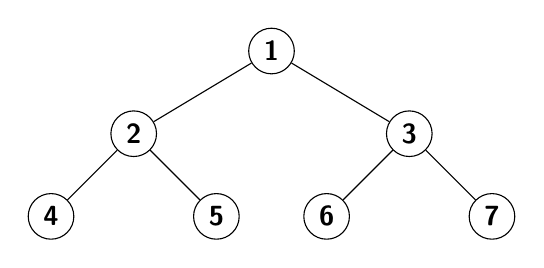
\begin{tikzpicture} [scale = 0.7,level 1/.style = {sibling distance = 5cm, level distance = 1.5cm},
						  level 2/.style = {sibling distance = 3cm}]
	\node [arn_n] {1}
	 child{ node [arn_n] {2} 
	            child{node [arn_n] {4}} 
	            child{node [arn_n] {5}}	
	      }
	 child{node [arn_n] {3} 
	            child{node [arn_n] {6}} 
	            child{node [arn_n] {7}}	
	      };
	\end{tikzpicture}

\end{center} 

The same principles apply in the case of Finger Trees, which is based on a full 2-3 tree, with labels in the leafs only.


\chapter{Implementation}

\section{FingerTrees - Introduction} 
	Finger Trees are a data structure introduced by Ralph Hinze and Robert Patinsson, based on Okasaki's principle of implicit recursive slowdown. \\ 
Initially meant as a double ended queue with constant amortized time append, their structure, together with the cached measurements, allow specialization to Random Access Sequences, or Priority Queues by simple instantiation. \\ 
 
 	The underlying structure is that of a full 2-3 tree, with labels solely at the leafs. For efficient insertion and deletions, the tree is surrounded by buffers at each level, which amortize the cost of appending at either end. Furthermore, the data structure is accompanied by a measurement function and a binary operator, such that the reduced measures of all nodes in a subtree is cached in all the joints. These are necessary for searching or splitting.
 		
\begin{figure} 
	\centering
	\begin{tikzpicture} [scale = 0.7,level 1/.style = {sibling distance = 2cm, level distance = 1.5cm},					  
		level 2/.style = {sibling distance = 4cm, level distance = 1.5cm},
		level 3/.style = {sibling distance = 2cm, level distance = 1.5cm}]
		\node [deep] {}
		 child{node [digit] {∙ ∙ ∙} 	
		      }
		 child{node [deep] {}
		 		child{node [node] {}
		 				child{node [digit] {∙ ∙ ∙ ∙}}
		 				child{node [digit] {∙}}
		 			}
			 	child{node [deep] {}
			 			child{node [leaf] {}}
			 		}
		 		child{node [node] {}
		 				child{node [digit] {∙ ∙}}
		 				child{node [digit] {∙}} 
		 				child{node [digit] {∙ ∙ ∙}}
		 			}
		 	 } 
		 child{node [digit] {∙ ∙}	
		      };
	\end{tikzpicture}
	\caption{Example finger tree}
	\label{fig:ftex1}
\end{figure} 

\subsection{Invariants}

The efficiency is achieved by keeping two invariants on the data structure:
\begin{itemize}
	\item The tree is full and all the leaves occur on the last level. 
	\item The measurements are correct\footnote{•}
\end{itemize}

Working in Agda, a dependently typed language, which moreover allows the use of nested types, we can keep these invariants soley in the type of the Finger Tree. More specifically,
\begin{itemize}
	\item The nested typing will ensure fullness of the tree.
	\item Choosing measurements as the type index ensures their correctness.  
\end{itemize} 

\subsection{Previous Work}

Finger Trees have been previously implemented and proved correct. I will outline some previous results, as well as their limitations, providing more incentives for this dissertation. I have included all related implementations I could find and I do not guarantee they are the only ones.

\begin{itemize}
\item Basic Implementation in Agda. \\
This version can be found on GitHub\footnote{•}. Its mentioned intention is to closely follow the original paper. It also uses introduces the idea of Sizing, although only in the type declaration (and constructors). Since the constraints are not present in functions that modify the data type, they do not really aid correctness proofs. It has no proofs associated with it, and it didn't type check on my machine.
\item Implementation in Coq. \\
This implementation is provided by Matthiew Souzeau\cite{coq} as a proof of concept for Russell, a Coq extension. I have drawn great inspiration from that paper, and I was particularly drawn by its small caveat, onto which I will return at the end of this chapter. Although a full and working implementation, I argue that this dissertation is valuable in its own, given my aforementioned reasons for choosing Agda as the programming language, and providing a solution to some caveats.
\item Implementation in Isabelle. \\
Another working implementation has been done in Isabelle. However, this implementation diverges from the original specification of the data structure, removing the nesting. The two invariants that I have mentioned are maintained explicitly, due to the lack of dependent types.\\ 
The implementation of this data structure in both Coq and Isabelle, two established theorem provers might argue both for the complexity involved, and for its interesting particularities.
\end{itemize}

\section{Finger Trees - Implementation}

\subsection{Data type declaration}

The Finger Tree is originally polymorphic in two types:
\begin{itemize}
\item \textbf{A} : this is the type of the elements that are contained in the Finger Tree 
\item \textbf{V} : this is the type of measures. 
\end{itemize} 


In order to to mimic Haskell's typeclasses, I have carried around, for each A and V, two constructs:

\begin{itemize} 
\item \textbf{Monoid\footnote{see AlgebraStructures.agda} V}: which contains a neutral element(\textbf{ε}), a binary operator(\textbf{∙}), and the monoid axioms, and a comparison operator.
\item \textbf{Measured A V} : which consists of a norm function  :  \textbf{$\Vert\_\Vert : \nolinebreak A \rightarrow V$}
\end{itemize} 


\textbf{Node} corresponds to nodes in the underlying 2-3 tree implementation, having two constructors that contain two and respectively three items. Moreover, \textbf{Node}s can only be constructed if provided with a measurement tag and a correctness proof.
  
\begin{code}
\\
\>\AgdaKeyword{data} \AgdaDatatype{Node} \AgdaSymbol{\{}\AgdaBound{a}\AgdaSymbol{\}} \AgdaSymbol{(}\AgdaBound{A} \AgdaSymbol{:} \AgdaPrimitiveType{Set} \AgdaBound{a}\AgdaSymbol{)(}\AgdaBound{V} \AgdaSymbol{:} \AgdaPrimitiveType{Set} \AgdaBound{a} \AgdaSymbol{)}\<%
\\
\>[0]\AgdaIndent{10}{}\<[10]%
\>[10]\AgdaSymbol{⦃} \AgdaBound{mo} \AgdaSymbol{:} \AgdaRecord{Monoid} \AgdaBound{V} \AgdaSymbol{⦄}\<%
\\
\>[0]\AgdaIndent{10}{}\<[10]%
\>[10]\AgdaSymbol{⦃} \AgdaBound{m} \AgdaSymbol{:} \AgdaRecord{Measured} \AgdaBound{A} \AgdaBound{V} \AgdaSymbol{⦄} \AgdaSymbol{:} \AgdaPrimitiveType{Set} \AgdaBound{a} \AgdaKeyword{where}\<%
\\
\>[0]\AgdaIndent{2}{}\<[2]%
\>[2]\AgdaInductiveConstructor{Node2} \AgdaSymbol{:} \AgdaSymbol{(}\AgdaBound{v} \AgdaSymbol{:} \AgdaBound{V}\AgdaSymbol{)}\<%
\\
\>[2]\AgdaIndent{8}{}\<[8]%
\>[8]\AgdaSymbol{→} \AgdaSymbol{(}\AgdaBound{x} \AgdaSymbol{:} \AgdaBound{A}\AgdaSymbol{)} \AgdaSymbol{→} \AgdaSymbol{(}\AgdaBound{y} \AgdaSymbol{:} \AgdaBound{A}\AgdaSymbol{)}\<%
\\
\>[2]\AgdaIndent{8}{}\<[8]%
\>[8]\AgdaSymbol{→} \<[11]%
\>[11]\AgdaSymbol{(}\AgdaBound{v} \AgdaDatatype{≡} \AgdaField{∥} \AgdaBound{x} \AgdaField{∥} \AgdaField{∙} \AgdaField{∥} \AgdaBound{y} \AgdaField{∥}\AgdaSymbol{)}\<%
\\
\>[2]\AgdaIndent{8}{}\<[8]%
\>[8]\AgdaSymbol{→} \AgdaDatatype{Node} \AgdaBound{A} \AgdaBound{V}\<%
\\
\>[0]\AgdaIndent{2}{}\<[2]%
\>[2]\AgdaInductiveConstructor{Node3} \AgdaSymbol{:} \AgdaSymbol{(}\AgdaBound{v} \AgdaSymbol{:} \AgdaBound{V}\AgdaSymbol{)}\<%
\\
\>[2]\AgdaIndent{8}{}\<[8]%
\>[8]\AgdaSymbol{→} \AgdaSymbol{(}\AgdaBound{x} \AgdaSymbol{:} \AgdaBound{A}\AgdaSymbol{)} \AgdaSymbol{→} \AgdaSymbol{(}\AgdaBound{y} \AgdaSymbol{:} \AgdaBound{A}\AgdaSymbol{)} \AgdaSymbol{→} \AgdaSymbol{(}\AgdaBound{z} \AgdaSymbol{:} \AgdaBound{A}\AgdaSymbol{)}\<%
\\
\>[2]\AgdaIndent{8}{}\<[8]%
\>[8]\AgdaSymbol{→} \AgdaSymbol{(}\AgdaBound{v} \AgdaDatatype{≡} \AgdaField{∥} \AgdaBound{x} \AgdaField{∥} \AgdaField{∙} \AgdaField{∥} \AgdaBound{y} \AgdaField{∥} \AgdaField{∙} \AgdaField{∥} \AgdaBound{z} \AgdaField{∥}\AgdaSymbol{)}\<%
\\
\>[2]\AgdaIndent{8}{}\<[8]%
\>[8]\AgdaSymbol{→} \AgdaDatatype{Node} \AgdaBound{A} \AgdaBound{V}\<%
\\
\end{code}
\textbf{Digit}s were in presented in the original paper as lists, but this definition limits them to have one to four elements.

\begin{code}
\\
\>\AgdaKeyword{data} \AgdaDatatype{Digit} \AgdaSymbol{\{}\AgdaBound{a}\AgdaSymbol{\}} \AgdaSymbol{(}\AgdaBound{A} \AgdaSymbol{:} \AgdaPrimitiveType{Set} \AgdaBound{a}\AgdaSymbol{):} \AgdaPrimitiveType{Set} \AgdaBound{a} \AgdaKeyword{where}\<%
\\
\>[0]\AgdaIndent{2}{}\<[2]%
\>[2]\AgdaInductiveConstructor{One} \<[8]%
\>[8]\AgdaSymbol{:} \AgdaBound{A} \AgdaSymbol{→} \AgdaDatatype{Digit} \AgdaBound{A}\<%
\\
\>[0]\AgdaIndent{2}{}\<[2]%
\>[2]\AgdaInductiveConstructor{Two} \<[8]%
\>[8]\AgdaSymbol{:} \AgdaBound{A} \AgdaSymbol{→} \AgdaBound{A} \AgdaSymbol{→} \AgdaDatatype{Digit} \AgdaBound{A}\<%
\\
\>[0]\AgdaIndent{2}{}\<[2]%
\>[2]\AgdaInductiveConstructor{Three} \AgdaSymbol{:} \AgdaBound{A} \AgdaSymbol{→} \AgdaBound{A} \AgdaSymbol{→} \AgdaBound{A} \AgdaSymbol{→} \AgdaDatatype{Digit} \AgdaBound{A}\<%
\\
\>[0]\AgdaIndent{2}{}\<[2]%
\>[2]\AgdaInductiveConstructor{Four} \<[8]%
\>[8]\AgdaSymbol{:} \AgdaBound{A} \AgdaSymbol{→} \AgdaBound{A} \AgdaSymbol{→} \AgdaBound{A} \AgdaSymbol{→} \AgdaBound{A} \AgdaSymbol{→} \AgdaDatatype{Digit} \AgdaBound{A}\<%
\\
\end{code}
Finally, the \textbf{FingerTree} is a family of types, indexed by a measurement $\mu$. The measurement's correctness is enforced in all the constructors. Note the nested type and the universal quantification over possible sizes for the recursive call. Apart from the measurement addition, the rest corresponds to the original paper.


\begin{code}
\\
\>\AgdaKeyword{data} \AgdaDatatype{FingerTree} \AgdaSymbol{\{}\AgdaBound{a}\AgdaSymbol{\}} \AgdaSymbol{(}\AgdaBound{A} \AgdaSymbol{:} \AgdaPrimitiveType{Set} \AgdaBound{a}\AgdaSymbol{)(}\AgdaBound{V} \AgdaSymbol{:} \AgdaPrimitiveType{Set} \AgdaBound{a}\AgdaSymbol{)}\<%
\\
\>[2]\AgdaIndent{16}{}\<[16]%
\>[16]\AgdaSymbol{⦃} \AgdaBound{mo} \AgdaSymbol{:} \AgdaRecord{Monoid} \AgdaBound{V} \AgdaSymbol{⦄}\<%
\\
\>[2]\AgdaIndent{16}{}\<[16]%
\>[16]\AgdaSymbol{⦃} \AgdaBound{m} \AgdaSymbol{:} \AgdaRecord{Measured} \AgdaBound{A} \AgdaBound{V} \AgdaSymbol{⦄} \AgdaSymbol{:}\<%
\\
\>[2]\AgdaIndent{16}{}\<[16]%
\>[16]\AgdaSymbol{\{}\AgdaBound{μ} \AgdaSymbol{:} \AgdaBound{V}\AgdaSymbol{\}} \AgdaSymbol{→} \AgdaPrimitiveType{Set} \AgdaBound{a} \AgdaKeyword{where}\<%
\\
\>[0]\AgdaIndent{2}{}\<[2]%
\>[2]\AgdaInductiveConstructor{Empty} \<[9]%
\>[9]\AgdaSymbol{:} \<[12]%
\>[12]\AgdaDatatype{FingerTree} \AgdaBound{A} \AgdaBound{V} \AgdaSymbol{\{}\AgdaField{ε}\AgdaSymbol{\}}\<%
\\
\>[0]\AgdaIndent{2}{}\<[2]%
\>[2]\AgdaInductiveConstructor{Single} \AgdaSymbol{:} \<[12]%
\>[12]\AgdaSymbol{(}\AgdaBound{e} \AgdaSymbol{:} \AgdaBound{A}\AgdaSymbol{)} \AgdaSymbol{→} \AgdaDatatype{FingerTree} \AgdaBound{A} \AgdaBound{V} \AgdaSymbol{\{}\AgdaField{∥} \AgdaBound{e} \AgdaField{∥}\AgdaSymbol{\}}\<%
\\
\>[0]\AgdaIndent{2}{}\<[2]%
\>[2]\AgdaInductiveConstructor{Deep} \<[9]%
\>[9]\AgdaSymbol{:} \<[12]%
\>[12]\AgdaSymbol{\{}\AgdaBound{s} \AgdaSymbol{:} \AgdaBound{V}\AgdaSymbol{\}}\<%
\\
\>[2]\AgdaIndent{10}{}\<[10]%
\>[10]\AgdaSymbol{→} \AgdaSymbol{(}\AgdaBound{pr} \AgdaSymbol{:} \AgdaDatatype{Digit} \AgdaBound{A}\AgdaSymbol{)}\<%
\\
\>[2]\AgdaIndent{10}{}\<[10]%
\>[10]\AgdaSymbol{→} \AgdaDatatype{FingerTree} \AgdaSymbol{(}\AgdaDatatype{Node} \AgdaBound{A} \AgdaBound{V}\AgdaSymbol{)} \AgdaBound{V} \AgdaSymbol{\{}\AgdaBound{s}\AgdaSymbol{\}}\<%
\\
\>[2]\AgdaIndent{10}{}\<[10]%
\>[10]\AgdaSymbol{→} \AgdaSymbol{(}\AgdaBound{sf} \AgdaSymbol{:} \AgdaDatatype{Digit} \AgdaBound{A}\AgdaSymbol{)}\<%
\\
\>[2]\AgdaIndent{10}{}\<[10]%
\>[10]\AgdaSymbol{→} \AgdaDatatype{FingerTree} \AgdaBound{A} \AgdaBound{V} \AgdaSymbol{\{}\AgdaFunction{measure-digit} \AgdaBound{pr} \AgdaField{∙} \AgdaBound{s} \AgdaField{∙} \AgdaFunction{measure-digit} \AgdaBound{sf}\AgdaSymbol{\}}\<%
\\
\end{code}

\subparagraph{Smart Constructors}
We also build smart constructors that fill in the measurement, provided with the appropriate number of elements

\begin{code}
\\
\>\AgdaFunction{node2} \AgdaSymbol{:} \AgdaSymbol{∀} \AgdaSymbol{\{}\AgdaBound{a}\AgdaSymbol{\}} \AgdaSymbol{\{}\AgdaBound{A} \AgdaSymbol{:} \AgdaPrimitiveType{Set} \AgdaBound{a}\AgdaSymbol{\}\{}\AgdaBound{V} \AgdaSymbol{:} \AgdaPrimitiveType{Set} \AgdaBound{a} \AgdaSymbol{\}}\<%
\\
\>[0]\AgdaIndent{8}{}\<[8]%
\>[8]\AgdaSymbol{⦃} \AgdaBound{mo} \AgdaSymbol{:} \AgdaRecord{Monoid} \AgdaBound{V} \AgdaSymbol{⦄}\<%
\\
\>[0]\AgdaIndent{8}{}\<[8]%
\>[8]\AgdaSymbol{⦃} \AgdaBound{m} \AgdaSymbol{:} \AgdaRecord{Measured} \AgdaBound{A} \AgdaBound{V} \AgdaSymbol{⦄}\<%
\\
\>[0]\AgdaIndent{8}{}\<[8]%
\>[8]\AgdaSymbol{→} \AgdaBound{A} \AgdaSymbol{→} \AgdaBound{A} \AgdaSymbol{→} \AgdaDatatype{Node} \AgdaBound{A} \AgdaBound{V}\<%
\\
\>\AgdaFunction{node2} \AgdaBound{x} \AgdaBound{y} \AgdaSymbol{=} \AgdaInductiveConstructor{Node2} \AgdaSymbol{(}\AgdaField{∥} \AgdaBound{x} \AgdaField{∥} \AgdaField{∙} \AgdaField{∥} \AgdaBound{y} \AgdaField{∥}\AgdaSymbol{)} \AgdaBound{x} \AgdaBound{y} \AgdaInductiveConstructor{refl}\<%
\\
%
\\
\>\AgdaFunction{node3} \AgdaSymbol{:} \AgdaSymbol{∀} \AgdaSymbol{\{}\AgdaBound{a}\AgdaSymbol{\}} \AgdaSymbol{\{}\AgdaBound{A} \AgdaSymbol{:} \AgdaPrimitiveType{Set} \AgdaBound{a}\AgdaSymbol{\}\{}\AgdaBound{V} \AgdaSymbol{:} \AgdaPrimitiveType{Set} \AgdaBound{a} \AgdaSymbol{\}}\<%
\\
\>[0]\AgdaIndent{8}{}\<[8]%
\>[8]\AgdaSymbol{⦃} \AgdaBound{mo} \AgdaSymbol{:} \AgdaRecord{Monoid} \AgdaBound{V} \AgdaSymbol{⦄}\<%
\\
\>[0]\AgdaIndent{8}{}\<[8]%
\>[8]\AgdaSymbol{⦃} \AgdaBound{m} \AgdaSymbol{:} \AgdaRecord{Measured} \AgdaBound{A} \AgdaBound{V} \AgdaSymbol{⦄}\<%
\\
\>[0]\AgdaIndent{8}{}\<[8]%
\>[8]\AgdaSymbol{→} \AgdaBound{A} \AgdaSymbol{→} \AgdaBound{A} \AgdaSymbol{→} \AgdaBound{A} \AgdaSymbol{→} \AgdaDatatype{Node} \AgdaBound{A} \AgdaBound{V}\<%
\\
\>\AgdaFunction{node3} \AgdaBound{x} \AgdaBound{y} \AgdaBound{z} \AgdaSymbol{=} \AgdaInductiveConstructor{Node3} \AgdaSymbol{(}\AgdaField{∥} \AgdaBound{x} \AgdaField{∥} \AgdaField{∙} \AgdaField{∥} \AgdaBound{y} \AgdaField{∥} \AgdaField{∙} \AgdaField{∥} \AgdaBound{z} \AgdaField{∥}\AgdaSymbol{)} \AgdaBound{x} \AgdaBound{y} \AgdaBound{z} \AgdaInductiveConstructor{refl}\<%
\\
\end{code}
\subsection{Graphical example}

Considering Figure, \ref{fig:ftex1}, I have colour-coded the nodes as follows:
\begin{table}[h!]
\centering
\begin{tabular}{c c}
Symbol & Constructor \\ 
\hline

\begin{tikzpicture} [scale = 0.7,level 1/.style = {sibling distance = 2cm, level distance = 1.5cm}]		  
		\node [deep] {};
\end{tikzpicture} & Deep \\
 

\begin{tikzpicture} [scale = 0.7,level 1/.style = {sibling distance = 2cm, level distance = 1.5cm}]		  
		\node [node] {};
\end{tikzpicture} & Node \\
\begin{tikzpicture} [scale = 0.7,level 1/.style = {sibling distance = 2cm, level distance = 1.5cm}]		  
		\node [digit] {∙ ∙ ∙};
\end{tikzpicture} & Digit (of various lengths) \\


\begin{tikzpicture} [scale = 0.7,level 1/.style = {sibling distance = 2cm, level distance = 1.5cm}]		  
		\node [leaf] {};
\end{tikzpicture} & A \\
\hline
\end{tabular}
\end{table}


\subsection{Indexing on the measurement}

The reason for indexing on the measurement is twofold. Firstly, we index on the measurement in order to verify the correctness of the measurement in operations such as appending an element or splitting. Secondly, the index was chosen in order to allow implementing a 'size' that depends on all elements in the finger tree. 

Consider a sizing that would take into account the shape of the tree only (as it is the case of Size described previously). 

\begin{figure}[h!]
\centering 
	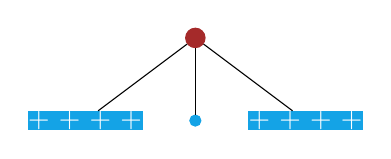
\begin{tikzpicture} [scale = 0.7,level 1/.style = {sibling distance = 2cm, level distance = 1.5cm},					  
		level 2/.style = {sibling distance = 4cm, level distance = 1.5cm},
		level 3/.style = {sibling distance = 2cm, level distance = 1.5cm}]
		\node [deep] {}
		 child{node [digit] {+ + + +} 	
		      }
		 child{node [leaf] {}}
		 child{node [digit] {+ + + +}	
		      };
	\end{tikzpicture}
	\caption{Bigger Finger Tree}
	\label{fig:ftex2}
	\vspace{3mm}
	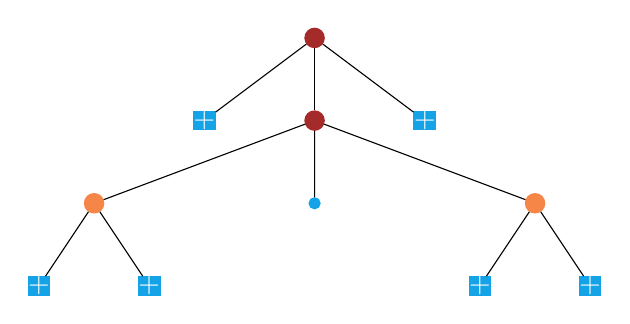
\begin{tikzpicture} [scale = 0.7,level 1/.style = {sibling distance = 2cm, level distance = 1.5cm},					  
		level 2/.style = {sibling distance = 4cm, level distance = 1.5cm},
		level 3/.style = {sibling distance = 2cm, level distance = 1.5cm}]
		\node [deep] {}
		 child{node [digit] {+} 	
		      }
		 child{node [deep] {}
		 		child{node [node] {}
		 				child{node [digit] {+}}
		 				child{node [digit] {+}}
		 			}
			 	child{node [leaf] {}}
		 		child{node [node] {}
		 				child{node [digit] {+}} 
		 				child{node [digit] {+}}
		 			}
		 	 } 
		 child{node [digit] {+}	
		      };
	\end{tikzpicture}
	\caption{Smaller finger Tree}
	\label{fig:ftex3}
\end{figure} 

In Figures \ref{fig:ftex2} and \ref{fig:ftex3}, it is an ambiguous question which of the two trees should be considered to have a bigger size. \textit{Size} implements a partial order between data types, with no definite reference points, whereas here we are concerned with an absolute order. \\
As suggested by Matthew Souzeau \cite{coq_finger_tree}, a sizing that reflects the number of elements is ideal. We can use the already existing measurement index to achive this goal.

\subsection{\textit{Cons} and \textit{Snoc}}

\textit{Cons} is the operator that appends an element to the left of the finger tree. 

The implementation is straight forward if there is room in the left-most digit. Otherwise, we have to recursively insert and reform parts of the finger tree.

Ultimately, for the correctness part, we are concerned whether the output tree is a correct finger tree (enforced by the type) with a correct measurement. 
\begin{align*}
\intertext{That is, by inserting an element x,}
	\Vert x \triangleleft ft \Vert = \Vert x \Vert \cdot \Vert ft \Vert
\end{align*}
\begin{figure}[h!]
\centering 
\subfloat[Before Cons]
{
	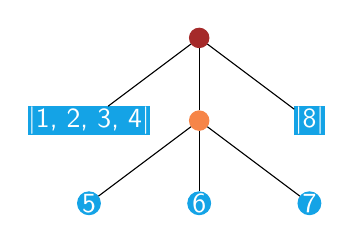
\begin{tikzpicture} [scale = 0.7,level 1/.style = {sibling distance = 2cm, level distance = 1.5cm},					  
		level 2/.style = {sibling distance = 2cm, level distance = 1.5cm},
		level 3/.style = {sibling distance = 2cm, level distance = 1.5cm}]
		\node [deep] {}
		 child{node [digit] {$|$1, 2, 3, 4$|$} 	
		      }
		 child{node [node] {}
				child {node [leaf] {5}}
				child {node [leaf] {6}}
				child {node [leaf] {7}}
		}
		 child{node [digit] {$|$8$|$}	
		      };
	\end{tikzpicture}
}
\qquad
\subfloat[After Cons]
{
	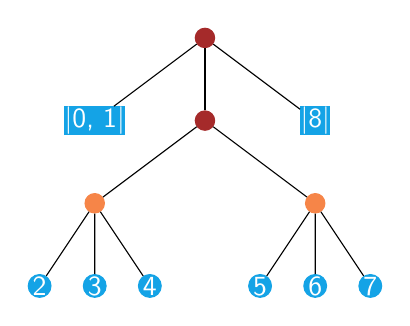
\begin{tikzpicture} [scale = 0.7,level 1/.style = {sibling distance = 2cm, level distance = 1.5cm},					  
		level 2/.style = {sibling distance = 4cm, level distance = 1.5cm},
		level 3/.style = {sibling distance = 1cm, level distance = 1.5cm}]
		\node [deep] {}
		 child{node [digit] {$|$0, 1$|$} 	
		      }
		 child{node [deep] {}
		 		child{node [node] {}
		 				child{node [leaf] {2}}
		 				child{node [leaf] {3}}
		 				child{node [leaf] {4}}
		 			}
			 	child{node [node] {}
		 				child{node [leaf] {5}} 
		 				child{node [leaf] {6}}
		 				child{node [leaf] {7}}
		 			}
		 	 } 
		 child{node [digit] {$|$8$|$}	
		      };
	\end{tikzpicture}
}
	\caption{Recursive cons operation}
	\label{fig:ftex3}
\end{figure}



\begin{code}
\\
\\
\\
\\
\\
\>\AgdaFunction{\_◁\_} \AgdaSymbol{:} \AgdaSymbol{∀} \AgdaSymbol{\{}\AgdaBound{a}\AgdaSymbol{\}} \AgdaSymbol{\{}\AgdaBound{A} \AgdaSymbol{:} \AgdaPrimitiveType{Set} \AgdaBound{a}\AgdaSymbol{\}} \AgdaSymbol{\{}\AgdaBound{V} \AgdaSymbol{:} \AgdaPrimitiveType{Set} \AgdaBound{a}\AgdaSymbol{\}}\<%
\\
\>[2]\AgdaIndent{6}{}\<[6]%
\>[6]\AgdaSymbol{⦃} \AgdaBound{mo} \AgdaSymbol{:} \AgdaRecord{Monoid} \AgdaBound{V} \AgdaSymbol{⦄}\<%
\\
\>[2]\AgdaIndent{6}{}\<[6]%
\>[6]\AgdaSymbol{⦃} \AgdaBound{m} \AgdaSymbol{:} \AgdaRecord{Measured} \AgdaBound{A} \AgdaBound{V} \AgdaSymbol{⦄}\<%
\\
\>[2]\AgdaIndent{6}{}\<[6]%
\>[6]\AgdaSymbol{\{}\AgdaBound{s} \AgdaSymbol{:} \AgdaBound{V}\AgdaSymbol{\}}\<%
\\
\>[2]\AgdaIndent{6}{}\<[6]%
\>[6]\AgdaSymbol{→} \AgdaSymbol{(}\AgdaBound{x} \AgdaSymbol{:} \AgdaBound{A}\AgdaSymbol{)}\<%
\\
\>[2]\AgdaIndent{6}{}\<[6]%
\>[6]\AgdaSymbol{→} \AgdaDatatype{FingerTree} \AgdaBound{A} \AgdaBound{V} \AgdaSymbol{⦃} \AgdaBound{mo} \AgdaSymbol{⦄} \AgdaSymbol{⦃} \AgdaBound{m} \AgdaSymbol{⦄} \AgdaSymbol{\{}\AgdaBound{s}\AgdaSymbol{\}}\<%
\\
\>[2]\AgdaIndent{6}{}\<[6]%
\>[6]\AgdaSymbol{→} \AgdaDatatype{FingerTree} \AgdaBound{A} \AgdaBound{V} \AgdaSymbol{⦃} \AgdaBound{mo} \AgdaSymbol{⦄} \AgdaSymbol{⦃} \AgdaBound{m} \AgdaSymbol{⦄} \AgdaSymbol{\{}\AgdaField{∥} \AgdaBound{x} \AgdaField{∥} \AgdaField{∙} \AgdaBound{s}\AgdaSymbol{\}}\<%
\\
\end{code}
Each case in the definition is accompanied by a proof that the measurement of the output finger tree is correct with respect to the topmost definition. These proofs are all derived from monoid properties imposed on the operation.


\begin{code} 
\>\AgdaFunction{\_◁\_} \AgdaSymbol{\{}\AgdaBound{l}\AgdaSymbol{\}} \AgdaSymbol{\{}\AgdaBound{A}\AgdaSymbol{\}} \AgdaSymbol{\{}\AgdaBound{V}\AgdaSymbol{\}} \AgdaSymbol{⦃} \AgdaBound{mo} \AgdaSymbol{⦄} \AgdaBound{a} \AgdaInductiveConstructor{Empty}\<%
\\
\>[0]\AgdaIndent{2}{}\<[2]%
\>[2]\AgdaKeyword{rewrite} \AgdaSymbol{(}\AgdaField{Monoid.ε-right} \AgdaBound{mo}\AgdaSymbol{)} \AgdaField{∥} \AgdaBound{a} \AgdaField{∥}\<%
\\
\>[0]\AgdaIndent{2}{}\<[2]%
\>[2]\AgdaSymbol{=} \AgdaInductiveConstructor{Single} \AgdaSymbol{\{}\AgdaBound{l}\AgdaSymbol{\}\{}\AgdaBound{A}\AgdaSymbol{\}\{}\AgdaBound{V}\AgdaSymbol{\}} \AgdaBound{a}\<%
\\
\>\AgdaFunction{\_◁\_} \AgdaSymbol{\{}\AgdaBound{l}\AgdaSymbol{\}} \AgdaSymbol{\{}\AgdaBound{A}\AgdaSymbol{\}} \AgdaSymbol{\{}\AgdaBound{V}\AgdaSymbol{\}} \AgdaSymbol{⦃} \AgdaBound{mo} \AgdaSymbol{⦄} \AgdaSymbol{⦃} \AgdaBound{m} \AgdaSymbol{⦄} \AgdaSymbol{\{}\AgdaSymbol{.(}\AgdaField{∥} \AgdaBound{e} \AgdaField{∥}\AgdaSymbol{)}\AgdaSymbol{\}} \AgdaBound{a} \AgdaSymbol{(}\AgdaInductiveConstructor{Single} \AgdaBound{e}\AgdaSymbol{)}\<%
\\
\>[0]\AgdaIndent{2}{}\<[2]%
\>[2]\AgdaKeyword{rewrite} \AgdaFunction{assoc-lemma1} \AgdaSymbol{⦃} \AgdaBound{mo} \AgdaSymbol{⦄} \AgdaSymbol{⦃} \AgdaBound{m} \AgdaSymbol{⦄} \AgdaBound{a} \AgdaBound{e}\<%
\\
\>[0]\AgdaIndent{2}{}\<[2]%
\>[2]\AgdaSymbol{=} \AgdaInductiveConstructor{Deep} \AgdaSymbol{(}\AgdaInductiveConstructor{One} \AgdaBound{a}\AgdaSymbol{)} \AgdaInductiveConstructor{Empty} \AgdaSymbol{(}\AgdaInductiveConstructor{One} \AgdaBound{e}\AgdaSymbol{)}\<%
\\
\>\AgdaBound{a} \AgdaFunction{◁} \AgdaInductiveConstructor{Deep} \AgdaSymbol{(}\AgdaInductiveConstructor{One} \AgdaBound{b}\AgdaSymbol{)} \AgdaBound{ft} \AgdaBound{sf}\<%
\\
\>[0]\AgdaIndent{2}{}\<[2]%
\>[2]\AgdaKeyword{rewrite} \AgdaField{∙-assoc} \AgdaSymbol{(}\AgdaField{∥} \AgdaBound{a} \AgdaField{∥}\AgdaSymbol{)} \AgdaSymbol{(}\AgdaField{∥} \AgdaBound{b} \AgdaField{∥}\AgdaSymbol{)} \AgdaSymbol{(}\AgdaFunction{measure-tree} \AgdaBound{ft} \AgdaField{∙} \AgdaFunction{measure-digit} \AgdaBound{sf}\AgdaSymbol{)}\<%
\\
\>[0]\AgdaIndent{2}{}\<[2]%
\>[2]\AgdaSymbol{=} \AgdaInductiveConstructor{Deep} \AgdaSymbol{(}\AgdaInductiveConstructor{Two} \AgdaBound{a} \AgdaBound{b}\AgdaSymbol{)} \AgdaBound{ft} \AgdaBound{sf}\<%
\\
\>\AgdaBound{a} \AgdaFunction{◁} \AgdaInductiveConstructor{Deep} \AgdaSymbol{(}\AgdaInductiveConstructor{Two} \AgdaBound{b} \AgdaBound{c}\AgdaSymbol{)} \AgdaBound{ft} \AgdaBound{sf}\<%
\\
\>[0]\AgdaIndent{2}{}\<[2]%
\>[2]\AgdaKeyword{rewrite} \AgdaField{∙-assoc} \AgdaSymbol{(}\AgdaField{∥} \AgdaBound{a} \AgdaField{∥}\AgdaSymbol{)} \AgdaSymbol{(}\AgdaField{∥} \AgdaBound{b} \AgdaField{∥} \AgdaField{∙} \AgdaField{∥} \AgdaBound{c} \AgdaField{∥}\AgdaSymbol{)} \AgdaSymbol{(}\AgdaFunction{measure-tree} \AgdaBound{ft} \AgdaField{∙} \AgdaFunction{measure-digit} \AgdaBound{sf}\AgdaSymbol{)}\<%
\\
\>[0]\AgdaIndent{2}{}\<[2]%
\>[2]\AgdaSymbol{=} \AgdaInductiveConstructor{Deep} \AgdaSymbol{(}\AgdaInductiveConstructor{Three} \AgdaBound{a} \AgdaBound{b} \AgdaBound{c}\AgdaSymbol{)} \AgdaBound{ft} \AgdaBound{sf}\<%
\\
\>\AgdaBound{a} \AgdaFunction{◁} \AgdaInductiveConstructor{Deep} \AgdaSymbol{(}\AgdaInductiveConstructor{Three} \AgdaBound{b} \AgdaBound{c} \AgdaBound{d}\AgdaSymbol{)} \AgdaBound{ft} \AgdaBound{sf}\<%
\\
\>[0]\AgdaIndent{2}{}\<[2]%
\>[2]\AgdaKeyword{rewrite} \AgdaField{∙-assoc} \AgdaSymbol{(}\AgdaField{∥} \AgdaBound{a} \AgdaField{∥}\AgdaSymbol{)} \AgdaSymbol{(}\AgdaField{∥} \AgdaBound{b} \AgdaField{∥} \AgdaField{∙} \AgdaField{∥} \AgdaBound{c} \AgdaField{∥} \AgdaField{∙} \AgdaField{∥} \AgdaBound{d} \AgdaField{∥}\AgdaSymbol{)} \AgdaSymbol{(}\AgdaFunction{measure-tree} \AgdaBound{ft} \AgdaField{∙} \AgdaFunction{measure-digit} \AgdaBound{sf}\AgdaSymbol{)}\<%
\\
\>[0]\AgdaIndent{2}{}\<[2]%
\>[2]\AgdaSymbol{=} \AgdaInductiveConstructor{Deep} \AgdaSymbol{(}\AgdaInductiveConstructor{Four} \AgdaBound{a} \AgdaBound{b} \AgdaBound{c} \AgdaBound{d}\AgdaSymbol{)} \AgdaBound{ft} \AgdaBound{sf}\<%
\\
\>\AgdaBound{a} \AgdaFunction{◁} \AgdaInductiveConstructor{Deep} \AgdaSymbol{(}\AgdaInductiveConstructor{Four} \AgdaBound{b} \AgdaBound{c} \AgdaBound{d} \AgdaBound{e}\AgdaSymbol{)} \AgdaBound{ft} \AgdaBound{sf}\<%
\\
\>[0]\AgdaIndent{2}{}\<[2]%
\>[2]\AgdaKeyword{rewrite} \AgdaFunction{assoc-lemma2} \AgdaBound{a} \AgdaBound{b} \AgdaBound{c} \AgdaBound{d} \AgdaBound{e} \AgdaSymbol{(}\AgdaFunction{measure-tree} \AgdaBound{ft}\AgdaSymbol{)} \AgdaSymbol{(}\AgdaFunction{measure-digit} \AgdaBound{sf}\AgdaSymbol{)}\<%
\\
\>[0]\AgdaIndent{2}{}\<[2]%
\>[2]\AgdaSymbol{=} \AgdaInductiveConstructor{Deep} \AgdaSymbol{(}\AgdaInductiveConstructor{Two} \AgdaBound{a} \AgdaBound{b}\AgdaSymbol{)} \AgdaSymbol{((}\AgdaFunction{node3} \AgdaBound{c} \AgdaBound{d} \AgdaBound{e}\AgdaSymbol{)} \AgdaFunction{◁} \AgdaBound{ft}\AgdaSymbol{)} \AgdaBound{sf}\<%
\\
\end{code}

The Finger Tree operations are symmetric on the middle, so the construction of the snoc operator is exactly dual. It's implementation is provided in the source code.

\subsection{\textit{toList}}

We will need to prove properties of the finger trees with respect to the elements they contain and their relative position. Therefore, it is handy to be able to transform them to lists, as they encode these properties simply.


This is the conversion between a finger tree and a list\footnote{
toList-dig is a straightforward conversion.}\footnote{flatten-list transforms a list of Nodes into a list of As.}

\begin{code}
\\
\>\AgdaFunction{toList-ft} \AgdaSymbol{:} \AgdaSymbol{∀} \AgdaSymbol{\{}\AgdaBound{a}\AgdaSymbol{\}\{}\AgdaBound{A} \AgdaSymbol{:} \AgdaPrimitiveType{Set} \AgdaBound{a}\AgdaSymbol{\}\{}\AgdaBound{V} \AgdaSymbol{:} \AgdaPrimitiveType{Set} \AgdaBound{a} \AgdaSymbol{\}}\<%
\\
\>[0]\AgdaIndent{10}{}\<[10]%
\>[10]\AgdaSymbol{⦃} \AgdaBound{mo} \AgdaSymbol{:} \AgdaRecord{Monoid} \AgdaBound{V} \AgdaSymbol{⦄}\<%
\\
\>[0]\AgdaIndent{10}{}\<[10]%
\>[10]\AgdaSymbol{⦃} \AgdaBound{m} \AgdaSymbol{:} \AgdaRecord{Measured} \AgdaBound{A} \AgdaBound{V} \AgdaSymbol{⦄} \AgdaSymbol{\{}\AgdaBound{s} \AgdaSymbol{:} \AgdaBound{V}\AgdaSymbol{\}}\<%
\\
\>[0]\AgdaIndent{10}{}\<[10]%
\>[10]\AgdaSymbol{→} \AgdaDatatype{FingerTree} \AgdaBound{A} \AgdaBound{V} \AgdaSymbol{\{}\AgdaBound{s}\AgdaSymbol{\}}\<%
\\
\>[0]\AgdaIndent{10}{}\<[10]%
\>[10]\AgdaSymbol{→} \AgdaDatatype{List} \AgdaBound{A}\<%
\\
\>\AgdaFunction{toList-ft} \AgdaInductiveConstructor{Empty} \AgdaSymbol{=} \AgdaInductiveConstructor{[]}\<%
\\
\>\AgdaFunction{toList-ft} \AgdaSymbol{(}\AgdaInductiveConstructor{Single} \AgdaBound{x}\AgdaSymbol{)} \AgdaSymbol{=} \AgdaBound{x} \AgdaInductiveConstructor{∷} \AgdaInductiveConstructor{[]}\<%
\\
\end{code}

\subsection{Proving correctness of the \textit{cons} operator}

Assuming that the implementation of list is correct, we can define the correctness of the cons operator as follows\footnote{An example term of this type is in the appendix}

\begin{code}
\\
\>\AgdaFunction{cons-correct} \AgdaSymbol{:} \AgdaSymbol{∀} \AgdaSymbol{\{}\AgdaBound{a}\AgdaSymbol{\}\{}\AgdaBound{A} \AgdaSymbol{:} \AgdaPrimitiveType{Set} \AgdaBound{a}\AgdaSymbol{\}\{}\AgdaBound{V} \AgdaSymbol{:} \AgdaPrimitiveType{Set} \AgdaBound{a} \AgdaSymbol{\}}\<%
\\
\>[6]\AgdaIndent{8}{}\<[8]%
\>[8]\AgdaSymbol{⦃} \AgdaBound{mo} \AgdaSymbol{:} \AgdaRecord{Monoid} \AgdaBound{V} \AgdaSymbol{⦄}\<%
\\
\>[6]\AgdaIndent{8}{}\<[8]%
\>[8]\AgdaSymbol{⦃} \AgdaBound{m} \AgdaSymbol{:} \AgdaRecord{Measured} \AgdaBound{A} \AgdaBound{V} \AgdaSymbol{⦄}\<%
\\
\>[6]\AgdaIndent{8}{}\<[8]%
\>[8]\AgdaSymbol{\{}\AgdaBound{v} \AgdaSymbol{:} \AgdaBound{V}\AgdaSymbol{\}} \AgdaSymbol{→}\<%
\\
\>[6]\AgdaIndent{8}{}\<[8]%
\>[8]\AgdaSymbol{(}\AgdaBound{x} \AgdaSymbol{:} \AgdaBound{A}\AgdaSymbol{)} \AgdaSymbol{→}\<%
\\
\>[6]\AgdaIndent{8}{}\<[8]%
\>[8]\AgdaSymbol{(}\AgdaBound{ft} \AgdaSymbol{:} \AgdaDatatype{FingerTree} \AgdaBound{A} \AgdaBound{V} \AgdaSymbol{\{}\AgdaBound{v}\AgdaSymbol{\})} \AgdaSymbol{→}\<%
\\
\>[6]\AgdaIndent{8}{}\<[8]%
\>[8]\AgdaFunction{toList-ft} \AgdaSymbol{(}\AgdaBound{x} \AgdaFunction{◁} \AgdaBound{ft}\AgdaSymbol{)} \AgdaDatatype{≡} \AgdaSymbol{(}\AgdaBound{x} \AgdaInductiveConstructor{∷} \AgdaInductiveConstructor{[]}\AgdaSymbol{)} \AgdaFunction{++} \AgdaSymbol{(}\AgdaFunction{toList-ft} \AgdaBound{ft}\AgdaSymbol{)}\<%
\\
\end{code} 

\subsection{View from the Left/Right}

As suggested in the original paper, the structure of the finger tree is complicated and users can benefit from a higher level representation. Furthermore, we have no mechanism yet of 'deconstructing' a sequence.

In this case, we will 'view' each finger tree as the product between an element and the remaining finger tree. 

\begin{code}
\\
\\
\>\AgdaKeyword{data} \AgdaDatatype{ViewL} \AgdaSymbol{\{}\AgdaBound{a}\AgdaSymbol{\}(}\AgdaBound{A} \AgdaSymbol{:} \AgdaPrimitiveType{Set} \AgdaBound{a}\AgdaSymbol{)(}\AgdaBound{V} \AgdaSymbol{:} \AgdaPrimitiveType{Set} \AgdaBound{a}\AgdaSymbol{)}\<%
\\
\>[8]\AgdaIndent{10}{}\<[10]%
\>[10]\AgdaSymbol{⦃} \AgdaBound{mo} \AgdaSymbol{:} \AgdaRecord{Monoid} \AgdaBound{V} \AgdaSymbol{⦄}\<%
\\
\>[8]\AgdaIndent{10}{}\<[10]%
\>[10]\AgdaSymbol{⦃} \AgdaBound{m} \AgdaSymbol{:} \AgdaRecord{Measured} \AgdaBound{A} \AgdaBound{V} \AgdaSymbol{⦄} \AgdaSymbol{:}\<%
\\
\>[8]\AgdaIndent{10}{}\<[10]%
\>[10]\AgdaSymbol{\{}\AgdaBound{s} \AgdaSymbol{:} \AgdaBound{V}\AgdaSymbol{\}} \AgdaSymbol{→} \AgdaPrimitiveType{Set} \AgdaBound{a} \AgdaKeyword{where}\<%
\\
\>[0]\AgdaIndent{2}{}\<[2]%
\>[2]\AgdaInductiveConstructor{NilL} \AgdaSymbol{:} \<[10]%
\>[10]\AgdaDatatype{ViewL} \AgdaBound{A} \AgdaBound{V} \AgdaSymbol{\{}\AgdaField{ε}\AgdaSymbol{\}}\<%
\\
\>[0]\AgdaIndent{2}{}\<[2]%
\>[2]\AgdaInductiveConstructor{ConsL} \AgdaSymbol{:} \AgdaSymbol{∀} \AgdaSymbol{\{}\AgdaBound{z}\AgdaSymbol{\}}\<%
\\
\>[2]\AgdaIndent{10}{}\<[10]%
\>[10]\AgdaSymbol{(}\AgdaBound{x} \AgdaSymbol{:} \AgdaBound{A}\AgdaSymbol{)}\<%
\\
\>[2]\AgdaIndent{10}{}\<[10]%
\>[10]\AgdaSymbol{→} \AgdaSymbol{(}\AgdaBound{xs} \AgdaSymbol{:} \AgdaDatatype{FingerTree} \AgdaBound{A} \AgdaBound{V} \AgdaSymbol{\{}\AgdaBound{z}\AgdaSymbol{\})}\<%
\\
\>[2]\AgdaIndent{10}{}\<[10]%
\>[10]\AgdaSymbol{→} \AgdaDatatype{ViewL} \AgdaBound{A} \AgdaBound{V} \AgdaSymbol{\{}\AgdaField{∥} \AgdaBound{x} \AgdaField{∥} \AgdaField{∙} \AgdaBound{z}\AgdaSymbol{\}}\<%
\\
\end{code} 

This data type also enforces the correctness of the measurement, being indexed in the same way as the finger tree. 

We need to implement a procedure that transforms between the two.

As it is the case of the Cons operator, most cases are superfluous. The complicated case arises when the leftmost digit contains a single entry.

\begin{figure}[h!]
\centering 
\qquad
\subfloat[Before ViewL]
{
	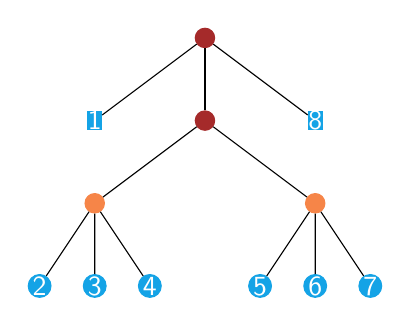
\begin{tikzpicture} [scale = 0.7,level 1/.style = {sibling distance = 2cm, level distance = 1.5cm},					  
		level 2/.style = {sibling distance = 4cm, level distance = 1.5cm},
		level 3/.style = {sibling distance = 1cm, level distance = 1.5cm}]
		\node [deep] {}
		 child{node [digit] {1} 	
		      }
		 child{node [deep] {}
		 		child{node [node] {}
		 				child{node [leaf] {2}}
		 				child{node [leaf] {3}}
		 				child{node [leaf] {4}}
		 			}
			 	child{node [node] {}
		 				child{node [leaf] {5}} 
		 				child{node [leaf] {6}}
		 				child{node [leaf] {7}}
		 			}
		 	 } 
		 child{node [digit] {8}	
		      };
	\end{tikzpicture}
}
\qquad
\subfloat[After ViewL]
{
	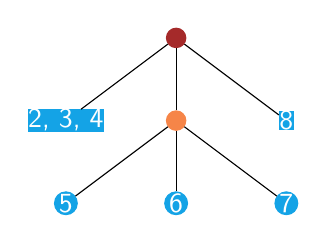
\begin{tikzpicture} [scale = 0.7,level 1/.style = {sibling distance = 2cm, level distance = 1.5cm},					  
		level 2/.style = {sibling distance = 2cm, level distance = 1.5cm},
		level 3/.style = {sibling distance = 2cm, level distance = 1.5cm}]
		\node [deep] {}
		 child{node [digit] {2, 3, 4} 	
		      }
		 child{node [node] {}
				child {node [leaf] {5}}
				child {node [leaf] {6}}
				child {node [leaf] {7}}
		}
		 child{node [digit] {8}	
		      };
	\end{tikzpicture}
}

	\caption{ViewL operation (only included the tails)}
	\label{fig:ftex4}
\end{figure}

As you can see, the composition of cons and viewL is not a no-op, but they both preserve the order of the elements.

\begin{code}
\\
\>\AgdaKeyword{mutual}\<%
\\
%
\\
\>[0]\AgdaIndent{2}{}\<[2]%
\>[2]\AgdaFunction{viewL} \AgdaSymbol{:} \AgdaSymbol{∀} \AgdaSymbol{\{}\AgdaBound{a}\AgdaSymbol{\}} \AgdaSymbol{\{}\AgdaBound{A} \AgdaSymbol{:} \AgdaPrimitiveType{Set} \AgdaBound{a}\AgdaSymbol{\}\{}\AgdaBound{V} \AgdaSymbol{:} \AgdaPrimitiveType{Set} \AgdaBound{a} \AgdaSymbol{\}}\<%
\\
\>[2]\AgdaIndent{10}{}\<[10]%
\>[10]\AgdaSymbol{⦃} \AgdaBound{mo} \AgdaSymbol{:} \AgdaRecord{Monoid} \AgdaBound{V} \AgdaSymbol{⦄}\<%
\\
\>[2]\AgdaIndent{10}{}\<[10]%
\>[10]\AgdaSymbol{⦃} \AgdaBound{m} \AgdaSymbol{:} \AgdaRecord{Measured} \AgdaBound{A} \AgdaBound{V} \AgdaSymbol{⦄}\<%
\\
\>[2]\AgdaIndent{10}{}\<[10]%
\>[10]\AgdaSymbol{\{}\AgdaBound{i} \AgdaSymbol{:} \AgdaBound{V}\AgdaSymbol{\}} \AgdaSymbol{→} \AgdaDatatype{FingerTree} \AgdaBound{A} \AgdaBound{V} \AgdaSymbol{\{}\AgdaBound{i}\AgdaSymbol{\}}\<%
\\
\>[2]\AgdaIndent{10}{}\<[10]%
\>[10]\AgdaSymbol{→} \AgdaDatatype{ViewL} \AgdaBound{A} \AgdaBound{V} \AgdaSymbol{\{}\AgdaBound{i}\AgdaSymbol{\}}\<%
\\
\>[0]\AgdaIndent{2}{}\<[2]%
\>[2]\AgdaFunction{viewL} \AgdaInductiveConstructor{Empty} \AgdaSymbol{=} \AgdaInductiveConstructor{NilL}\<%
\\
\>[0]\AgdaIndent{2}{}\<[2]%
\>[2]\AgdaFunction{viewL} \AgdaSymbol{⦃} \AgdaBound{mo} \AgdaSymbol{⦄} \AgdaSymbol{⦃} \AgdaBound{m} \AgdaSymbol{⦄} \AgdaSymbol{(}\AgdaInductiveConstructor{Single} \AgdaBound{x}\AgdaSymbol{)}\<%
\\
\>[2]\AgdaIndent{4}{}\<[4]%
\>[4]\AgdaKeyword{rewrite} \AgdaFunction{sym} \AgdaSymbol{(}\AgdaField{Monoid.ε-right} \AgdaBound{mo} \AgdaField{∥} \AgdaBound{x} \AgdaField{∥}\AgdaSymbol{)}\<%
\\
\>[2]\AgdaIndent{4}{}\<[4]%
\>[4]\AgdaSymbol{=} \AgdaInductiveConstructor{ConsL} \AgdaBound{x} \AgdaInductiveConstructor{Empty}\<%
\\
\>[0]\AgdaIndent{2}{}\<[2]%
\>[2]\AgdaFunction{viewL} \AgdaSymbol{⦃} \AgdaBound{mo} \AgdaSymbol{⦄} \AgdaSymbol{⦃} \AgdaBound{m} \AgdaSymbol{⦄} \AgdaSymbol{(}\AgdaInductiveConstructor{Deep} \AgdaBound{pr} \AgdaBound{ft} \AgdaBound{sf}\AgdaSymbol{)}\<%
\\
\>[2]\AgdaIndent{4}{}\<[4]%
\>[4]\AgdaKeyword{rewrite} \AgdaFunction{measure-digit-lemma1} \AgdaSymbol{⦃} \AgdaBound{mo} \AgdaSymbol{⦄} \AgdaSymbol{⦃} \AgdaBound{m} \AgdaSymbol{⦄} \AgdaBound{pr} \AgdaBound{ft} \AgdaBound{sf}\<%
\\
\>[2]\AgdaIndent{4}{}\<[4]%
\>[4]\AgdaSymbol{=} \AgdaInductiveConstructor{ConsL} \AgdaSymbol{(}\AgdaFunction{head-dig} \AgdaBound{pr}\AgdaSymbol{)} \AgdaSymbol{(}\AgdaFunction{deepL} \AgdaSymbol{(}\AgdaFunction{tails-dig} \AgdaBound{pr}\AgdaSymbol{)} \AgdaBound{ft} \AgdaBound{sf}\AgdaSymbol{)}\<%
\\
%
\\
\\
\\
\\
\>[0]\AgdaIndent{2}{}\<[2]%
\>[2]\AgdaFunction{deepL} \AgdaSymbol{:} \AgdaSymbol{∀} \AgdaSymbol{\{}\AgdaBound{a}\AgdaSymbol{\}\{}\AgdaBound{A} \AgdaSymbol{:} \AgdaPrimitiveType{Set} \AgdaBound{a}\AgdaSymbol{\}\{}\AgdaBound{V} \AgdaSymbol{:} \AgdaPrimitiveType{Set} \AgdaBound{a} \AgdaSymbol{\}}\<%
\\
\>[2]\AgdaIndent{8}{}\<[8]%
\>[8]\AgdaSymbol{⦃} \AgdaBound{mo} \AgdaSymbol{:} \AgdaRecord{Monoid} \AgdaBound{V} \AgdaSymbol{⦄}\<%
\\
\>[2]\AgdaIndent{8}{}\<[8]%
\>[8]\AgdaSymbol{⦃} \AgdaBound{m} \AgdaSymbol{:} \AgdaRecord{Measured} \AgdaBound{A} \AgdaBound{V} \AgdaSymbol{⦄}\<%
\\
\>[2]\AgdaIndent{8}{}\<[8]%
\>[8]\AgdaSymbol{\{}\AgdaBound{s} \AgdaSymbol{:} \AgdaBound{V}\AgdaSymbol{\}}\<%
\\
\>[2]\AgdaIndent{8}{}\<[8]%
\>[8]\AgdaSymbol{→} \AgdaSymbol{(}\AgdaBound{pr} \AgdaSymbol{:} \AgdaDatatype{Maybe} \AgdaSymbol{(}\AgdaDatatype{Digit} \AgdaBound{A}\AgdaSymbol{))}\<%
\\
\>[2]\AgdaIndent{8}{}\<[8]%
\>[8]\AgdaSymbol{→} \AgdaSymbol{(}\AgdaBound{ft} \AgdaSymbol{:} \AgdaDatatype{FingerTree} \AgdaSymbol{(}\AgdaDatatype{Node} \AgdaBound{A} \AgdaBound{V}\AgdaSymbol{)} \AgdaBound{V} \AgdaSymbol{\{}\AgdaBound{s}\AgdaSymbol{\})}\<%
\\
\>[2]\AgdaIndent{8}{}\<[8]%
\>[8]\AgdaSymbol{→} \AgdaSymbol{(}\AgdaBound{sf} \AgdaSymbol{:} \AgdaDatatype{Digit} \AgdaBound{A}\AgdaSymbol{)}\<%
\\
\>[2]\AgdaIndent{8}{}\<[8]%
\>[8]\AgdaSymbol{→} \AgdaDatatype{FingerTree} \AgdaBound{A} \AgdaBound{V} \AgdaSymbol{\{}\AgdaFunction{measure-maybe-digit} \AgdaBound{pr} \AgdaField{∙} \AgdaBound{s} \AgdaField{∙} \AgdaFunction{measure-digit} \AgdaBound{sf}\AgdaSymbol{\}}\<%
\\
\>[0]\AgdaIndent{2}{}\<[2]%
\>[2]\AgdaComment{-- deepL pr ft sf = \{!   !\}}\<%
\\
\>[0]\AgdaIndent{2}{}\<[2]%
\>[2]\AgdaFunction{deepL} \AgdaSymbol{(}\AgdaInductiveConstructor{just} \AgdaBound{x}\AgdaSymbol{)} \AgdaBound{ft} \AgdaBound{sf} \AgdaSymbol{=} \AgdaInductiveConstructor{Deep} \AgdaBound{x} \AgdaBound{ft} \AgdaBound{sf}\<%
\\
\>[0]\AgdaIndent{2}{}\<[2]%
\>[2]\AgdaFunction{deepL} \AgdaInductiveConstructor{nothing} \AgdaBound{ft} \AgdaBound{sf} \AgdaKeyword{with} \AgdaFunction{viewL} \AgdaBound{ft}\<%
\\
\>[0]\AgdaIndent{2}{}\<[2]%
\>[2]\AgdaFunction{deepL} \AgdaSymbol{⦃} \AgdaBound{mo} \AgdaSymbol{⦄} \AgdaSymbol{⦃} \AgdaBound{m} \AgdaSymbol{⦄} \AgdaInductiveConstructor{nothing} \AgdaBound{ft} \AgdaBound{sf} \AgdaSymbol{|} \AgdaInductiveConstructor{NilL}\<%
\\
\>[2]\AgdaIndent{4}{}\<[4]%
\>[4]\AgdaKeyword{rewrite} \AgdaSymbol{(}\AgdaField{Monoid.ε-left} \AgdaBound{mo}\AgdaSymbol{)} \AgdaSymbol{(}\AgdaField{ε} \AgdaField{∙} \AgdaFunction{measure-digit} \AgdaBound{sf}\AgdaSymbol{)}\<%
\\
\>[4]\AgdaIndent{10}{}\<[10]%
\>[10]\AgdaSymbol{|} \AgdaSymbol{(}\AgdaField{Monoid.ε-left} \AgdaBound{mo}\AgdaSymbol{)} \AgdaSymbol{(}\AgdaFunction{measure-digit} \AgdaBound{sf}\AgdaSymbol{)}\<%
\\
\>[0]\AgdaIndent{4}{}\<[4]%
\>[4]\AgdaSymbol{=} \AgdaFunction{toTree-dig} \AgdaBound{sf}\<%
\\
\>[0]\AgdaIndent{2}{}\<[2]%
\>[2]\AgdaFunction{deepL} \AgdaInductiveConstructor{nothing} \AgdaBound{ft} \AgdaBound{sf} \AgdaSymbol{|} \AgdaInductiveConstructor{ConsL} \AgdaSymbol{(}\AgdaInductiveConstructor{Node2} \AgdaBound{x} \AgdaBound{x₁} \AgdaBound{x₂} \AgdaBound{r}\AgdaSymbol{)} \AgdaBound{x₃}\<%
\\
\>[2]\AgdaIndent{4}{}\<[4]%
\>[4]\AgdaKeyword{rewrite} \AgdaBound{r}\<%
\\
\>[4]\AgdaIndent{10}{}\<[10]%
\>[10]\AgdaSymbol{|} \AgdaFunction{assoc-lemma3} \AgdaBound{x₁} \AgdaBound{x₂} \AgdaSymbol{(}\AgdaFunction{measure-tree} \AgdaBound{x₃}\AgdaSymbol{)} \AgdaBound{sf}\<%
\\
\>[0]\AgdaIndent{4}{}\<[4]%
\>[4]\AgdaSymbol{=} \AgdaInductiveConstructor{Deep} \AgdaSymbol{(}\AgdaInductiveConstructor{Two} \AgdaBound{x₁} \AgdaBound{x₂}\AgdaSymbol{)} \AgdaBound{x₃} \AgdaBound{sf} \AgdaComment{-- Deep (Two x₁ x₂) x₃ sf}\<%
\\
\>[0]\AgdaIndent{2}{}\<[2]%
\>[2]\AgdaFunction{deepL} \AgdaInductiveConstructor{nothing} \AgdaBound{ft} \AgdaBound{sf} \AgdaSymbol{|} \AgdaInductiveConstructor{ConsL} \AgdaSymbol{(}\AgdaInductiveConstructor{Node3} \AgdaBound{x} \AgdaBound{x₁} \AgdaBound{x₂} \AgdaBound{x₃} \AgdaBound{r}\AgdaSymbol{)} \AgdaBound{x₄}\<%
\\
\>[2]\AgdaIndent{4}{}\<[4]%
\>[4]\AgdaKeyword{rewrite} \AgdaBound{r}\<%
\\
\>[4]\AgdaIndent{10}{}\<[10]%
\>[10]\AgdaSymbol{|} \AgdaFunction{assoc-lemma4} \AgdaBound{x₁} \AgdaBound{x₂} \AgdaBound{x₃} \AgdaSymbol{(}\AgdaFunction{measure-tree} \AgdaBound{x₄}\AgdaSymbol{)} \AgdaBound{sf}\<%
\\
\>[0]\AgdaIndent{4}{}\<[4]%
\>[4]\AgdaSymbol{=} \AgdaInductiveConstructor{Deep} \AgdaSymbol{(}\AgdaInductiveConstructor{Three} \AgdaBound{x₁} \AgdaBound{x₂} \AgdaBound{x₃}\AgdaSymbol{)} \AgdaBound{x₄} \AgdaBound{sf} \AgdaComment{-- Deep (Three x₁ x₂ x₃) x₄ sf}\<%
\\
\end{code}

\subsection{Proving Correctness of \textit{viewL}}

We can proceed in an analogous way to the correctness of cons, by constructing an appropriate to-list conversion for views, and then proving that the list representations coincide.

%\begin{hscode}\SaveRestoreHook
%\column{B}{@{}>{\hspre}l<{\hspost}@{}}%
%\column{15}{@{}>{\hspre}l<{\hspost}@{}}%
%\column{E}{@{}>{\hspre}l<{\hspost}@{}}%
%\>[B]{}\Varid{viewL}\mathbin{-}\Varid{correct}\mathbin{:}\mathbin{∀}\{\mskip1.5mu \Varid{a}\mskip1.5mu\}\;\{\mskip1.5mu \Conid{A}\mathbin{:}\Conid{Set}\;\Varid{a}\mskip1.5mu\}\;\{\mskip1.5mu \Conid{V}\mathbin{:}\Conid{Set}\;\Varid{a}\mskip1.5mu\}{}\<[E]%
%\\
%\>[B]{}\hsindent{15}{}\<[15]%
%\>[15]{}\mathbin{⦃}\Varid{mo}\mathbin{:}\Conid{Monoid}\;\Conid{V}\mathbin{⦄}{}\<[E]%
%\\
%\>[B]{}\hsindent{15}{}\<[15]%
%\>[15]{}\mathbin{⦃}\Varid{m}\mathbin{:}\Conid{Measured}\;\Conid{A}\;\Conid{V}\mathbin{⦄}{}\<[E]%
%\\
%\>[B]{}\hsindent{15}{}\<[15]%
%\>[15]{}\mathbin{→}\{\mskip1.5mu \Varid{v}\mathbin{:}\Conid{V}\mskip1.5mu\}{}\<[E]%
%\\
%\>[B]{}\hsindent{15}{}\<[15]%
%\>[15]{}\mathbin{→}(\Varid{ft}\mathbin{:}\Conid{FingerTree}\;\Conid{A}\;\Conid{V}\;\{\mskip1.5mu \Varid{v}\mskip1.5mu\}){}\<[E]%
%\\
%\>[B]{}\hsindent{15}{}\<[15]%
%\>[15]{}\mathbin{→}(\Varid{toList}\mathbin{-}\Varid{view}\;(\Varid{viewL}\;\Varid{ft})\mathbin{≡}\Varid{toList}\mathbin{-}\Varid{ft}\;\Varid{ft}){}\<[E]%
%\ColumnHook
%\end{hscode}\resethooks

However, we stumble upon simple property that is unnecessarily hard to prove.

That is, we would like to prove that $viewL(ft)\equiv NilL \iff ft \equiv Empty$. This fact is obvious given the associated definitions. Unfortunately, \textit{Propositional Equality} cannot allow a term of this form, since for an arbitrary $\sigma \in V$, \textit{FingerTree A V} \{$\sigma$\} does not have the same type as Empty. (i.e. \textit{FingerTree A V} \{$\epsilon$\})

Changing the statement of the problem slightly to $\forall$ \textit{ft : FingerTree A V} \{$\epsilon$\} $viewL(ft) \equiv NilL \iff ft \equiv Empty$ allows the definition. However, the typechecker will get stuck in trying to pattern match on ft. The reason is that it cannot find terms in \textit{V} to satisfy the constrained indexing.

Indeed, if we try to prove this statement on a simpler version of \textit{FingerTree} that is indexed by Size \footnote{so that Empty can assume any size as long as it is smaller than its FingerTree derivatives (such as Deep sf Empty pr)}, it is a straightforward exercise: 

\begin{hscode}\SaveRestoreHook
\column{B}{@{}>{\hspre}l<{\hspost}@{}}%
\column{15}{@{}>{\hspre}l<{\hspost}@{}}%
\column{E}{@{}>{\hspre}l<{\hspost}@{}}%
\>[B]{}\Varid{view}\mathbin{-}\Varid{lemma3}\mathbin{:}\mathbin{∀}\{\mskip1.5mu \Varid{a}\mskip1.5mu\}\;\{\mskip1.5mu \Conid{A}\mathbin{:}\Conid{Set}\;\Varid{a}\mskip1.5mu\}\;\{\mskip1.5mu \Conid{V}\mathbin{:}\Conid{Set}\;\Varid{a}\mskip1.5mu\}{}\<[E]%
\\
\>[B]{}\hsindent{15}{}\<[15]%
\>[15]{}\mathbin{⦃}\Varid{mo}\mathbin{:}\Conid{Monoid}\;\Conid{V}\mathbin{⦄}{}\<[E]%
\\
\>[B]{}\hsindent{15}{}\<[15]%
\>[15]{}\mathbin{⦃}\Varid{m}\mathbin{:}\Conid{Measured}\;\Conid{A}\;\Conid{V}\mathbin{⦄}{}\<[E]%
\\
\>[B]{}\hsindent{15}{}\<[15]%
\>[15]{}\mathbin{→}(\Varid{ft}\mathbin{:}\Conid{FingerTree}\;\Conid{A}\;\Conid{V}){}\<[E]%
\\
\>[B]{}\hsindent{15}{}\<[15]%
\>[15]{}\mathbin{→}(\Varid{viewL}\;\Varid{ft}\mathbin{≡}\Conid{NilL}){}\<[E]%
\\
\>[B]{}\hsindent{15}{}\<[15]%
\>[15]{}\mathbin{→}(\Varid{ft}\mathbin{≡}\Conid{Empty}){}\<[E]%
\\
\>[B]{}\Varid{view}\mathbin{-}\Varid{lemma3}\;\Conid{Empty}\;\Varid{p}\mathrel{=}\Varid{refl}{}\<[E]%
\\
\>[B]{}\Varid{view}\mathbin{-}\Varid{lemma3}\;(\Conid{Single}\;\Varid{x})\;(){}\<[E]%
\\
\>[B]{}\Varid{view}\mathbin{-}\Varid{lemma3}\;(\Conid{Deep}\;\Varid{x}\;\Varid{x₁}\;\Varid{ft}\;\Varid{x₂})\;(){}\<[E]%
\ColumnHook
\end{hscode}\resethooks


A solution to this issue was suggested by McKinna\cite{heterogeneous_equality}, using an alternate implemenation of equality -- \textit{Heterogeneous Equality}, which works across types. 

Using heterogeneous equality, we can now write the type of the original statement in Agda, as well as pattern-match on the finger tree. However, some problems related to the \textit{with} construct resurface.

\subsection{\textit{with} and \textit{rewrite}}

The implementation abounds in use of \textit{with} and \textit{rewrite} statements. \textit{with} allows, inspired by the work of McBride and McKinna \cite{viewfromtheleft}, to pattern match on an intermediate computation. \textit{rewrite} replaces an expression on the left hand side, by making use of a supplied equality relation.

Their use could not be avoided in the implementation of operators that act on indexed data types. As part of the type checking, Agda has to unify the expected type of the result and the actual type of the result. 

\subparagraph{Example.} Consider the implementation of append on Vectors, but with a slight difference in terms of the index of the result. We return a vector of size $m + n$ instead of $n + m$. The type-checker cannot prove that  $+$ commutes, since it is not superfluous. This does not type-check.

\begin{hscode}\SaveRestoreHook
\column{B}{@{}>{\hspre}l<{\hspost}@{}}%
\column{9}{@{}>{\hspre}l<{\hspost}@{}}%
\column{E}{@{}>{\hspre}l<{\hspost}@{}}%
\>[B]{}\Varid{append}\mathbin{:}\mathbin{∀}\{\mskip1.5mu \Varid{a}\;\Varid{n}\;\Varid{m}\mskip1.5mu\}\mathbin{→}\{\mskip1.5mu \Conid{A}\mathbin{:}\Conid{Set}\;\Varid{a}\mskip1.5mu\}{}\<[E]%
\\
\>[B]{}\hsindent{9}{}\<[9]%
\>[9]{}\mathbin{→}\Conid{Vec}\;\Conid{A}\;\Varid{n}{}\<[E]%
\\
\>[B]{}\hsindent{9}{}\<[9]%
\>[9]{}\mathbin{→}\Conid{Vec}\;\Conid{A}\;\Varid{m}{}\<[E]%
\\
\>[B]{}\hsindent{9}{}\<[9]%
\>[9]{}\mathbin{→}\Conid{Vec}\;\Conid{A}\;(\Varid{m}\mathbin{+}\Varid{n}){}\<[E]%
\\
\>[B]{}\Varid{append}\;[\mskip1.5mu \mskip1.5mu]\;\Varid{ys}\mathrel{=}\Varid{ys}{}\<[E]%
\\
\>[B]{}\Varid{append}\;(\Varid{x}\mathbin{∷}\Varid{xs})\;\Varid{ys}\mathrel{=}\Varid{x}\mathbin{∷}(\Varid{append}\;\Varid{xs}\;\Varid{ys}){}\<[E]%
\ColumnHook
\end{hscode}\resethooks

The same situation arises in the proofs about correctness of the measure semantics. We have to provide the proof. Due to the nature of the \textit{Builtin.Equality} relation, I could not find a way to expand the functions appropriately, as suggested in the documentation \footnote{http://agda.readthedocs.io/en/latest/language/with-abstraction.html}


\subparagraph{Discussion about \textit{with}.}There is a number of issues related to the \textit{with} statement that I have stumbled upon.

\begin{itemize}
\item Computing terms that are hidden behind a \textit{with} statement requires recomputation of the expression present in the \textit{with} clause. In the \textit{FingerTree} case, this occurs because of the \textit{rewrite} statements present throughout the implementation of \textit{cons}, \textit{viewL}, \textit{deepL} etc. This causes a mild inconvenience by having to reiterate the same \textit{rewrite}s whenever one writes proofs about those definitions.

\item Whenever an argument of a function is hidden by a \textit{with abstraction}, the definition of that function cannot use further with statement containing the abstracted expression of the argument. This is discussed in the documentation: Ill-typed with-abstraction \footnote{https://agda.readthedocs.io/en/v2.5.2/language/with-abstraction.html} \\
This is the reason proving correctness of ViewL seemed complicated.

\item The type of terms hidden by \textit{with abstraction} is not available, as the feature of type checking in this conditions has not been implemented.

\item There are cases in which the termination-checker is confused in the presence of \textit{with}

Consider this example, where we try to append an element at the end of a list.

\begin{hscode}\SaveRestoreHook
\column{B}{@{}>{\hspre}l<{\hspost}@{}}%
\column{E}{@{}>{\hspre}l<{\hspost}@{}}%
\>[B]{}\Varid{append}\mathbin{:}\mathbin{∀}\{\mskip1.5mu \Varid{a}\mskip1.5mu\}\;\{\mskip1.5mu \Conid{A}\mathbin{:}\Conid{Set}\;\Varid{a}\mskip1.5mu\}\mathbin{→}\Conid{A}\mathbin{→}\Conid{List}\;\Conid{A}\mathbin{→}\Conid{List}\;\Conid{A}{}\<[E]%
\\
\>[B]{}\Varid{append}\;\Varid{x}\;\Varid{xs}\;\Varid{with}\;\Varid{xs}{}\<[E]%
\\
\>[B]{}\Varid{append}\;\Varid{x}\;\Varid{xs}\mid [\mskip1.5mu \mskip1.5mu]\mathrel{=}\Conid{\Conid{Data}.List}\mathbin{.}[\mskip1.5mu \Varid{x}\mskip1.5mu]{}\<[E]%
\\
\>[B]{}\Varid{append}\;\Varid{x}\;\Varid{xs}\mid \Varid{y}\mathbin{∷}\Varid{ys}\mathrel{=}\Varid{y}\mathbin{∷}\Varid{append}\;\Varid{x}\;\Varid{ys}{}\<[E]%
\ColumnHook
\end{hscode}\resethooks

\end{itemize}

Taking this issues into account, I have tried to come up with solutions to some of them. I will present them after finishing the main implementation of the Finger Tree.

I should note here that the proofs that I am making are still providing a powerful verification, since
\begin{itemize}
\item The FingerTree maintains all invariants
\item The measurement semantics are preserved an used sanely.
\end{itemize}

\subsection{Folding}

We can further implement the fold operation and show its correctness. I will only present, as an example the fold-left implementation.

On lists, foldl f s [x, y, z] = f (f (f s x) y) z. We can extend this to FingerTrees. Defining folds on \textbf{Node} and \textbf{Digit} is trivial, since they are just length constrained lists.

As a helper function, I define an operation to flatten a list of nodes: 

\begin{code}
\\
\>\AgdaFunction{flatten-list} \AgdaSymbol{:} \AgdaSymbol{∀} \AgdaSymbol{\{}\AgdaBound{a}\AgdaSymbol{\}\{}\AgdaBound{A} \AgdaSymbol{:} \AgdaPrimitiveType{Set} \AgdaBound{a}\AgdaSymbol{\}\{}\AgdaBound{V} \AgdaSymbol{:} \AgdaPrimitiveType{Set} \AgdaBound{a} \AgdaSymbol{\}}\<%
\\
\>[6]\AgdaIndent{14}{}\<[14]%
\>[14]\AgdaSymbol{⦃} \AgdaBound{mo} \AgdaSymbol{:} \AgdaRecord{Monoid} \AgdaBound{V} \AgdaSymbol{⦄}\<%
\\
\>[6]\AgdaIndent{14}{}\<[14]%
\>[14]\AgdaSymbol{⦃} \AgdaBound{m} \AgdaSymbol{:} \AgdaRecord{Measured} \AgdaBound{A} \AgdaBound{V} \AgdaSymbol{⦄}\<%
\\
\>[6]\AgdaIndent{14}{}\<[14]%
\>[14]\AgdaSymbol{→} \AgdaDatatype{List} \AgdaSymbol{(}\AgdaDatatype{Node} \AgdaBound{A} \AgdaBound{V}\AgdaSymbol{)}\<%
\\
\>[6]\AgdaIndent{14}{}\<[14]%
\>[14]\AgdaSymbol{→} \AgdaDatatype{List} \AgdaBound{A}\<%
\\
\>\AgdaFunction{flatten-list} \AgdaInductiveConstructor{[]} \AgdaSymbol{=} \AgdaInductiveConstructor{[]}\<%
\\
\>\AgdaFunction{flatten-list} \AgdaSymbol{(}\AgdaBound{x} \AgdaInductiveConstructor{∷} \AgdaBound{xs}\AgdaSymbol{)} \AgdaSymbol{=} \AgdaSymbol{(}\AgdaFunction{toList-node} \AgdaBound{x}\AgdaSymbol{)} \AgdaFunction{++} \AgdaSymbol{(}\AgdaFunction{flatten-list} \AgdaBound{xs}\AgdaSymbol{)}\<%
\\
\end{code}

We can then implement the foldl on finger trees as:

\begin{code}
\\
\>\AgdaFunction{foldl} \AgdaSymbol{:} \AgdaSymbol{∀} \AgdaSymbol{\{}\AgdaBound{a}\AgdaSymbol{\}} \AgdaSymbol{\{}\AgdaBound{A} \AgdaSymbol{:} \AgdaPrimitiveType{Set} \AgdaBound{a}\AgdaSymbol{\}} \AgdaSymbol{\{}\AgdaBound{V} \AgdaSymbol{:} \AgdaPrimitiveType{Set} \AgdaBound{a}\AgdaSymbol{\}}\<%
\\
\>[2]\AgdaIndent{8}{}\<[8]%
\>[8]\AgdaSymbol{\{}\AgdaBound{W} \AgdaSymbol{:} \AgdaPrimitiveType{Set} \AgdaBound{a}\AgdaSymbol{\}}\<%
\\
\>[2]\AgdaIndent{8}{}\<[8]%
\>[8]\AgdaSymbol{⦃} \AgdaBound{mo} \AgdaSymbol{:} \AgdaRecord{Monoid} \AgdaBound{V} \AgdaSymbol{⦄}\<%
\\
\>[2]\AgdaIndent{8}{}\<[8]%
\>[8]\AgdaSymbol{⦃} \AgdaBound{m} \AgdaSymbol{:} \AgdaRecord{Measured} \AgdaBound{A} \AgdaBound{V} \AgdaSymbol{⦄}\<%
\\
\>[2]\AgdaIndent{8}{}\<[8]%
\>[8]\AgdaSymbol{\{}\AgdaBound{s} \AgdaSymbol{:} \AgdaBound{V}\AgdaSymbol{\}}\<%
\\
\>[2]\AgdaIndent{8}{}\<[8]%
\>[8]\AgdaSymbol{→} \AgdaSymbol{(}\AgdaBound{W} \AgdaSymbol{→} \AgdaBound{A} \AgdaSymbol{→} \AgdaBound{W}\AgdaSymbol{)}\<%
\\
\>[2]\AgdaIndent{8}{}\<[8]%
\>[8]\AgdaSymbol{→} \AgdaBound{W}\<%
\\
\>[2]\AgdaIndent{8}{}\<[8]%
\>[8]\AgdaSymbol{→} \AgdaDatatype{FingerTree} \AgdaBound{A} \AgdaBound{V} \AgdaSymbol{\{}\AgdaBound{s}\AgdaSymbol{\}}\<%
\\
\>[2]\AgdaIndent{8}{}\<[8]%
\>[8]\AgdaSymbol{→} \AgdaBound{W}\<%
\\
\>\AgdaFunction{foldl} \AgdaBound{f} \AgdaBound{i} \AgdaInductiveConstructor{Empty} \AgdaSymbol{=} \AgdaBound{i}\<%
\\
\>\AgdaFunction{foldl} \AgdaBound{f} \AgdaBound{i} \AgdaSymbol{(}\AgdaInductiveConstructor{Single} \AgdaBound{e}\AgdaSymbol{)} \AgdaSymbol{=} \AgdaBound{f} \AgdaBound{i} \AgdaBound{e}\<%
\\
\>\AgdaFunction{foldl} \AgdaSymbol{\{}\AgdaArgument{W} \AgdaSymbol{=} \AgdaBound{W}\AgdaSymbol{\}} \AgdaBound{f} \AgdaBound{i} \AgdaSymbol{(}\AgdaInductiveConstructor{Deep} \AgdaBound{pr} \AgdaBound{ft} \AgdaBound{sf}\AgdaSymbol{)} \AgdaSymbol{=}\<%
\\
\>[0]\AgdaIndent{2}{}\<[2]%
\>[2]\AgdaFunction{foldl-dig} \AgdaBound{f} \AgdaSymbol{(}\AgdaFunction{foldl} \AgdaSymbol{(}\AgdaFunction{foldl-node} \AgdaBound{f}\AgdaSymbol{)} \AgdaSymbol{(}\AgdaFunction{foldl-dig} \AgdaBound{f} \AgdaBound{i} \AgdaBound{pr}\AgdaSymbol{)} \AgdaBound{ft}\AgdaSymbol{)} \AgdaBound{sf}\<%
\\
\end{code}

\subsection{Proving correctness of Fold Left}

Next, we will show that the previous implementation is sane, by seeing whether folding over a finger tree is equivalent to folding over its list representation.

\begin{code}
\\
\>\AgdaFunction{foldl-correct} \AgdaSymbol{:} \AgdaSymbol{∀} \AgdaSymbol{\{}\AgdaBound{a}\AgdaSymbol{\}} \AgdaSymbol{\{}\AgdaBound{A} \AgdaSymbol{:} \AgdaPrimitiveType{Set} \AgdaBound{a}\AgdaSymbol{\}\{}\AgdaBound{V} \AgdaSymbol{:} \AgdaPrimitiveType{Set} \AgdaBound{a}\AgdaSymbol{\}}\<%
\\
\>[2]\AgdaIndent{14}{}\<[14]%
\>[14]\AgdaSymbol{\{}\AgdaBound{W} \AgdaSymbol{:} \AgdaPrimitiveType{Set} \AgdaBound{a}\AgdaSymbol{\}}\<%
\\
\>[2]\AgdaIndent{14}{}\<[14]%
\>[14]\AgdaSymbol{⦃} \AgdaBound{mo} \AgdaSymbol{:} \AgdaRecord{Monoid} \AgdaBound{V} \AgdaSymbol{⦄}\<%
\\
\>[2]\AgdaIndent{14}{}\<[14]%
\>[14]\AgdaSymbol{⦃} \AgdaBound{m} \AgdaSymbol{:} \AgdaRecord{Measured} \AgdaBound{A} \AgdaBound{V} \AgdaSymbol{⦄}\<%
\\
\>[2]\AgdaIndent{14}{}\<[14]%
\>[14]\AgdaSymbol{→} \AgdaSymbol{\{}\AgdaBound{s} \AgdaSymbol{:} \AgdaBound{V}\AgdaSymbol{\}}\<%
\\
\>[2]\AgdaIndent{14}{}\<[14]%
\>[14]\AgdaSymbol{→} \AgdaSymbol{(}\AgdaBound{f} \AgdaSymbol{:} \AgdaBound{W} \AgdaSymbol{→} \AgdaBound{A} \AgdaSymbol{→} \AgdaBound{W}\AgdaSymbol{)}\<%
\\
\>[2]\AgdaIndent{14}{}\<[14]%
\>[14]\AgdaSymbol{→} \AgdaSymbol{(}\AgdaBound{σ} \AgdaSymbol{:} \AgdaBound{W}\AgdaSymbol{)}\<%
\\
\>[2]\AgdaIndent{14}{}\<[14]%
\>[14]\AgdaSymbol{→} \AgdaSymbol{(}\AgdaBound{ft} \AgdaSymbol{:} \AgdaDatatype{FingerTree} \AgdaBound{A} \AgdaBound{V} \AgdaSymbol{\{}\AgdaBound{s}\AgdaSymbol{\})}\<%
\\
\>[2]\AgdaIndent{14}{}\<[14]%
\>[14]\AgdaSymbol{→} \AgdaSymbol{(}\AgdaFunction{foldl} \AgdaBound{f} \AgdaBound{σ} \AgdaBound{ft} \AgdaDatatype{≡} \AgdaFunction{Data.List.foldl} \AgdaBound{f} \AgdaBound{σ} \AgdaSymbol{(}\AgdaFunction{toList-ft} \AgdaBound{ft}\AgdaSymbol{))}\<%
\\
\end{code}


Furthermore, fold-left has some interesting properties when it comes to its relation to the measurement. We can prove that if we fold over the finger tree using the \textbf{Monoid} and the \textbf{Measure}\footnote{foldfun v x = v ∙ ∥ x ∥} over which it is instantiated, we obtain the same result as the measure. This result is important as a sanity check of the measure semantics we are trying to preserve throughout the implementation:

\begin{code}
\\
\>\AgdaFunction{foldl-lemma0} \AgdaSymbol{:} \AgdaSymbol{∀} \AgdaSymbol{\{}\AgdaBound{a}\AgdaSymbol{\}} \AgdaSymbol{\{}\AgdaBound{A} \AgdaSymbol{:} \AgdaPrimitiveType{Set} \AgdaBound{a}\AgdaSymbol{\}} \AgdaSymbol{\{}\AgdaBound{V} \AgdaSymbol{:} \AgdaPrimitiveType{Set} \AgdaBound{a}\AgdaSymbol{\}}\<%
\\
\>[2]\AgdaIndent{14}{}\<[14]%
\>[14]\AgdaSymbol{⦃} \AgdaBound{mo} \AgdaSymbol{:} \AgdaRecord{Monoid} \AgdaBound{V} \AgdaSymbol{⦄}\<%
\\
\>[2]\AgdaIndent{14}{}\<[14]%
\>[14]\AgdaSymbol{⦃} \AgdaBound{m} \AgdaSymbol{:} \AgdaRecord{Measured} \AgdaBound{A} \AgdaBound{V} \AgdaSymbol{⦄}\<%
\\
\>[2]\AgdaIndent{14}{}\<[14]%
\>[14]\AgdaSymbol{→} \AgdaSymbol{\{}\AgdaBound{s} \AgdaSymbol{:} \AgdaBound{V}\AgdaSymbol{\}}\<%
\\
\>[2]\AgdaIndent{14}{}\<[14]%
\>[14]\AgdaSymbol{→} \AgdaSymbol{(}\AgdaBound{v} \AgdaSymbol{:} \AgdaBound{V}\AgdaSymbol{)}\<%
\\
\>[2]\AgdaIndent{14}{}\<[14]%
\>[14]\AgdaSymbol{→} \AgdaSymbol{(}\AgdaBound{ft} \AgdaSymbol{:} \AgdaDatatype{FingerTree} \AgdaBound{A} \AgdaBound{V} \AgdaSymbol{\{}\AgdaBound{s}\AgdaSymbol{\})}\<%
\\
\>[2]\AgdaIndent{14}{}\<[14]%
\>[14]\AgdaSymbol{→} \AgdaSymbol{(}\AgdaFunction{foldl} \AgdaFunction{foldfun} \AgdaBound{v} \AgdaBound{ft} \AgdaDatatype{≡} \AgdaBound{v} \AgdaField{∙} \AgdaBound{s}\AgdaSymbol{)}\<%
\\
\end{code}

\subsection{Splitting}

Splitting is an extension of the ViewL paradigm, by allowing extraction of elements arbitrarily deep in the FingerTree. It consists of a left side, a middle element, and a right side.\footnote{the sides are correct FingerTrees}

The same issues occur, as it was the case of viewL. I have tried in this implementation to keep the usage of \textit{with} at a minimum. This turned out to be a very difficult task, so correctness of this method can only be provided in terms of its measure, which is being taken care of by the indexing.

The split is done over a boolean predicate, $p \in V \to Bool$ and a starting value, $i \in V$. The method iterates through the FingerTree, element by element, at each step increasing $i$ by the measure of the current element, $\Vert x \Vert$. The split is done when the value of the predicate $p(i) = True$, and the element at which this change occurs becomes the middle.


As with ViewL, we create an additional data-type that will represent the result. It is indexed by the measurement, ensuring correctness.

\begin{code}
\\
\>\AgdaKeyword{data} \AgdaDatatype{Split-d} \AgdaSymbol{\{}\AgdaBound{a}\AgdaSymbol{\}} \AgdaSymbol{(}\AgdaBound{A} \AgdaSymbol{:} \AgdaPrimitiveType{Set} \AgdaBound{a}\AgdaSymbol{)} \AgdaSymbol{(}\AgdaBound{V} \AgdaSymbol{:} \AgdaPrimitiveType{Set} \AgdaBound{a}\AgdaSymbol{)}\<%
\\
\>[2]\AgdaIndent{12}{}\<[12]%
\>[12]\AgdaSymbol{⦃} \AgdaBound{mo} \AgdaSymbol{:} \AgdaRecord{Monoid} \AgdaBound{V} \AgdaSymbol{⦄}\<%
\\
\>[2]\AgdaIndent{12}{}\<[12]%
\>[12]\AgdaSymbol{⦃} \AgdaBound{m} \AgdaSymbol{:} \AgdaRecord{Measured} \AgdaBound{A} \AgdaBound{V} \AgdaSymbol{⦄} \AgdaSymbol{:}\<%
\\
\>[2]\AgdaIndent{12}{}\<[12]%
\>[12]\AgdaSymbol{\{}\AgdaBound{μ} \AgdaSymbol{:} \AgdaBound{V}\AgdaSymbol{\}} \AgdaSymbol{→} \AgdaPrimitiveType{Set} \AgdaBound{a} \AgdaKeyword{where}\<%
\\
\>[0]\AgdaIndent{2}{}\<[2]%
\>[2]\AgdaInductiveConstructor{split-d} \AgdaSymbol{:} \AgdaSymbol{∀} \AgdaSymbol{\{}\AgdaBound{μ₁} \AgdaSymbol{:} \AgdaBound{V}\AgdaSymbol{\}} \AgdaSymbol{\{}\AgdaBound{μ₂} \AgdaSymbol{:} \AgdaBound{V}\AgdaSymbol{\}}\<%
\\
\>[2]\AgdaIndent{10}{}\<[10]%
\>[10]\AgdaSymbol{→} \AgdaSymbol{(}\AgdaDatatype{FingerTree} \AgdaBound{A} \AgdaBound{V} \AgdaSymbol{\{}\AgdaBound{μ₁}\AgdaSymbol{\})} \<[35]%
\>[35]\AgdaComment{-- left side}\<%
\\
\>[2]\AgdaIndent{10}{}\<[10]%
\>[10]\AgdaSymbol{→} \AgdaSymbol{(}\AgdaBound{x} \AgdaSymbol{:} \AgdaBound{A}\AgdaSymbol{)} \<[35]%
\>[35]\AgdaComment{-- middle}\<%
\\
\>[2]\AgdaIndent{10}{}\<[10]%
\>[10]\AgdaSymbol{→} \AgdaSymbol{(}\AgdaDatatype{FingerTree} \AgdaBound{A} \AgdaBound{V} \AgdaSymbol{\{}\AgdaBound{μ₂}\AgdaSymbol{\})} \<[35]%
\>[35]\AgdaComment{-- right side}\<%
\\
\>[2]\AgdaIndent{10}{}\<[10]%
\>[10]\AgdaSymbol{→} \AgdaDatatype{Split-d} \AgdaBound{A} \AgdaBound{V} \AgdaSymbol{\{}\AgdaBound{μ₁} \AgdaField{∙} \AgdaField{∥} \AgdaBound{x} \AgdaField{∥} \AgdaField{∙} \AgdaBound{μ₂}\AgdaSymbol{\}}\<%
\\
\end{code}

Since this implementation is long a full of necessary proofs about the types, I will only provide the most important snippets.

\subparagraph{Discussion} This implementation was also made difficult because of the partiality of the function in the original paper. Wrapping things in the Maybe monad can confuse the type-checker at times.

\subparagraph{The main procedure} pattern matches on the constructors for the Finger Tree provided as argument. Notice that the typing already maintains the invariant.

\begin{code}
\\
\>[0]\AgdaIndent{2}{}\<[2]%
\>[2]\AgdaFunction{split-Tree} \AgdaSymbol{:} \AgdaSymbol{∀} \AgdaSymbol{\{}\AgdaBound{a}\AgdaSymbol{\}} \AgdaSymbol{\{}\AgdaBound{A} \AgdaSymbol{:} \AgdaPrimitiveType{Set} \AgdaBound{a}\AgdaSymbol{\}} \AgdaSymbol{\{}\AgdaBound{V} \AgdaSymbol{:} \AgdaPrimitiveType{Set} \AgdaBound{a}\AgdaSymbol{\}}\<%
\\
\>[2]\AgdaIndent{14}{}\<[14]%
\>[14]\AgdaSymbol{⦃} \AgdaBound{mo} \AgdaSymbol{:} \AgdaRecord{Monoid} \AgdaBound{V} \AgdaSymbol{⦄}\<%
\\
\>[2]\AgdaIndent{14}{}\<[14]%
\>[14]\AgdaSymbol{⦃} \AgdaBound{m} \AgdaSymbol{:} \AgdaRecord{Measured} \AgdaBound{A} \AgdaBound{V} \AgdaSymbol{⦄}\<%
\\
\>[2]\AgdaIndent{14}{}\<[14]%
\>[14]\AgdaSymbol{\{}\AgdaBound{μ} \AgdaSymbol{:} \AgdaBound{V}\AgdaSymbol{\}} \AgdaComment{-- type class information}\<%
\\
\>[2]\AgdaIndent{14}{}\<[14]%
\>[14]\AgdaSymbol{→} \AgdaSymbol{(}\AgdaBound{p} \AgdaSymbol{:} \AgdaBound{V} \AgdaSymbol{→} \AgdaDatatype{Bool}\AgdaSymbol{)} \AgdaSymbol{→} \AgdaSymbol{(}\AgdaBound{i} \AgdaSymbol{:} \AgdaBound{V}\AgdaSymbol{)} \AgdaComment{-- predicate and inital value}\<%
\\
\>[2]\AgdaIndent{14}{}\<[14]%
\>[14]\AgdaSymbol{→} \AgdaSymbol{(}\AgdaBound{ft} \AgdaSymbol{:} \AgdaDatatype{FingerTree} \AgdaBound{A} \AgdaBound{V} \AgdaSymbol{\{}\AgdaBound{μ}\AgdaSymbol{\})} \AgdaComment{-- argument}\<%
\\
\>[2]\AgdaIndent{14}{}\<[14]%
\>[14]\AgdaSymbol{→} \AgdaDatatype{Maybe} \AgdaSymbol{(}\AgdaDatatype{Split-d} \AgdaBound{A} \AgdaBound{V} \AgdaSymbol{\{}\AgdaBound{μ}\AgdaSymbol{\})}\<%
\\
\>[0]\AgdaIndent{2}{}\<[2]%
\>[2]\AgdaFunction{split-Tree} \AgdaBound{p} \AgdaBound{i} \AgdaInductiveConstructor{Empty}\<%
\\
\>[2]\AgdaIndent{4}{}\<[4]%
\>[4]\AgdaSymbol{=} \AgdaInductiveConstructor{nothing} \<[15]%
\>[15]\AgdaComment{-- cannot split an empty tree}\<%
\\
\>[0]\AgdaIndent{2}{}\<[2]%
\>[2]\AgdaFunction{split-Tree} \AgdaBound{p} \AgdaBound{i} \AgdaSymbol{(}\AgdaInductiveConstructor{Single} \AgdaBound{e}\AgdaSymbol{)}\<%
\\
\>[2]\AgdaIndent{4}{}\<[4]%
\>[4]\AgdaSymbol{=} \AgdaInductiveConstructor{just} \AgdaSymbol{(}\AgdaFunction{split-Tree-single} \AgdaBound{p} \AgdaBound{i} \AgdaBound{e}\AgdaSymbol{)} \AgdaComment{-- superfluous case}\<%
\\
\>[0]\AgdaIndent{2}{}\<[2]%
\>[2]\AgdaFunction{split-Tree} \AgdaBound{p} \AgdaBound{i} \AgdaSymbol{(}\AgdaInductiveConstructor{Deep} \AgdaBound{pr} \AgdaBound{ft} \AgdaBound{sf}\AgdaSymbol{)}\<%
\\
\>[2]\AgdaIndent{4}{}\<[4]%
\>[4]\AgdaSymbol{=} \AgdaInductiveConstructor{just} \AgdaSymbol{(}\AgdaFunction{split-Tree-if} \AgdaBound{p} \AgdaBound{i} \AgdaBound{pr} \AgdaBound{ft} \AgdaBound{sf} \AgdaFunction{vpr} \AgdaInductiveConstructor{refl} \AgdaFunction{vft} \AgdaInductiveConstructor{refl}\AgdaSymbol{)} \AgdaComment{-- recursive case}\<%
\\
\>[2]\AgdaIndent{4}{}\<[4]%
\>[4]\AgdaKeyword{where}\<%
\\
\>[4]\AgdaIndent{6}{}\<[6]%
\>[6]\AgdaFunction{vpr} \AgdaSymbol{=} \AgdaBound{p} \AgdaSymbol{(}\AgdaBound{i} \AgdaField{∙} \AgdaSymbol{(}\AgdaFunction{measure-digit} \AgdaBound{pr}\AgdaSymbol{))}\<%
\\
\>[4]\AgdaIndent{6}{}\<[6]%
\>[6]\AgdaFunction{vft} \AgdaSymbol{=} \AgdaBound{p} \AgdaSymbol{((}\AgdaBound{i} \AgdaField{∙} \AgdaFunction{measure-digit} \AgdaBound{pr}\AgdaSymbol{)} \AgdaField{∙} \AgdaFunction{measure-tree} \AgdaBound{ft}\AgdaSymbol{)}\<%
\\
%
\end{code}


The \textbf{split-Tree-if} function splits the computation in three cases, depending where the predicate changes to \textit{True}. This could happen after the during the prefix \textbf{pr}, during the nested finger tree \textbf{ft} or during the suffix \textbf{sf} 

\begin{code}
\\
\\
\>[0]\AgdaIndent{2}{}\<[2]%
\>[2]\AgdaFunction{split-Tree-if} \AgdaSymbol{:} \AgdaSymbol{∀} \AgdaSymbol{\{}\AgdaBound{a}\AgdaSymbol{\}} \AgdaSymbol{\{}\AgdaBound{A} \AgdaSymbol{:} \AgdaPrimitiveType{Set} \AgdaBound{a}\AgdaSymbol{\}} \AgdaSymbol{\{}\AgdaBound{V} \AgdaSymbol{:} \AgdaPrimitiveType{Set} \AgdaBound{a}\AgdaSymbol{\}}\<%
\\
\>[2]\AgdaIndent{16}{}\<[16]%
\>[16]\AgdaSymbol{⦃} \AgdaBound{mo} \AgdaSymbol{:} \AgdaRecord{Monoid} \AgdaBound{V} \AgdaSymbol{⦄}\<%
\\
\>[2]\AgdaIndent{16}{}\<[16]%
\>[16]\AgdaSymbol{⦃} \AgdaBound{m} \AgdaSymbol{:} \AgdaRecord{Measured} \AgdaBound{A} \AgdaBound{V} \AgdaSymbol{⦄}\<%
\\
\>[2]\AgdaIndent{16}{}\<[16]%
\>[16]\AgdaSymbol{\{}\AgdaBound{μ} \AgdaSymbol{:} \AgdaBound{V}\AgdaSymbol{\}}\<%
\\
\>[2]\AgdaIndent{16}{}\<[16]%
\>[16]\AgdaSymbol{→} \AgdaSymbol{(}\AgdaBound{p} \AgdaSymbol{:} \AgdaBound{V} \AgdaSymbol{→} \AgdaDatatype{Bool}\AgdaSymbol{)} \AgdaSymbol{→} \AgdaSymbol{(}\AgdaBound{i} \AgdaSymbol{:} \AgdaBound{V}\AgdaSymbol{)} \<[44]%
\>[44]\AgdaComment{-- predicate and initial value}\<%
\\
\>[2]\AgdaIndent{16}{}\<[16]%
\>[16]\AgdaSymbol{→} \AgdaSymbol{(}\AgdaBound{pr} \AgdaSymbol{:} \AgdaDatatype{Digit} \AgdaBound{A}\AgdaSymbol{)} \<[45]%
\>[45]\AgdaComment{-- prefix}\<%
\\
\>[2]\AgdaIndent{16}{}\<[16]%
\>[16]\AgdaSymbol{→} \AgdaSymbol{(}\AgdaBound{ft} \AgdaSymbol{:} \AgdaDatatype{FingerTree} \AgdaSymbol{(}\AgdaDatatype{Node} \AgdaBound{A} \AgdaBound{V}\AgdaSymbol{)} \AgdaBound{V} \AgdaSymbol{\{}\AgdaBound{μ}\AgdaSymbol{\})} \AgdaComment{-- nested tree}\<%
\\
\>[2]\AgdaIndent{16}{}\<[16]%
\>[16]\AgdaSymbol{→} \AgdaSymbol{(}\AgdaBound{sf} \AgdaSymbol{:} \AgdaDatatype{Digit} \AgdaBound{A}\AgdaSymbol{)} \<[43]%
\>[43]\AgdaComment{-- suffix}\<%
\\
\>[2]\AgdaIndent{16}{}\<[16]%
\>[16]\AgdaSymbol{→} \AgdaSymbol{(}\AgdaBound{vpr} \AgdaSymbol{:} \AgdaDatatype{Bool}\AgdaSymbol{)} \<[43]%
\>[43]\AgdaComment{-- value of predicate after prefix}\<%
\\
\>[2]\AgdaIndent{16}{}\<[16]%
\>[16]\AgdaSymbol{→} \AgdaSymbol{(}\AgdaBound{vpr} \AgdaDatatype{≡} \AgdaBound{p} \AgdaSymbol{(}\AgdaBound{i} \AgdaField{∙} \AgdaFunction{measure-digit} \AgdaBound{pr}\AgdaSymbol{))} \AgdaComment{-- correctness check}\<%
\\
\>[2]\AgdaIndent{16}{}\<[16]%
\>[16]\AgdaSymbol{→} \AgdaSymbol{(}\AgdaBound{vft} \AgdaSymbol{:} \AgdaDatatype{Bool}\AgdaSymbol{)} \<[43]%
\>[43]\AgdaComment{-- value of predicate after tree}\<%
\\
\>[2]\AgdaIndent{16}{}\<[16]%
\>[16]\AgdaSymbol{→} \AgdaSymbol{(}\AgdaBound{vft} \AgdaDatatype{≡} \AgdaBound{p} \AgdaSymbol{((}\AgdaBound{i} \AgdaField{∙} \AgdaFunction{measure-digit} \AgdaBound{pr}\AgdaSymbol{)} \AgdaField{∙} \AgdaSymbol{(}\AgdaFunction{measure-tree} \AgdaBound{ft}\AgdaSymbol{)))} \AgdaComment{-- check}\<%
\\
\>[2]\AgdaIndent{16}{}\<[16]%
\>[16]\AgdaSymbol{→} \AgdaDatatype{Split-d} \AgdaBound{A} \AgdaBound{V} \AgdaSymbol{\{(}\AgdaFunction{measure-digit} \AgdaBound{pr}\AgdaSymbol{)} \AgdaField{∙} \AgdaBound{μ} \AgdaField{∙} \AgdaSymbol{(}\AgdaFunction{measure-digit} \AgdaBound{sf}\AgdaSymbol{)\}}\<%
\\
\>[0]\AgdaIndent{2}{}\<[2]%
\>[2]\AgdaFunction{split-Tree-if} \AgdaBound{p} \AgdaBound{i} \AgdaBound{pr} \AgdaBound{ft} \AgdaBound{sf} \AgdaInductiveConstructor{false} \AgdaBound{pr1} \AgdaInductiveConstructor{false} \AgdaBound{pr2}\<%
\\
\>[2]\AgdaIndent{4}{}\<[4]%
\>[4]\AgdaSymbol{=} \AgdaFunction{split-Tree2} \AgdaBound{p} \AgdaSymbol{((}\AgdaBound{i} \AgdaField{∙} \AgdaFunction{measure-digit} \AgdaBound{pr}\AgdaSymbol{)} \AgdaField{∙} \AgdaSymbol{(}\AgdaFunction{measure-tree} \AgdaBound{ft}\AgdaSymbol{))} \AgdaBound{pr} \AgdaBound{ft} \AgdaBound{sf}\<%
\\
\>[2]\AgdaIndent{4}{}\<[4]%
\>[4]\AgdaComment{-- case2 : predicate becomes true in suffix or not at all}\<%
\\
\>[0]\AgdaIndent{2}{}\<[2]%
\>[2]\AgdaFunction{split-Tree-if} \AgdaBound{p} \AgdaBound{i} \AgdaBound{pr} \AgdaBound{ft} \AgdaBound{sf} \AgdaInductiveConstructor{false} \AgdaBound{pr1} \AgdaInductiveConstructor{true} \AgdaBound{pr2}\<%
\\
\>[2]\AgdaIndent{4}{}\<[4]%
\>[4]\AgdaSymbol{=} \AgdaFunction{split-Tree3} \AgdaBound{p} \AgdaBound{i} \AgdaBound{pr} \AgdaBound{ft} \AgdaBound{sf} \AgdaSymbol{(}\AgdaFunction{sym} \AgdaBound{pr1}\AgdaSymbol{)} \AgdaSymbol{(}\AgdaFunction{sym} \AgdaBound{pr2}\AgdaSymbol{)}\<%
\\
\>[2]\AgdaIndent{4}{}\<[4]%
\>[4]\AgdaComment{-- case3 : predicate becomes true in tree}\<%
\\
\>[0]\AgdaIndent{2}{}\<[2]%
\>[2]\AgdaFunction{split-Tree-if} \AgdaBound{p} \AgdaBound{i} \AgdaBound{pr} \AgdaBound{ft} \AgdaBound{sf} \AgdaInductiveConstructor{true} \AgdaBound{pr1} \AgdaBound{vft} \AgdaBound{pr2}\<%
\\
\>[2]\AgdaIndent{4}{}\<[4]%
\>[4]\AgdaSymbol{=} \AgdaFunction{split-Tree1} \AgdaBound{p} \AgdaBound{i} \AgdaBound{pr} \AgdaBound{ft} \AgdaBound{sf}\<%
\\
\>[2]\AgdaIndent{4}{}\<[4]%
\>[4]\AgdaComment{-- case1 : predicate becomes true in prefix}\<%
\\
\end{code}

The full implementation requires more advanced agda syntax, as well as the implementation of the ViewR and deepR. It is present in the Appendix.

\section{Other recursive definitions}

The difficulties of writing a recursive function that outputs a value of a type dependent on one of the arguments become apparent with the example of reversing.

The implementation of reverse is straight-forward in terms of folding. We could, ideally, reverse a FingerTree simply by 

\begin{center}
\textit{reverse ft = foldl \_▷\_ Empty ft}
\end{center}

However, declaring this in this form is impossible because of two resons:

\begin{itemize}
\item \textbf{\_▷\_} is a dependent function, incompatible with our definition of \textbf{foldl} \footnote{https://nicolaspouillard.fr/publis/explore-iso.pdf}

It is possible to implement an analogous dependent version of foldl. Doing so will however yield a specific solution to the reverse function of the FingerTree.
Transforming the FingerTree first to a list and then folding it is another strategy for achieving a similar result. Unfortunately, this will incur an unnecessary computational cost.
 
\item The index of the output FingerTree depends on the argument as well, yielding in this case 
\begin{center}
measure-ft (reverse ft) = foldl foldfun $\epsilon$ (List.reverse (toList-ft ft))
\end{center}
\end{itemize}

In this example, the cost of dependent types becomes very clear, and can be avoided by providing a non-dependent interface.

\subsection{Reverse}

The non-dependent interface is constructed through a dependent pair. The function \textbf{pack} makes the transformation, and the \textbf{cons-pair} is simply the extension of \textbf{cons} to the pair.
\begin{code}
\\
\>\AgdaFunction{reverse-ft} \AgdaSymbol{:} \AgdaSymbol{∀} \AgdaSymbol{\{}\AgdaBound{a}\AgdaSymbol{\}} \AgdaSymbol{\{}\AgdaBound{A} \AgdaSymbol{:} \AgdaPrimitiveType{Set} \AgdaBound{a}\AgdaSymbol{\}} \AgdaSymbol{\{}\AgdaBound{V} \AgdaSymbol{:} \AgdaPrimitiveType{Set} \AgdaBound{a}\AgdaSymbol{\}}\<%
\\
\>[2]\AgdaIndent{10}{}\<[10]%
\>[10]\AgdaSymbol{⦃} \AgdaBound{mo} \AgdaSymbol{:} \AgdaRecord{Monoid} \AgdaBound{V} \AgdaSymbol{⦄}\<%
\\
\>[2]\AgdaIndent{10}{}\<[10]%
\>[10]\AgdaSymbol{⦃} \AgdaBound{m} \AgdaSymbol{:} \AgdaRecord{Measured} \AgdaBound{A} \AgdaBound{V} \AgdaSymbol{⦄}\<%
\\
\>[2]\AgdaIndent{10}{}\<[10]%
\>[10]\AgdaSymbol{→} \AgdaSymbol{(}\AgdaRecord{Σ} \AgdaBound{V} \AgdaSymbol{(λ} \AgdaBound{v} \AgdaSymbol{→} \AgdaDatatype{FingerTree} \AgdaBound{A} \AgdaBound{V} \AgdaSymbol{\{}\AgdaBound{v}\AgdaSymbol{\}))}\<%
\\
\>[2]\AgdaIndent{10}{}\<[10]%
\>[10]\AgdaSymbol{→} \AgdaSymbol{(}\AgdaRecord{Σ} \AgdaBound{V} \AgdaSymbol{(λ} \AgdaBound{v} \AgdaSymbol{→} \AgdaDatatype{FingerTree} \AgdaBound{A} \AgdaBound{V} \AgdaSymbol{\{}\AgdaBound{v}\AgdaSymbol{\}))}\<%
\\
\>\AgdaFunction{reverse-ft} \AgdaSymbol{\{}\AgdaBound{a}\AgdaSymbol{\}} \AgdaSymbol{\{}\AgdaBound{A}\AgdaSymbol{\}} \AgdaSymbol{\{}\AgdaBound{V}\AgdaSymbol{\}} \AgdaBound{pair} \AgdaSymbol{=}\<%
\\
\>[0]\AgdaIndent{2}{}\<[2]%
\>[2]\AgdaFunction{foldl-pair} \AgdaFunction{cons-pair} \AgdaSymbol{(}\AgdaFunction{pack-ft} \AgdaSymbol{\{}\AgdaArgument{A} \AgdaSymbol{=} \AgdaBound{A}\AgdaSymbol{\}} \AgdaSymbol{\{}\AgdaArgument{V} \AgdaSymbol{=} \AgdaBound{V}\AgdaSymbol{\}} \AgdaInductiveConstructor{Empty}\AgdaSymbol{)} \AgdaBound{pair}\<%
\\
%
\end{code} 

Note that this implementation no longer constrains the result to the argument. The only verified property of this is that the result will itself be a correctly constructed FingerTree.

\section{Random Access Sequences}

By proper instantiation of the measurement function and monoid, we can specialize the Finger Tree to various data structures. The first suggested on is the Random Access Sequence.

The measurement function will assign the value of 1 to any element, and the monoid is simply that of the natural numbers with addition. For convenience, I will wrap both the size and the entries is special types, to aid with the use of instance arguments.

\subsection{SizeW and Entry}

The \textit{SizeW} is simply a wrapper around \textit{Nat}\footnote{for compatibility with the rest of the implementation, I had to assign an arbitrary universe level \textit{a}} 


\begin{code}
\\
\>[0]\AgdaIndent{2}{}\<[2]%
\>[2]\AgdaKeyword{data} \AgdaDatatype{SizeW} \AgdaSymbol{\{}\AgdaBound{a}\AgdaSymbol{\}} \AgdaSymbol{:} \AgdaPrimitiveType{Set} \AgdaBound{a} \<[26]%
\>[26]\AgdaKeyword{where}\<%
\\
\>[2]\AgdaIndent{4}{}\<[4]%
\>[4]\AgdaInductiveConstructor{size} \AgdaSymbol{:} \AgdaSymbol{∀} \AgdaSymbol{(}\AgdaBound{n} \AgdaSymbol{:} \AgdaDatatype{ℕ}\AgdaSymbol{)} \AgdaSymbol{→} \AgdaDatatype{SizeW} \AgdaSymbol{\{}\AgdaBound{a}\AgdaSymbol{\}}\<%
\\
\>[0]\AgdaIndent{2}{}\<[2]%
\>[2]\AgdaFunction{ε} \AgdaSymbol{:} \AgdaSymbol{∀} \AgdaSymbol{\{}\AgdaBound{a} \AgdaSymbol{:} \AgdaPostulate{Level}\AgdaSymbol{\}} \AgdaSymbol{→} \AgdaDatatype{SizeW} \AgdaSymbol{\{}\AgdaBound{a}\AgdaSymbol{\}}\<%
\\
\>[0]\AgdaIndent{2}{}\<[2]%
\>[2]\AgdaFunction{ε} \AgdaSymbol{=} \AgdaInductiveConstructor{size} \AgdaNumber{0}\<%
\\
%
\\
\>[0]\AgdaIndent{2}{}\<[2]%
\>[2]\AgdaFunction{\_∙\_} \AgdaSymbol{:} \<[9]%
\>[9]\AgdaSymbol{∀} \AgdaSymbol{\{}\AgdaBound{a}\AgdaSymbol{\}} \AgdaSymbol{→} \AgdaDatatype{SizeW} \AgdaSymbol{\{}\AgdaBound{a}\AgdaSymbol{\}} \AgdaSymbol{→} \AgdaDatatype{SizeW} \AgdaSymbol{\{}\AgdaBound{a}\AgdaSymbol{\}} \AgdaSymbol{→} \AgdaDatatype{SizeW} \AgdaSymbol{\{}\AgdaBound{a}\AgdaSymbol{\}}\<%
\\
\>[0]\AgdaIndent{2}{}\<[2]%
\>[2]\AgdaInductiveConstructor{size} \AgdaBound{n} \AgdaFunction{∙} \AgdaInductiveConstructor{size} \AgdaBound{m} \AgdaSymbol{=} \AgdaInductiveConstructor{size} \AgdaSymbol{(}\AgdaBound{n} \AgdaPrimitive{+} \AgdaBound{m}\AgdaSymbol{)}\<%
\\
\end{code}

The properties of the \textit{Nat} carries directly to\textit{SizeW}, so that we can populate a \textit{Monoid SizeW}

\begin{code}
\\
\>[0]\AgdaIndent{2}{}\<[2]%
\>[2]\AgdaKeyword{instance} \AgdaFunction{size-monoid} \AgdaSymbol{:} \AgdaSymbol{∀} \AgdaSymbol{\{}\AgdaBound{a}\AgdaSymbol{\}} \AgdaSymbol{→} \AgdaRecord{Monoid} \AgdaSymbol{(}\AgdaDatatype{SizeW} \AgdaSymbol{\{}\AgdaBound{a}\AgdaSymbol{\})}\<%
\\
\>[0]\AgdaIndent{2}{}\<[2]%
\>[2]\AgdaFunction{size-monoid} \AgdaSymbol{=} \AgdaInductiveConstructor{monoid} \AgdaFunction{ε} \AgdaFunction{\_∙\_} \AgdaFunction{ε∙} \AgdaFunction{∙ε} \AgdaFunction{∙-assoc} \AgdaDatatype{\_<ᵗ\_}\<%
\\
\end{code}

\textit{Entry A} is a wrapper around elements of type A, given by the constructor \textit{entry}.


\begin{code}
\\
\>[0]\AgdaIndent{2}{}\<[2]%
\>[2]\AgdaFunction{measure} \AgdaSymbol{:} \AgdaSymbol{∀} \AgdaSymbol{\{}\AgdaBound{a}\AgdaSymbol{\}\{}\AgdaBound{A} \AgdaSymbol{:} \AgdaPrimitiveType{Set} \AgdaBound{a}\AgdaSymbol{\}} \AgdaSymbol{→} \AgdaSymbol{(}\AgdaBound{x} \AgdaSymbol{:} \AgdaDatatype{Entry} \AgdaBound{A}\AgdaSymbol{)} \AgdaSymbol{→} \AgdaDatatype{SizeW} \AgdaSymbol{\{}\AgdaBound{a}\AgdaSymbol{\}}\<%
\\
\>[0]\AgdaIndent{2}{}\<[2]%
\>[2]\AgdaFunction{measure} \AgdaBound{x} \AgdaSymbol{=} \AgdaInductiveConstructor{SizeW.size} \AgdaNumber{1}\<%
\\
%
\\
\>[0]\AgdaIndent{2}{}\<[2]%
\>[2]\AgdaKeyword{instance} \AgdaFunction{entry-measure} \AgdaSymbol{:} \AgdaSymbol{∀\{}\AgdaBound{a}\AgdaSymbol{\}\{}\AgdaBound{A} \AgdaSymbol{:} \AgdaPrimitiveType{Set} \AgdaBound{a}\AgdaSymbol{\}} \AgdaSymbol{→} \AgdaRecord{Measured} \AgdaSymbol{(}\AgdaDatatype{Entry} \AgdaBound{A}\AgdaSymbol{)} \AgdaDatatype{SizeW}\<%
\\
\>[0]\AgdaIndent{2}{}\<[2]%
\>[2]\AgdaFunction{entry-measure} \AgdaSymbol{=} \AgdaInductiveConstructor{measured} \AgdaFunction{measure}\<%
\end{code}

\subsection{Seq Instance}

The Sequence instance is simply an alias for a Finger Tree, instantiated with an arbitrarily typed Entry and the SizeW monoid.

\begin{code}
\\
\>[0]\AgdaIndent{4}{}\<[4]%
\>[4]\AgdaFunction{Seq} \AgdaSymbol{:} \AgdaSymbol{∀} \AgdaSymbol{\{}\AgdaBound{a}\AgdaSymbol{\}(}\AgdaBound{A} \AgdaSymbol{:} \AgdaPrimitiveType{Set} \AgdaBound{a}\AgdaSymbol{)} \AgdaBound{SizeW} \AgdaSymbol{→} \AgdaPrimitiveType{Set} \AgdaBound{a}\<%
\\
\>[0]\AgdaIndent{4}{}\<[4]%
\>[4]\AgdaFunction{Seq} \AgdaSymbol{\{}\AgdaBound{a}\AgdaSymbol{\}} \AgdaBound{A} \AgdaBound{s} \AgdaSymbol{=} \AgdaDatatype{FingerTree} \AgdaSymbol{(}\AgdaDatatype{Entry} \AgdaBound{A}\AgdaSymbol{)} \AgdaSymbol{(}\AgdaDatatype{SizeW} \AgdaSymbol{\{}\AgdaBound{a}\AgdaSymbol{\})} \AgdaSymbol{\{}\AgdaBound{s}\AgdaSymbol{\}}\<%
\\
\end{code}

\paragraph{Retrieving the nth element} \mbox{} \\ 
The naive implementation would simply call the \textit{viewL} n times, yielding an amortized linear cost.

However, we can find an $\mathcal{O}(log(n))$ implementation, by using \textit{split}. The predicate checks whether the current value is smaller than n, and we will start iterating from 0.

\begin{code}
\>[0]\AgdaIndent{4}{}\<[4]%
\>[4]\AgdaFunction{\_!\_} \AgdaSymbol{:} \AgdaSymbol{∀} \AgdaSymbol{\{}\AgdaBound{a}\AgdaSymbol{\}\{}\AgdaBound{A} \AgdaSymbol{:} \AgdaPrimitiveType{Set} \AgdaBound{a}\AgdaSymbol{\}\{}\AgdaBound{s} \AgdaSymbol{:} \AgdaDatatype{SizeW}\AgdaSymbol{\}} \AgdaSymbol{→} \AgdaFunction{Seq} \AgdaBound{A} \AgdaBound{s} \AgdaSymbol{→} \AgdaDatatype{ℕ} \AgdaSymbol{→} \AgdaDatatype{Maybe} \AgdaBound{A}\<%
\\
\>[0]\AgdaIndent{4}{}\<[4]%
\>[4]\AgdaBound{seq} \AgdaFunction{!} \AgdaBound{n} \AgdaKeyword{with} \AgdaFunction{split-Tree} \AgdaSymbol{(λ} \AgdaBound{x} \AgdaSymbol{→} \AgdaSymbol{(}\AgdaInductiveConstructor{size} \AgdaBound{n}\AgdaSymbol{)} \AgdaFunction{<ˢ} \AgdaBound{x}\AgdaSymbol{)} \AgdaSymbol{(}\AgdaInductiveConstructor{size} \AgdaNumber{0}\AgdaSymbol{)} \AgdaBound{seq}\<%
\\
\>[0]\AgdaIndent{4}{}\<[4]%
\>[4]\AgdaBound{seq} \AgdaFunction{!} \AgdaBound{n} \AgdaSymbol{|} \AgdaInductiveConstructor{just} \AgdaSymbol{(}\AgdaInductiveConstructor{split-d} \AgdaSymbol{\_} \AgdaBound{x} \AgdaSymbol{\_)} \AgdaSymbol{=} \AgdaInductiveConstructor{just} \AgdaSymbol{(}\AgdaFunction{getEntry} \AgdaBound{x}\AgdaSymbol{)}\<%
\\
\>[0]\AgdaIndent{4}{}\<[4]%
\>[4]\AgdaBound{seq} \AgdaFunction{!} \AgdaBound{n} \AgdaSymbol{|} \AgdaInductiveConstructor{nothing} \AgdaSymbol{=} \AgdaInductiveConstructor{nothing}\<%
\\
\end{code}

The call to split allows us to view the nth element, as well as the sequences that remain to the left and to the right.

\paragraph{Setting an element} \mbox{} \\
This also suggests a possible implementation for setting an element, which is rather inefficient, but provided for completeness, using Finger Tree concatenation.

\begin{code} 
\\
\>[0]\AgdaIndent{4}{}\<[4]%
\>[4]\AgdaFunction{set} \AgdaSymbol{:} \AgdaSymbol{∀} \AgdaSymbol{\{}\AgdaBound{a}\AgdaSymbol{\}\{}\AgdaBound{A} \AgdaSymbol{:} \AgdaPrimitiveType{Set} \AgdaBound{a}\AgdaSymbol{\}\{}\AgdaBound{s} \AgdaSymbol{:} \AgdaDatatype{SizeW}\AgdaSymbol{\}} \AgdaSymbol{→} \AgdaFunction{Seq} \AgdaBound{A} \AgdaBound{s} \AgdaSymbol{→} \AgdaDatatype{ℕ} \AgdaSymbol{→} \AgdaBound{A} \AgdaSymbol{→} \AgdaFunction{Seq} \AgdaBound{A} \AgdaBound{s}\<%
\\
\>[0]\AgdaIndent{4}{}\<[4]%
\>[4]\AgdaFunction{set} \AgdaBound{seq} \AgdaBound{n} \AgdaBound{y} \AgdaKeyword{with} \AgdaFunction{split-Tree} \AgdaSymbol{(λ} \AgdaBound{x} \AgdaSymbol{→} \AgdaInductiveConstructor{size} \AgdaBound{n} \AgdaFunction{SizeW.<ˢ} \AgdaBound{x}\AgdaSymbol{)} \AgdaFunction{SizeW.ε} \AgdaBound{seq}\<%
\\
\>[0]\AgdaIndent{4}{}\<[4]%
\>[4]\AgdaFunction{set} \AgdaBound{seq} \AgdaBound{n} \AgdaBound{y} \AgdaSymbol{|} \AgdaInductiveConstructor{just} \AgdaSymbol{(}\AgdaInductiveConstructor{split-d} \AgdaBound{left} \AgdaBound{x} \AgdaBound{right}\AgdaSymbol{)}\<%
\\
\>[4]\AgdaIndent{6}{}\<[6]%
\>[6]\AgdaKeyword{rewrite} \AgdaField{∙-assoc} \AgdaSymbol{(}\AgdaFunction{measure-tree} \AgdaBound{left}\AgdaSymbol{)}\<%
\\
\>[6]\AgdaIndent{22}{}\<[22]%
\>[22]\AgdaSymbol{(}\AgdaInductiveConstructor{size} \AgdaNumber{1}\AgdaSymbol{)}\<%
\\
\>[6]\AgdaIndent{22}{}\<[22]%
\>[22]\AgdaSymbol{(}\AgdaFunction{measure-tree} \AgdaBound{right}\AgdaSymbol{)}\<%
\\
\>[0]\AgdaIndent{6}{}\<[6]%
\>[6]\AgdaSymbol{=} \AgdaFunction{concat} \AgdaSymbol{((}\AgdaInductiveConstructor{entry} \AgdaBound{y}\AgdaSymbol{)} \AgdaFunction{▷} \AgdaBound{left}\AgdaSymbol{)} \AgdaBound{right}\<%
\\
\>[0]\AgdaIndent{4}{}\<[4]%
\>[4]\AgdaFunction{set} \AgdaBound{seq} \AgdaBound{n} \AgdaBound{y} \AgdaSymbol{|} \AgdaInductiveConstructor{nothing} \AgdaSymbol{=} \AgdaBound{seq}\<%
\\
\end{code}

\section{Writing recursive definitions}

As mentioned in section whatever, the use of \textit{with} can sometimes confuse the termination checker. This, combined with the nature of the \textit{viewL}, makes it hard to make us of the abstraction brought by deconstructing FingerTrees as we would deconstruct normal Linked Lists.

In fact, Agda's termination checker cannot prove that, for any finger tree \textit{ft}, viewL (x \textit{cons} ft) is structurally bigger than ft. The reason is that the \textit{cons} operator has to be performed before the call to viewL.
 
It has been suggested in Matthiew Souzeau's paper \cite{coq} that to overcome this problem, one must find a suitable indexing that reflects the number of elements in the Finger Tree. This is exactly what the Random Access Sequence achieves.

\subsection{Well founded induction}

In order to write a recursive definition against these constraints, we need to convert an arbitrary well founded relation to a structural less-than relation. 

In this case, concerning \textit{SizeW}, the well founded relation comes free from the natural ordering of Nat. 

According to the definition used in this context \footnote{http://adam.chlipala.net/cpdt/html/GeneralRec.html}, we say that a binary relation is well-founded if all elements in the carrier set are Accessible. For an element to be Accessible, we require inductively that all the smaller elements are themselves Accessible.

By implementing the accessibility relation in Agda, we transform any given order into the structural order which Agda recognizes.

\subsection{Packing the Sequence}

The ordering of the sizes naturally extends to an ordering of the Sequences, so that removing an element from a Sequence necessarily yields a smaller Sequence.

In this case, we can use Larry Paulson's results \footnote{also implemented in the standard library} to construct a Well-Founded relation on Sequences it is sufficient to have a Well-Founded relation on the Sizes.

\begin{code} 
\\
\>[4]\AgdaIndent{6}{}\<[6]%
\>[6]\AgdaComment{-- comparing Seq-pairs is just comparing the size component}\<%
\\
\>[4]\AgdaIndent{6}{}\<[6]%
\>[6]\AgdaFunction{\_⋖\_} \AgdaSymbol{:} \AgdaSymbol{∀} \AgdaSymbol{\{}\AgdaBound{a}\AgdaSymbol{\}} \AgdaSymbol{\{}\AgdaBound{A} \AgdaSymbol{:} \AgdaPrimitiveType{Set} \AgdaBound{a}\AgdaSymbol{\}} \AgdaSymbol{→} \AgdaFunction{Seq-pair} \AgdaBound{A} \AgdaSymbol{→} \AgdaFunction{Seq-pair} \AgdaBound{A} \AgdaSymbol{→} \AgdaPrimitiveType{Set} \AgdaBound{a}\<%
\\
\>[4]\AgdaIndent{6}{}\<[6]%
\>[6]\AgdaFunction{\_⋖\_} \AgdaSymbol{=} \AgdaDatatype{\_<<\_} \AgdaFunction{on} \AgdaFunction{to-size}\<%
\\
%
\\
\>[4]\AgdaIndent{6}{}\<[6]%
\>[6]\AgdaKeyword{open} \AgdaModule{Inverse-image}\<%
\\
\>[6]\AgdaIndent{8}{}\<[8]%
\>[8]\AgdaSymbol{\{}\AgdaArgument{A} \AgdaSymbol{=} \AgdaFunction{Seq-pair} \AgdaBound{A}\AgdaSymbol{\}}\<%
\\
\>[6]\AgdaIndent{8}{}\<[8]%
\>[8]\AgdaSymbol{\{}\AgdaArgument{\_<\_} \AgdaSymbol{=} \AgdaDatatype{\_<<\_}\AgdaSymbol{\}}\<%
\\
\>[6]\AgdaIndent{8}{}\<[8]%
\>[8]\AgdaFunction{to-size}\<%
\\
\>[6]\AgdaIndent{8}{}\<[8]%
\>[8]\AgdaKeyword{renaming} \AgdaSymbol{(}well-founded \AgdaSymbol{to} <<-<-wf\AgdaSymbol{)}\<%
\\
\end{code}


\begin{code}
%
\\
\>[0]\AgdaIndent{4}{}\<[4]%
\>[4]\AgdaComment{-- the comparison of the Seq-pair is well-founded}\<%
\\
\>[4]\AgdaIndent{6}{}\<[6]%
\>[6]\AgdaFunction{<-WF} \AgdaSymbol{=} \AgdaFunction{<<-<-wf} \AgdaFunction{<<-WF}\<%
\\
\>[4]\AgdaIndent{6}{}\<[6]%
\>[6]\AgdaKeyword{open} \AgdaModule{WF.}\AgdaModule{All} \AgdaSymbol{(}\AgdaFunction{<-WF}\AgdaSymbol{)} \AgdaKeyword{renaming} \AgdaSymbol{(}wfRec \AgdaSymbol{to} <rec\AgdaSymbol{)}\<%
\\
%
\\
\end{code}


Having obtained a proof of the well-foundeness, we can proceed by creating a recursor object and writing a recursive definition.

\subsection{Reversing - Until a better example is found}

We have already implemented the reverse for the FingerTree through the fold. 

\begin{code} 
\\
\>[0]\AgdaIndent{6}{}\<[6]%
\>[6]\AgdaFunction{rev} \AgdaSymbol{:} \AgdaFunction{Seq-pair} \AgdaBound{A} \AgdaSymbol{→} \AgdaFunction{Seq-pair} \AgdaBound{A}\<%
\\
\>[0]\AgdaIndent{6}{}\<[6]%
\>[6]\AgdaFunction{rev} \AgdaBound{π} \AgdaSymbol{=} \AgdaFunction{<rec} \AgdaBound{a} \AgdaSymbol{\_} \AgdaFunction{go} \AgdaBound{π}\<%
\\
\>[6]\AgdaIndent{8}{}\<[8]%
\>[8]\AgdaKeyword{module} \AgdaModule{Rev} \AgdaKeyword{where}\<%
\\
\>[6]\AgdaIndent{8}{}\<[8]%
\>[8]\AgdaFunction{go} \AgdaSymbol{:} \AgdaSymbol{∀} \AgdaBound{s} \AgdaSymbol{→} \AgdaSymbol{(∀} \AgdaBound{p} \AgdaSymbol{→} \AgdaBound{p} \AgdaFunction{⋖} \AgdaBound{s} \AgdaSymbol{→} \AgdaFunction{Seq-pair} \AgdaBound{A}\AgdaSymbol{)} \AgdaSymbol{→} \AgdaFunction{Seq-pair} \AgdaBound{A}\<%
\\
\>[6]\AgdaIndent{8}{}\<[8]%
\>[8]\AgdaFunction{go} \AgdaInductiveConstructor{⟨} \AgdaBound{fst} \AgdaInductiveConstructor{,} \AgdaBound{snd} \AgdaInductiveConstructor{⟩} \AgdaBound{rec} \AgdaKeyword{with} \AgdaFunction{viewL} \AgdaBound{snd}\<%
\\
\>[6]\AgdaIndent{8}{}\<[8]%
\>[8]\AgdaFunction{go} \AgdaInductiveConstructor{⟨} \AgdaSymbol{.(}\AgdaInductiveConstructor{size} \AgdaNumber{0}\AgdaSymbol{)} \AgdaInductiveConstructor{,} \AgdaBound{snd} \AgdaInductiveConstructor{⟩} \AgdaBound{rec} \AgdaSymbol{|} \AgdaInductiveConstructor{NilL} \AgdaSymbol{=} \AgdaFunction{pack} \AgdaInductiveConstructor{Empty}\<%
\\
\>[6]\AgdaIndent{8}{}\<[8]%
\>[8]\AgdaFunction{go} \AgdaInductiveConstructor{⟨} \AgdaSymbol{\_} \AgdaInductiveConstructor{,} \AgdaBound{snd} \AgdaInductiveConstructor{⟩} \AgdaBound{rec} \AgdaSymbol{|} \AgdaInductiveConstructor{ConsL} \AgdaBound{x} \AgdaBound{xs} \AgdaSymbol{=}\<%
\\
\>[8]\AgdaIndent{12}{}\<[12]%
\>[12]\AgdaBound{rec} \AgdaSymbol{(}\AgdaFunction{pack} \AgdaSymbol{(}\AgdaBound{xs}\AgdaSymbol{))} \AgdaSymbol{(}\AgdaFunction{one-step-lemma} \AgdaSymbol{(}\AgdaFunction{measure-tree} \AgdaBound{xs}\AgdaSymbol{))} \AgdaFunction{▷'} \AgdaBound{x}\<%
\\
\end{code}

It is arguable whether this is actually a solution to the abstraction problem. We have indeed been able to write a definition of the reverse function using an abstract view. However, the solution itself is probably less readable than a solution that reverses directly on the Finger Tree.

Furthermore, in this form, we no longer work with dependently typed functions, since the indexes have been covered up by the dependent pair. No correctness is enforced by the typing system. Trying to prove correctness of this function brings back the problems caused by \textit{with}. In particular, we have an induction proving mechanism, but we are stopped by the inability to prove an inductive step on viewL.

\subparagraph{For simple properties,} it is sufficient to output a new dependent type that enforces those property. As a concrete examples, we want to show that the size of the reversed sequence is equal to that of the original sequence.

Let \textbf{Same-Size-Seq} be a family indexed by the \textbf{Seq-pair}, with a constructor enforcing this property. \footnote{At the time of implementation, I had not realized this trick yet. It would be an interesting extension to change the mechanism employed by the \textit{rewrite} to use something like this, and allow using Equality-Reasoning for type-level equality}

\begin{code}
\\
\>[4]\AgdaIndent{6}{}\<[6]%
\>[6]\AgdaKeyword{data} \AgdaDatatype{Same-Size-Seq} \AgdaSymbol{:} \AgdaSymbol{(}\AgdaBound{s} \AgdaSymbol{:} \AgdaDatatype{SizeW} \AgdaSymbol{\{}\AgdaBound{a}\AgdaSymbol{\})} \AgdaSymbol{→} \AgdaPrimitiveType{Set} \AgdaBound{a} \AgdaKeyword{where}\<%
\\
\>[6]\AgdaIndent{8}{}\<[8]%
\>[8]\AgdaInductiveConstructor{ssseq} \AgdaSymbol{:} \AgdaSymbol{∀} \AgdaSymbol{\{}\AgdaBound{s}\AgdaSymbol{\}} \AgdaSymbol{\{}\AgdaBound{z}\AgdaSymbol{\}} \AgdaSymbol{→} \AgdaSymbol{(}\AgdaFunction{Seq} \AgdaBound{A} \AgdaBound{s}\AgdaSymbol{)} \AgdaSymbol{→} \AgdaSymbol{(}\AgdaFunction{Seq} \AgdaBound{A} \AgdaBound{z}\AgdaSymbol{)} \AgdaSymbol{→} \AgdaSymbol{(}\AgdaBound{s} \AgdaDatatype{≡} \AgdaBound{z}\AgdaSymbol{)} \AgdaSymbol{→} \AgdaDatatype{Same-Size-Seq} \AgdaBound{s}\<%
\\
%
\end{code}

Reimplementing the \textbf{rev} method with this output type is straight-forward and achieves the correctness goal. It is presented in the Appendix.

\subparagraph{For arbitrary properties,} a powerful approach would be to make the induction process obvious

In Agda, consider defining a property: 
\begin{hscode}\SaveRestoreHook
\column{B}{@{}>{\hspre}l<{\hspost}@{}}%
\column{E}{@{}>{\hspre}l<{\hspost}@{}}%
\>[B]{}\Varid{property}\mathbin{:}\Conid{Seq}\mathbin{-}\Varid{pair}\;\Conid{A}\mathbin{→}\Conid{Set}\;\Varid{a}{}\<[E]%
\ColumnHook
\end{hscode}\resethooks

The problem that remains is proving the inductive step. This seemed impossible to me, because of the limitations of the \textit{view} operation.
\begin{hscode}\SaveRestoreHook
\column{B}{@{}>{\hspre}l<{\hspost}@{}}%
\column{11}{@{}>{\hspre}l<{\hspost}@{}}%
\column{E}{@{}>{\hspre}l<{\hspost}@{}}%
\>[B]{}\Varid{inductive\char95 step}\mathbin{:}\mathbin{∀}\{\mskip1.5mu \Varid{s}\mathbin{:}\Conid{SizeW}\mskip1.5mu\}{}\<[E]%
\\
\>[B]{}\hsindent{11}{}\<[11]%
\>[11]{}\mathbin{→}(\Varid{seq}\mathbin{:}\Conid{Seq}\;\Conid{A}\;((\Varid{size}\;\mathrm{1})\mathbin{∙}\Varid{s})){}\<[E]%
\\
\>[B]{}\hsindent{11}{}\<[11]%
\>[11]{}\mathbin{→}(\Varid{x}\mathbin{:}\Conid{Entry}\;\Conid{A}){}\<[E]%
\\
\>[B]{}\hsindent{11}{}\<[11]%
\>[11]{}\mathbin{→}(\Varid{xs}\mathbin{:}\Conid{Seq}\;\Conid{A}\;\Varid{s}){}\<[E]%
\\
\>[B]{}\hsindent{11}{}\<[11]%
\>[11]{}\mathbin{→}(\Varid{viewL}\;\Varid{seq}\mathbin{≡}\Conid{ConsL}\;\Varid{x}\;\Varid{xs}){}\<[E]%
\\
\>[B]{}\hsindent{11}{}\<[11]%
\>[11]{}\mathbin{→}(\Varid{property}\;(\Varid{pack}\;\Varid{xs})){}\<[E]%
\\
\>[B]{}\hsindent{11}{}\<[11]%
\>[11]{}\mathbin{→}(\Varid{property}\;(\Varid{pack}\;\Varid{seq})){}\<[E]%
\ColumnHook
\end{hscode}\resethooks


\subsection{Notes}

- add concatenation in the finger tree implementation, with all the proofs \\
- start thinking about evaluation \\

\chapter{Evaluation}

In the previous sections, I have experimented with various ways to implement and prove correct a data structure using Agda. 

The running example was the implementation of the FingerTree, chosen because of the combination of many concepts in a single data structure.

\begin{itemize}
\item The data structure is used extensively in functional programming, being part of the Haskell standard library. \footnote{https://hackage.haskell.org/package/containers-0.5.10.2/docs/Data-Sequence.html}

\item It is based on the existence of a monad and a measurement function, whose assumptions provide interesting starting points for proofs.

\item It is a nested type, therefore not widely supported in functional languages. \footnote{consider, for example, the implementation in Isabelle, which is forced to redefine the data structure accordingly}

\item It allowed a non-trivial index in the dependent implementation, namely the measure.

\item It is a good example to outline the limitations of languages like agda with respect to the termination checker.
\end{itemize}

This project was originally intended as an supportive argument towards the use of dependent types, and understanding what causes the unpopularity in industry.

I will therefore compare two instances of the Random Access Sequence, one using the implementation of the FingerTree as presented in the Implementation section, and the other one using a version with a trivial index (Size), with no correctness enforced through dependent types.

\section{Run-time}

The first comparison that could be made is too see whether the dependent typing incurs an additional cost on the programming. This is not per se an evaluation of the code, but more of the extraction process and the compilation. 

The current version of Agda (2.5.1.1) makes available three compilers, all tagged as 'experimental': \textit{ghc}, \textit{js} and \textit{uhc}. Unfortunately, the two last ones did not work on my machine, causing it to crash or filling up all the available RAM (16GB).

I have only used my machine for these experiments, with specifications detailed in table. To reduce the error in the results, I have limited the related processes' usage to a single core.

Furthermore, I have repeated each experiment between 10 and 1000 times (limiting each measurement to approx 10 minutes) and only reported the smallest value, which could be read as a lower bound of the runtime.

\begin{table}[h!]
\centering
	\begin{tabular}{c c} 
	\hline 
	Component & Setting \\
	\hline
 	Operating System & Ubuntu 16.04.1 LTS 64-bit \\
 	Kernel & Linux v4.4.0-72-generic \\ 
 	CPU & Intel® Core™ i7-4702HQ, 2.20 GHz \\
 	RAM & 16 GB \\
 	Agda version & 5.2.1.1 \\
	\hline
	\end{tabular}
\caption{Machine specifications}
\end{table} 

\subsection{\textit{cons}}

For the first experiment, I am evaluating the run-time of consing $2^n$ elements to a sequence. $n$ is limited by the available memory of the system. 

For this purpose, I have implemented a simple recursive consing function, and forced\footnote{Agda has lazy evaluation} its evaluation by a \textit{tab} operation\footnote{Getting the first element is guaranteed to have a negligeable run-time, since it resides in the leftmost digit, requiring only three function calls}. The output is done via the Haskell-like Monad way.

\begin{code}
\\
\>[0]\AgdaIndent{4}{}\<[4]%
\>[4]\AgdaFunction{big-seq} \AgdaSymbol{:} \AgdaSymbol{(}\AgdaBound{n} \AgdaSymbol{:} \AgdaDatatype{ℕ}\AgdaSymbol{)} \AgdaSymbol{→} \AgdaFunction{Seq} \AgdaDatatype{ℕ} \AgdaSymbol{(}\AgdaInductiveConstructor{size} \AgdaBound{n}\AgdaSymbol{)}\<%
\\
\>[0]\AgdaIndent{4}{}\<[4]%
\>[4]\AgdaFunction{big-seq} \AgdaInductiveConstructor{zero} \AgdaSymbol{=} \AgdaInductiveConstructor{Empty}\<%
\\
\>[0]\AgdaIndent{4}{}\<[4]%
\>[4]\AgdaFunction{big-seq} \AgdaSymbol{(}\AgdaInductiveConstructor{suc} \AgdaBound{n}\AgdaSymbol{)} \AgdaSymbol{=} \AgdaSymbol{(}\AgdaInductiveConstructor{entry} \AgdaBound{n}\AgdaSymbol{)} \AgdaFunction{◁} \AgdaSymbol{(}\AgdaFunction{big-seq} \AgdaBound{n}\AgdaSymbol{)}\<%
\\
\end{code}

\begin{code}
\\
\>[0]\AgdaIndent{4}{}\<[4]%
\>[4]\AgdaFunction{main} \AgdaSymbol{=} \AgdaSymbol{(}\AgdaPostulate{putStrLn} \AgdaSymbol{(}\AgdaFunction{toCostring} \AgdaString{"Hello"}\AgdaSymbol{)} \AgdaPostulate{>>=}\<%
\\
\>[4]\AgdaIndent{12}{}\<[12]%
\>[12]\AgdaSymbol{(λ} \AgdaBound{x} \AgdaSymbol{→} \AgdaPostulate{return} \AgdaSymbol{(}\AgdaFunction{big-seq} \AgdaNumber{1024}\AgdaSymbol{)} \AgdaPostulate{>>=}\<%
\\
\>[4]\AgdaIndent{12}{}\<[12]%
\>[12]\AgdaSymbol{(λ} \AgdaBound{x} \AgdaSymbol{→} \AgdaPostulate{putStrLn} \AgdaSymbol{(}\AgdaFunction{toCostring} \AgdaSymbol{(}\AgdaFunction{show-maybe}\AgdaSymbol{(}\AgdaBound{x} \AgdaFunction{!} \AgdaNumber{1}\AgdaSymbol{))))} \AgdaPostulate{>>=}\<%
\\
\>[4]\AgdaIndent{12}{}\<[12]%
\>[12]\AgdaSymbol{(λ} \AgdaBound{x} \AgdaSymbol{→} \AgdaPostulate{return} \AgdaNumber{1}\AgdaSymbol{)))}\<%
\\
\end{code} 

Bellow is a plot of the runtimes for the dependent and the non-dependent versions, on a log-log scale. 

\begin{figure}[H]
\caption{Consing experiment}
\scalebox{0.8} {
\begin{picture}(0,0)
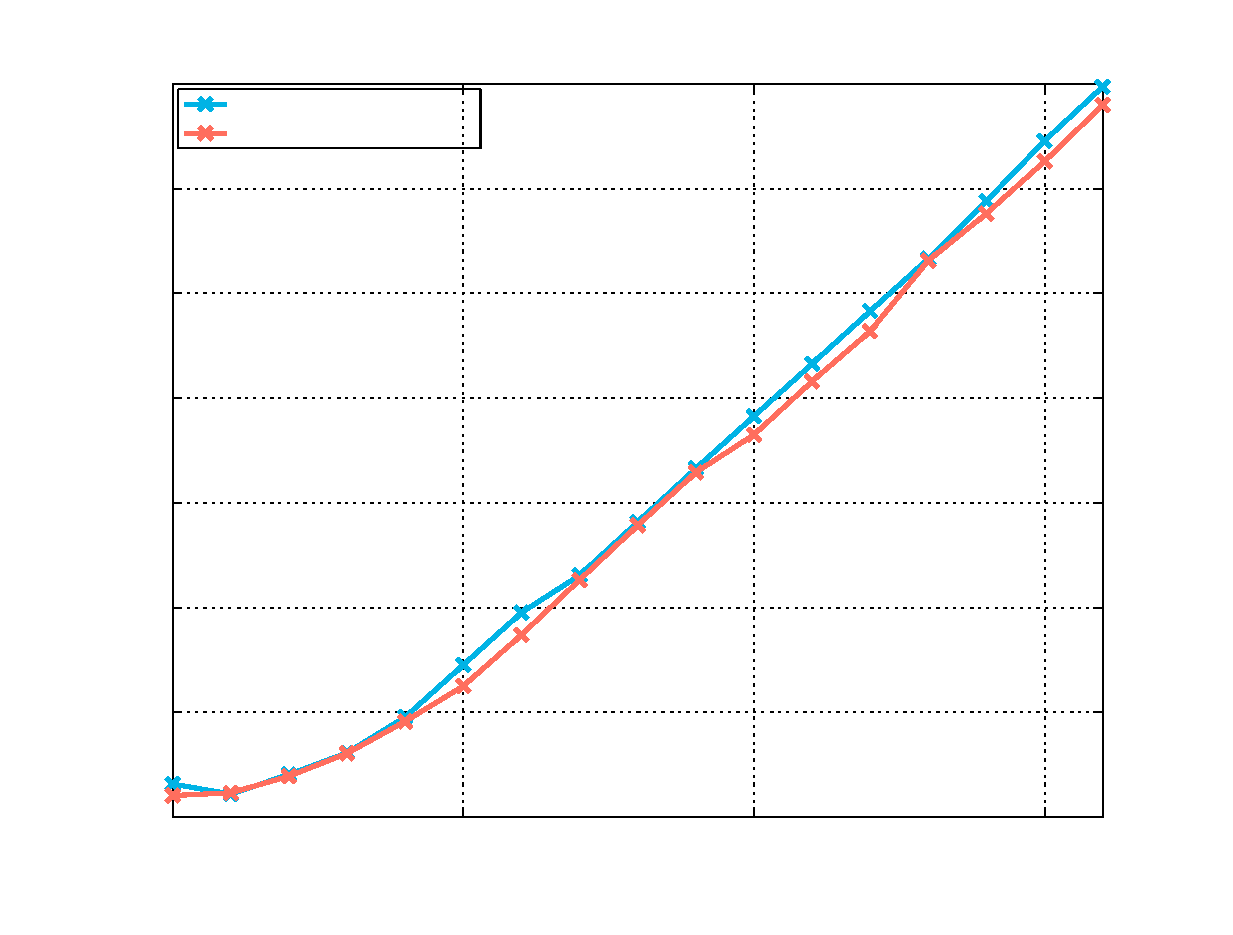
\includegraphics{consexp-inc}
\end{picture}%
\begin{picture}(576,433)(0,0)
\fontsize{10}{0}
\selectfont\put(74.88,43.5189){\makebox(0,0)[t]{\textcolor[rgb]{0,0,0}{{10}}}}
\fontsize{10}{0}
\selectfont\put(214.38,43.5189){\makebox(0,0)[t]{\textcolor[rgb]{0,0,0}{{15}}}}
\fontsize{10}{0}
\selectfont\put(353.88,43.5189){\makebox(0,0)[t]{\textcolor[rgb]{0,0,0}{{20}}}}
\fontsize{10}{0}
\selectfont\put(493.38,43.5189){\makebox(0,0)[t]{\textcolor[rgb]{0,0,0}{{25}}}}
\fontsize{10}{0}
\selectfont\put(69.8755,48.52){\makebox(0,0)[r]{\textcolor[rgb]{0,0,0}{{-10}}}}
\fontsize{10}{0}
\selectfont\put(69.8755,98.8172){\makebox(0,0)[r]{\textcolor[rgb]{0,0,0}{{-8}}}}
\fontsize{10}{0}
\selectfont\put(69.8755,149.114){\makebox(0,0)[r]{\textcolor[rgb]{0,0,0}{{-6}}}}
\fontsize{10}{0}
\selectfont\put(69.8755,199.411){\makebox(0,0)[r]{\textcolor[rgb]{0,0,0}{{-4}}}}
\fontsize{10}{0}
\selectfont\put(69.8755,249.709){\makebox(0,0)[r]{\textcolor[rgb]{0,0,0}{{-2}}}}
\fontsize{10}{0}
\selectfont\put(69.8755,300.006){\makebox(0,0)[r]{\textcolor[rgb]{0,0,0}{{0}}}}
\fontsize{10}{0}
\selectfont\put(69.8755,350.303){\makebox(0,0)[r]{\textcolor[rgb]{0,0,0}{{2}}}}
\fontsize{10}{0}
\selectfont\put(69.8755,400.6){\makebox(0,0)[r]{\textcolor[rgb]{0,0,0}{{4}}}}
\fontsize{10}{0}
\selectfont\put(298.08,32.5189){\makebox(0,0)[t]{\textcolor[rgb]{0,0,0}{{n}}}}
\fontsize{10}{0}
\selectfont\put(49.8755,224.56){\rotatebox{90}{\makebox(0,0)[b]{\textcolor[rgb]{0,0,0}{{logarithm of minimum runtime}}}}}
\fontsize{10}{0}
\selectfont\put(103.667,390.83){\makebox(0,0)[l]{\textcolor[rgb]{0,0,0}{{Dependent Version}}}}
\fontsize{10}{0}
\selectfont\put(103.667,376.775){\makebox(0,0)[l]{\textcolor[rgb]{0,0,0}{{NonDependent Version}}}}
\fontsize{10}{0}
\selectfont\put(298.08,410.6){\makebox(0,0)[b]{\textcolor[rgb]{0,0,0}{{Comparison of runtime for the cons experiment}}}}
\end{picture}
}
\end{figure}

\subsection{split}

This experiment is an extension of the previous one. The difference is that we require tab operation that depends on the length of the sequence. I have chosen for this purpose to identify the middle element.

Also, since we require creating a big-sequence to start with, I have subtracted the results from the previous experiment, so the values are the minimum time to extract the middle element from an increasingly long sequences.

\begin{figure}[H]
\caption{Splitting Experiment}
\scalebox{0.8} {
\begin{picture}(0,0)
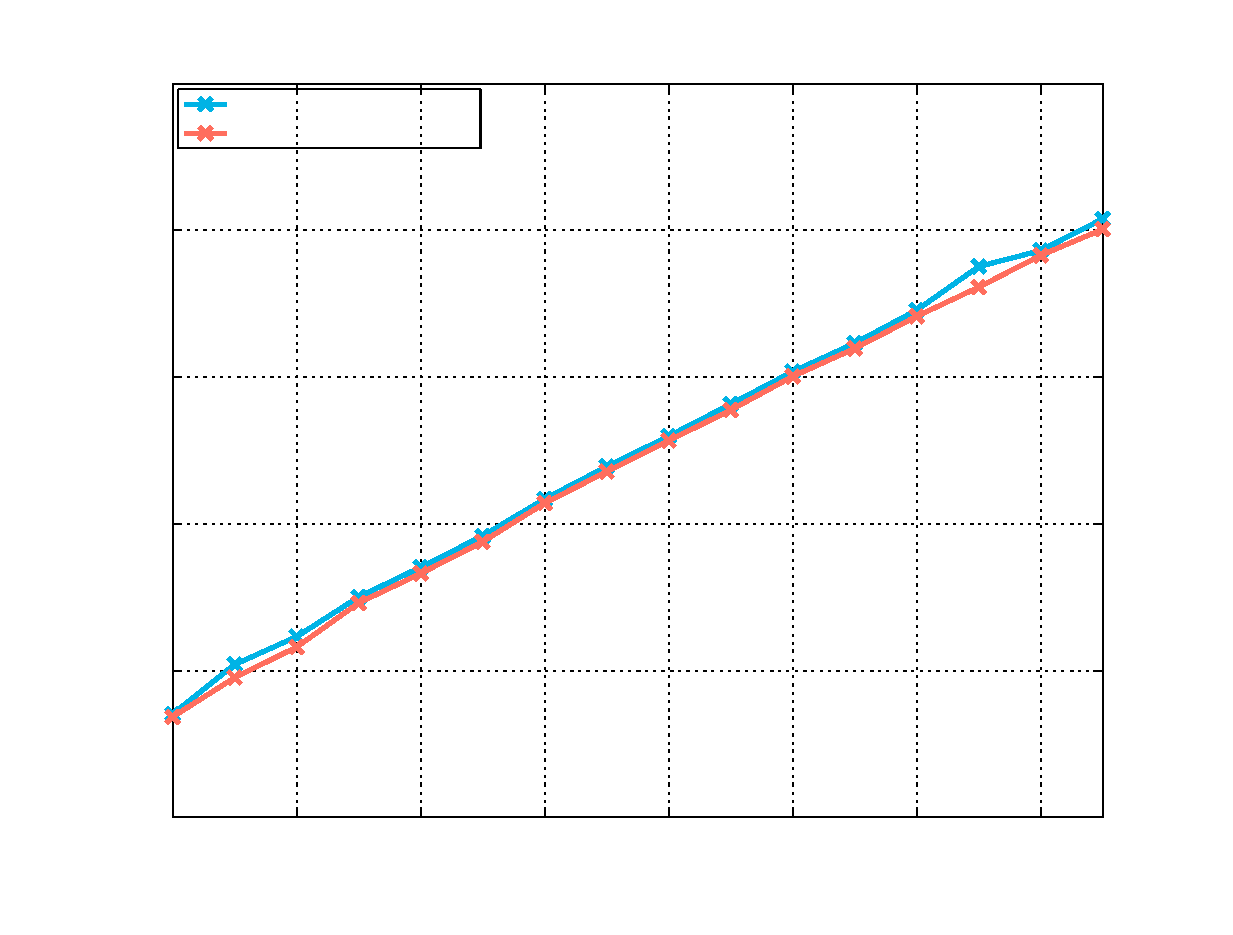
\includegraphics{splitexp-inc}
\end{picture}%
\begin{picture}(576,433)(0,0)
\fontsize{10}{0}
\selectfont\put(72.8,53.3083){\makebox(0,0)[t]{\textcolor[rgb]{0,0,0}{{10}}}}
\fontsize{10}{0}
\selectfont\put(130.667,53.3083){\makebox(0,0)[t]{\textcolor[rgb]{0,0,0}{{12}}}}
\fontsize{10}{0}
\selectfont\put(188.533,53.3083){\makebox(0,0)[t]{\textcolor[rgb]{0,0,0}{{14}}}}
\fontsize{10}{0}
\selectfont\put(246.4,53.3083){\makebox(0,0)[t]{\textcolor[rgb]{0,0,0}{{16}}}}
\fontsize{10}{0}
\selectfont\put(304.267,53.3083){\makebox(0,0)[t]{\textcolor[rgb]{0,0,0}{{18}}}}
\fontsize{10}{0}
\selectfont\put(362.133,53.3083){\makebox(0,0)[t]{\textcolor[rgb]{0,0,0}{{20}}}}
\fontsize{10}{0}
\selectfont\put(420,53.3083){\makebox(0,0)[t]{\textcolor[rgb]{0,0,0}{{22}}}}
\fontsize{10}{0}
\selectfont\put(477.867,53.3083){\makebox(0,0)[t]{\textcolor[rgb]{0,0,0}{{24}}}}
\fontsize{10}{0}
\selectfont\put(67.8,58.31){\makebox(0,0)[r]{\textcolor[rgb]{0,0,0}{{-15}}}}
\fontsize{10}{0}
\selectfont\put(67.8,126.933){\makebox(0,0)[r]{\textcolor[rgb]{0,0,0}{{-10}}}}
\fontsize{10}{0}
\selectfont\put(67.8,195.556){\makebox(0,0)[r]{\textcolor[rgb]{0,0,0}{{-5}}}}
\fontsize{10}{0}
\selectfont\put(67.8,264.179){\makebox(0,0)[r]{\textcolor[rgb]{0,0,0}{{0}}}}
\fontsize{10}{0}
\selectfont\put(67.8,332.802){\makebox(0,0)[r]{\textcolor[rgb]{0,0,0}{{5}}}}
\fontsize{10}{0}
\selectfont\put(67.8,401.425){\makebox(0,0)[r]{\textcolor[rgb]{0,0,0}{{10}}}}
\fontsize{10}{0}
\selectfont\put(289.8,42.3083){\makebox(0,0)[t]{\textcolor[rgb]{0,0,0}{{n}}}}
\fontsize{10}{0}
\selectfont\put(47.8,229.867){\rotatebox{90}{\makebox(0,0)[b]{\textcolor[rgb]{0,0,0}{{logarithm of minimum runtime}}}}}
\fontsize{10}{0}
\selectfont\put(100.787,391.904){\makebox(0,0)[l]{\textcolor[rgb]{0,0,0}{{Dependent Version}}}}
\fontsize{10}{0}
\selectfont\put(100.787,378.206){\makebox(0,0)[l]{\textcolor[rgb]{0,0,0}{{NonDependent Version}}}}
\fontsize{10}{0}
\selectfont\put(289.8,411.425){\makebox(0,0)[b]{\textcolor[rgb]{0,0,0}{{Comparison of runtime for the split experiment}}}}
\end{picture}
}
\end{figure}

I is clear from both these experiments that the dependent versions incurs a higher computational cost. Moreover, the ends show that the divergence between the two depends on the input size.  However, this is not a limitation of dependent types, but of the compiler and extracting tools. All the type annotations could be removed without damaging correctness.

\subsection{reversing and problems with the compiler}

I have tried to repeat the same type of experiment, comparing the run-time of the \textbf{reverse-ft} method, implemented using \textbf{foldl}, and the \textit{rev} method, which uses the \textbf{ViewL}.

Unfortunately, the compilation of the latter method was not successful. Whereas the \textit{normalization} tool always returns the correct result, running a compiled version has caused a \textit{Segmentation Fault} error. This is quite damaging to the application, since a compiler that doesn't preserve the semantics of the code doesn't necessarily preserve correctness. 

\section{Heuristics for Effort}

obviously dependent typed version is harder than a non-dependently typed, see by how much.
probably compare to some other literature?

say that even though it's harder, the system guides you through the proofs.

\subsection{Lines of code}

\begin{itemize}
\item compare version 1 with version 2
\item explain how this is not fully verified, but requires extra proofs --- come back next
\item present sorting as a fully verified procedure and analyze that as a comparison?
\end{itemize}
 
\subsection{Lemma Usage}

\begin{itemize}
\item see how many lemmas are at the base
\item show that some proofs are harder than others?
\item argue the use of the monoid solver
\end{itemize}

\end{document}
